\documentclass[]{book}
\usepackage{lmodern}
\usepackage{amssymb,amsmath}
\usepackage{ifxetex,ifluatex}
\usepackage{fixltx2e} % provides \textsubscript
\ifnum 0\ifxetex 1\fi\ifluatex 1\fi=0 % if pdftex
  \usepackage[T1]{fontenc}
  \usepackage[utf8]{inputenc}
\else % if luatex or xelatex
  \ifxetex
    \usepackage{mathspec}
  \else
    \usepackage{fontspec}
  \fi
  \defaultfontfeatures{Ligatures=TeX,Scale=MatchLowercase}
\fi
% use upquote if available, for straight quotes in verbatim environments
\IfFileExists{upquote.sty}{\usepackage{upquote}}{}
% use microtype if available
\IfFileExists{microtype.sty}{%
\usepackage{microtype}
\UseMicrotypeSet[protrusion]{basicmath} % disable protrusion for tt fonts
}{}
\usepackage{hyperref}
\hypersetup{unicode=true,
            pdftitle={Notas de clase del curso de introducción a Data Science},
            pdfauthor={Diego Kozlowski y Natsumi Shokida},
            pdfborder={0 0 0},
            breaklinks=true}
\urlstyle{same}  % don't use monospace font for urls
\usepackage{natbib}
\bibliographystyle{apalike}
\usepackage{color}
\usepackage{fancyvrb}
\newcommand{\VerbBar}{|}
\newcommand{\VERB}{\Verb[commandchars=\\\{\}]}
\DefineVerbatimEnvironment{Highlighting}{Verbatim}{commandchars=\\\{\}}
% Add ',fontsize=\small' for more characters per line
\usepackage{framed}
\definecolor{shadecolor}{RGB}{248,248,248}
\newenvironment{Shaded}{\begin{snugshade}}{\end{snugshade}}
\newcommand{\AlertTok}[1]{\textcolor[rgb]{0.94,0.16,0.16}{#1}}
\newcommand{\AnnotationTok}[1]{\textcolor[rgb]{0.56,0.35,0.01}{\textbf{\textit{#1}}}}
\newcommand{\AttributeTok}[1]{\textcolor[rgb]{0.77,0.63,0.00}{#1}}
\newcommand{\BaseNTok}[1]{\textcolor[rgb]{0.00,0.00,0.81}{#1}}
\newcommand{\BuiltInTok}[1]{#1}
\newcommand{\CharTok}[1]{\textcolor[rgb]{0.31,0.60,0.02}{#1}}
\newcommand{\CommentTok}[1]{\textcolor[rgb]{0.56,0.35,0.01}{\textit{#1}}}
\newcommand{\CommentVarTok}[1]{\textcolor[rgb]{0.56,0.35,0.01}{\textbf{\textit{#1}}}}
\newcommand{\ConstantTok}[1]{\textcolor[rgb]{0.00,0.00,0.00}{#1}}
\newcommand{\ControlFlowTok}[1]{\textcolor[rgb]{0.13,0.29,0.53}{\textbf{#1}}}
\newcommand{\DataTypeTok}[1]{\textcolor[rgb]{0.13,0.29,0.53}{#1}}
\newcommand{\DecValTok}[1]{\textcolor[rgb]{0.00,0.00,0.81}{#1}}
\newcommand{\DocumentationTok}[1]{\textcolor[rgb]{0.56,0.35,0.01}{\textbf{\textit{#1}}}}
\newcommand{\ErrorTok}[1]{\textcolor[rgb]{0.64,0.00,0.00}{\textbf{#1}}}
\newcommand{\ExtensionTok}[1]{#1}
\newcommand{\FloatTok}[1]{\textcolor[rgb]{0.00,0.00,0.81}{#1}}
\newcommand{\FunctionTok}[1]{\textcolor[rgb]{0.00,0.00,0.00}{#1}}
\newcommand{\ImportTok}[1]{#1}
\newcommand{\InformationTok}[1]{\textcolor[rgb]{0.56,0.35,0.01}{\textbf{\textit{#1}}}}
\newcommand{\KeywordTok}[1]{\textcolor[rgb]{0.13,0.29,0.53}{\textbf{#1}}}
\newcommand{\NormalTok}[1]{#1}
\newcommand{\OperatorTok}[1]{\textcolor[rgb]{0.81,0.36,0.00}{\textbf{#1}}}
\newcommand{\OtherTok}[1]{\textcolor[rgb]{0.56,0.35,0.01}{#1}}
\newcommand{\PreprocessorTok}[1]{\textcolor[rgb]{0.56,0.35,0.01}{\textit{#1}}}
\newcommand{\RegionMarkerTok}[1]{#1}
\newcommand{\SpecialCharTok}[1]{\textcolor[rgb]{0.00,0.00,0.00}{#1}}
\newcommand{\SpecialStringTok}[1]{\textcolor[rgb]{0.31,0.60,0.02}{#1}}
\newcommand{\StringTok}[1]{\textcolor[rgb]{0.31,0.60,0.02}{#1}}
\newcommand{\VariableTok}[1]{\textcolor[rgb]{0.00,0.00,0.00}{#1}}
\newcommand{\VerbatimStringTok}[1]{\textcolor[rgb]{0.31,0.60,0.02}{#1}}
\newcommand{\WarningTok}[1]{\textcolor[rgb]{0.56,0.35,0.01}{\textbf{\textit{#1}}}}
\usepackage{longtable,booktabs}
\usepackage{graphicx,grffile}
\makeatletter
\def\maxwidth{\ifdim\Gin@nat@width>\linewidth\linewidth\else\Gin@nat@width\fi}
\def\maxheight{\ifdim\Gin@nat@height>\textheight\textheight\else\Gin@nat@height\fi}
\makeatother
% Scale images if necessary, so that they will not overflow the page
% margins by default, and it is still possible to overwrite the defaults
% using explicit options in \includegraphics[width, height, ...]{}
\setkeys{Gin}{width=\maxwidth,height=\maxheight,keepaspectratio}
\IfFileExists{parskip.sty}{%
\usepackage{parskip}
}{% else
\setlength{\parindent}{0pt}
\setlength{\parskip}{6pt plus 2pt minus 1pt}
}
\setlength{\emergencystretch}{3em}  % prevent overfull lines
\providecommand{\tightlist}{%
  \setlength{\itemsep}{0pt}\setlength{\parskip}{0pt}}
\setcounter{secnumdepth}{5}
% Redefines (sub)paragraphs to behave more like sections
\ifx\paragraph\undefined\else
\let\oldparagraph\paragraph
\renewcommand{\paragraph}[1]{\oldparagraph{#1}\mbox{}}
\fi
\ifx\subparagraph\undefined\else
\let\oldsubparagraph\subparagraph
\renewcommand{\subparagraph}[1]{\oldsubparagraph{#1}\mbox{}}
\fi

%%% Use protect on footnotes to avoid problems with footnotes in titles
\let\rmarkdownfootnote\footnote%
\def\footnote{\protect\rmarkdownfootnote}

%%% Change title format to be more compact
\usepackage{titling}

% Create subtitle command for use in maketitle
\providecommand{\subtitle}[1]{
  \posttitle{
    \begin{center}\large#1\end{center}
    }
}

\setlength{\droptitle}{-2em}

  \title{Notas de clase del curso de introducción a Data Science}
    \pretitle{\vspace{\droptitle}\centering\huge}
  \posttitle{\par}
    \author{Diego Kozlowski y Natsumi Shokida}
    \preauthor{\centering\large\emph}
  \postauthor{\par}
      \predate{\centering\large\emph}
  \postdate{\par}
    \date{2019-08-23}

\usepackage{booktabs}
\usepackage{amsthm}
\makeatletter
\def\thm@space@setup{%
  \thm@preskip=8pt plus 2pt minus 4pt
  \thm@postskip=\thm@preskip
}
\makeatother

\begin{document}
\maketitle

{
\setcounter{tocdepth}{1}
\tableofcontents
}
\hypertarget{temario}{%
\chapter{Temario}\label{temario}}

\begin{itemize}
\tightlist
\item
  \textbf{clase 1}: Introducción al entorno R
\item
  \textbf{clase 2}: Tidyverse. (limpieza y organización de datos)
\item
  \textbf{clase 3}: Visualización de la información
\item
  \textbf{clase 4}: Estadística descriptiva
\item
  \textbf{clase 5}:
\item
  \textbf{clase 6}:
\item
  \textbf{clase 7}:
\item
  \textbf{clase 8}:
\item
  \textbf{clase 9}:
\item
  \textbf{clase 10}:
\end{itemize}

\hypertarget{librerias-a-instalar}{%
\subsubsection{Librerias a instalar}\label{librerias-a-instalar}}

\begin{verbatim}
install.packages(c("tidyverse","openxlsx",'ggplot2','ggthemes', 'ggrepel','ggalt','kableExtra','GGally','ggridges','fs','purrr','rmarkdown'))
\end{verbatim}

\hypertarget{introduccion-a-r}{%
\chapter{Introducción a R}\label{introduccion-a-r}}

\hypertarget{explicacion}{%
\section{Explicación}\label{explicacion}}

\begin{figure}
\centering

\includegraphics[width=10.41667in,height=\textheight]{img/Rlogo.png}
\caption{\url{https://cran.r-project.org/}}
\end{figure}

\hypertarget{que-es-r}{%
\subsection{¿Que es R?}\label{que-es-r}}

\begin{itemize}
\tightlist
\item
  Lenguaje para el procesamiento y análisis estadístico de datos
\item
  Software Libre
\item
  Sintaxis Básica: R base
\item
  Sintaxis incremental\footnote{Más allá de los comandos elementales, comandos más sofisticados tienen muchas versiones, y algunas quedan en desuso en el tiempo.}: El lenguaje se va ampliando por aportes de Universidades, investigadores/as, usuarios/as y empresas privadas, organizados en librerías (o paquetes)
\item
  Comunidad web muy grande para realizar preguntas y despejar dudas.
\item
  Graficos con calidad de publicación
\end{itemize}

\begin{figure}
\centering
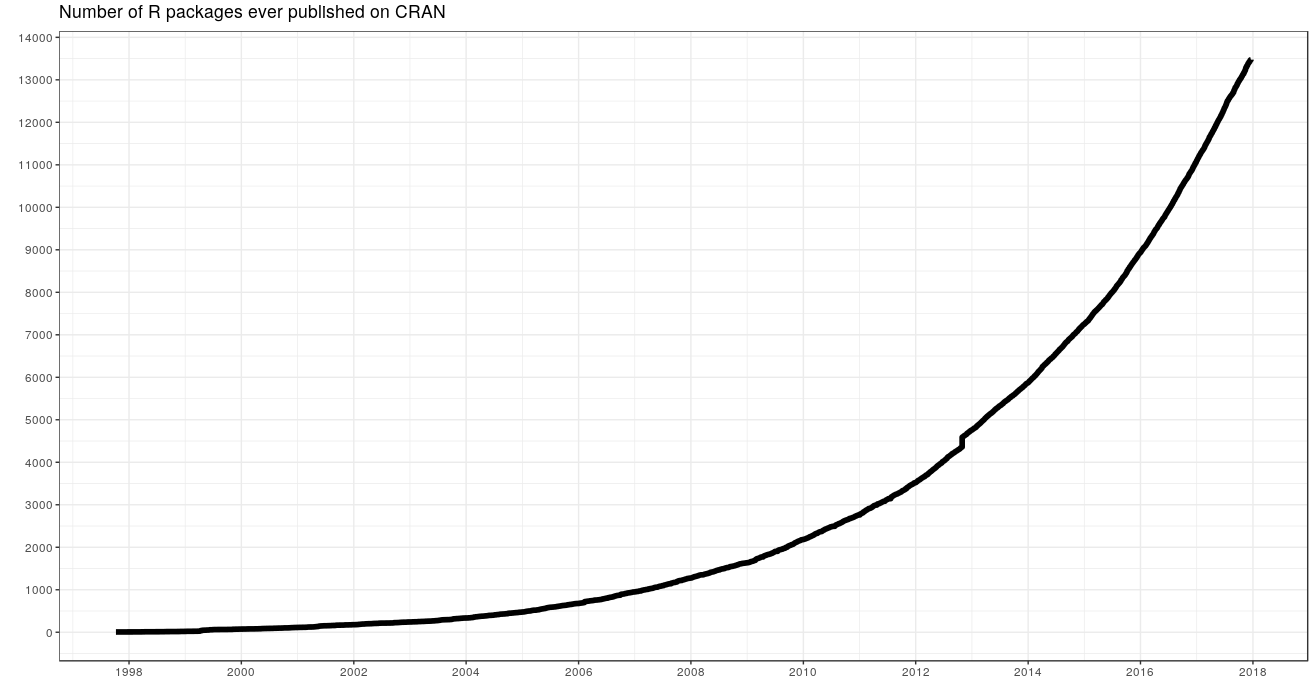
\includegraphics[width=10.41667in,height=\textheight]{img/number-of-submitted-packages-to-CRAN.png}
\caption{fuente: \url{https://gist.github.com/daroczig/3cf06d6db4be2bbe3368}}
\end{figure}

\begin{figure}
\centering

\includegraphics[width=10.41667in,height=\textheight]{img/RStudio-Logo-Flat.png}
\caption{\url{https://www.rstudio.com/}}
\end{figure}

El \emph{entorno} más cómodo para utilizar el \emph{lenguaje} \textbf{R} es el \emph{programa} \textbf{R studio}

\begin{itemize}
\item
  Rstudio es una empresa que produce productos asociados al lenguaje R, como el programa sobre el que corremos los comandos, y extensiones del lenguaje (librerías).
\item
  El programa es \emph{gratuito} y se puede bajar de la
  \href{https://www.rstudio.com/}{página oficial}
\end{itemize}

\begin{figure}
\centering
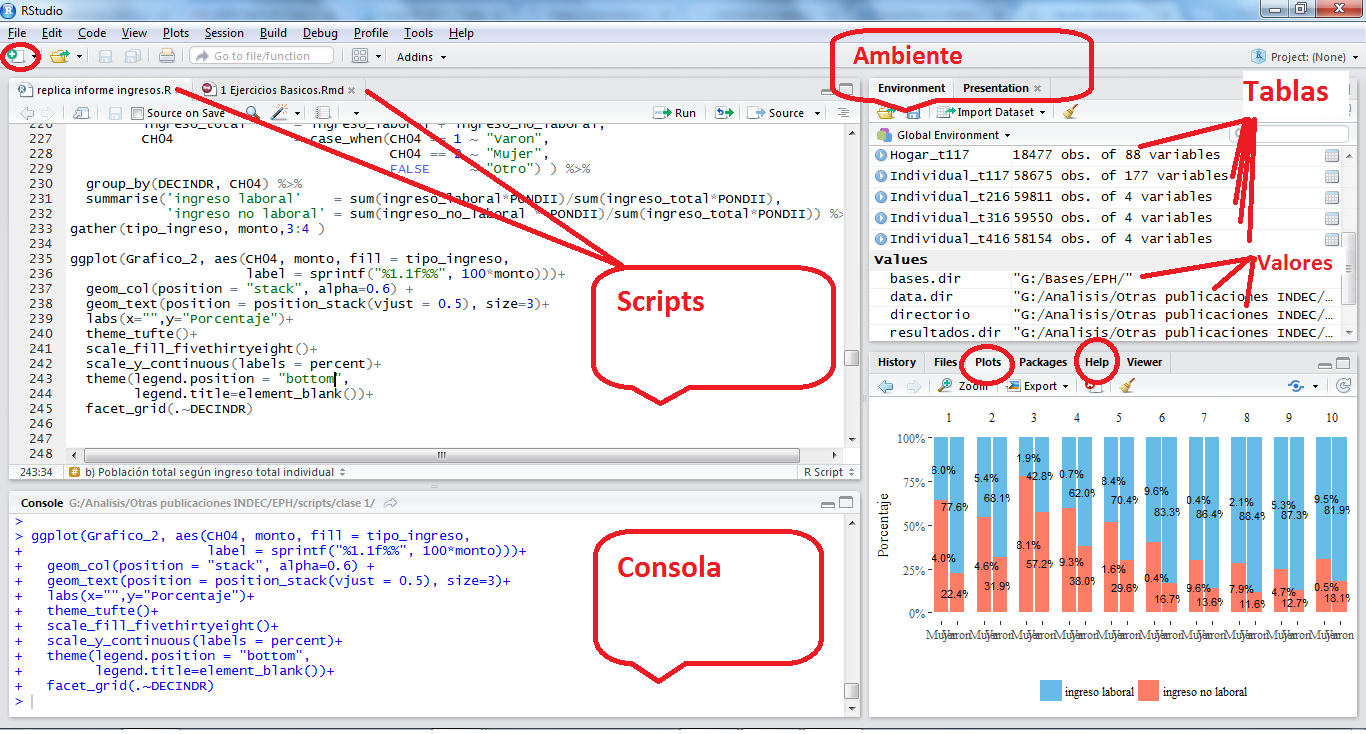
\includegraphics[width=10.41667in,height=\textheight]{img/Pantalla Rstudio.png}
\caption{Pantalla Rstudio}
\end{figure}

\hypertarget{logica-sintactica.}{%
\subsection{Lógica sintáctica.}\label{logica-sintactica.}}

\hypertarget{definicion-de-objetos}{%
\subsubsection{Definición de objetos}\label{definicion-de-objetos}}

Los \textbf{Objetos/Elementos} constituyen la categoría escencial del R. De hecho, todo en R es un objeto, y se almacena con un nombre específico que \textbf{no debe poseer espacios}. Un número, un vector, una función, la progresión de letras del abecedario, una base de datos, un gráfico, constituyen para R objetos de distinto tipo. Los objetos que vamos creando a medida que trabajamos pueden visualizarse en la panel derecho superior de la pantalla.

El operador \textbf{\texttt{\textless{}-}} sirve para definir un objeto. \textbf{A la izquierda} del \textbf{\texttt{\textless{}-}} debe ubicarse el nombre que tomará el elemento a crear. \textbf{Del lado derecho} debe ir la definición del mismo

\begin{Shaded}
\begin{Highlighting}[]
\NormalTok{A <-}\StringTok{ }\DecValTok{1}
\end{Highlighting}
\end{Shaded}

Al definir un elemento, el mismo queda guardado en el ambiente del programa, y podrá ser utilizado posteriormente para observar su contenido o para realizar una operación con el mismo

\begin{Shaded}
\begin{Highlighting}[]
\NormalTok{A }
\end{Highlighting}
\end{Shaded}

\begin{verbatim}
## [1] 1
\end{verbatim}

\begin{Shaded}
\begin{Highlighting}[]
\NormalTok{A}\OperatorTok{+}\DecValTok{6}
\end{Highlighting}
\end{Shaded}

\begin{verbatim}
## [1] 7
\end{verbatim}

Al correr una linea con el nombre del objeto, la consola del programa nos muestra su contenido. Entre Corchetes Observamos el número de orden del elemento en cuestión

El operador \textbf{\texttt{=}} es \textbf{equivalente} a \textbf{\texttt{\textless{}-}}, pero en la práctica no se utiliza para la definición de objetos.

\begin{Shaded}
\begin{Highlighting}[]
\NormalTok{B =}\StringTok{ }\DecValTok{2}
\NormalTok{B}
\end{Highlighting}
\end{Shaded}

\begin{verbatim}
## [1] 2
\end{verbatim}

\textbf{\texttt{\textless{}-}} es un operador \textbf{Unidireccional}, es decir que:\\
\texttt{A\ \textless{}-\ B} implica que \textbf{A} va tomar como valor el contenido del objeto \textbf{B}, y no al revés.

\begin{Shaded}
\begin{Highlighting}[]
\NormalTok{A <-}\StringTok{ }\NormalTok{B}
\NormalTok{A   }\CommentTok{#Ahora A toma el valor de B, y B continua conservando el mismo valor}
\end{Highlighting}
\end{Shaded}

\begin{verbatim}
## [1] 2
\end{verbatim}

\begin{Shaded}
\begin{Highlighting}[]
\NormalTok{B}
\end{Highlighting}
\end{Shaded}

\begin{verbatim}
## [1] 2
\end{verbatim}

\hypertarget{r-base}{%
\subsection{R base}\label{r-base}}

Con \emph{R base} nos referimos a los comandos básicos que vienen incorporados en el R, sin necesidad de cargar librerías.

\hypertarget{operadores-logicos}{%
\subsubsection{Operadores lógicos:}\label{operadores-logicos}}

\begin{itemize}
\tightlist
\item
  \(>\)
\item
  \(>=\)
\item
  \(<\)
\item
  \(<=\)
\item
  \(==\)
\item
  \(!=\)
\end{itemize}

\begin{Shaded}
\begin{Highlighting}[]
\CommentTok{#Redefinimos los valores A y B}
\NormalTok{A <-}\StringTok{  }\DecValTok{10}
\NormalTok{B  <-}\StringTok{  }\DecValTok{20}
\CommentTok{#Realizamos comparaciones lógicas}

\NormalTok{A }\OperatorTok{>}\StringTok{  }\NormalTok{B}
\end{Highlighting}
\end{Shaded}

\begin{verbatim}
## [1] FALSE
\end{verbatim}

\begin{Shaded}
\begin{Highlighting}[]
\NormalTok{A }\OperatorTok{>=}\StringTok{ }\NormalTok{B}
\end{Highlighting}
\end{Shaded}

\begin{verbatim}
## [1] FALSE
\end{verbatim}

\begin{Shaded}
\begin{Highlighting}[]
\NormalTok{A }\OperatorTok{<}\StringTok{  }\NormalTok{B}
\end{Highlighting}
\end{Shaded}

\begin{verbatim}
## [1] TRUE
\end{verbatim}

\begin{Shaded}
\begin{Highlighting}[]
\NormalTok{A }\OperatorTok{<=}\StringTok{ }\NormalTok{B}
\end{Highlighting}
\end{Shaded}

\begin{verbatim}
## [1] TRUE
\end{verbatim}

\begin{Shaded}
\begin{Highlighting}[]
\NormalTok{A }\OperatorTok{==}\StringTok{ }\NormalTok{B}
\end{Highlighting}
\end{Shaded}

\begin{verbatim}
## [1] FALSE
\end{verbatim}

\begin{Shaded}
\begin{Highlighting}[]
\NormalTok{A }\OperatorTok{!=}\StringTok{ }\NormalTok{B}
\end{Highlighting}
\end{Shaded}

\begin{verbatim}
## [1] TRUE
\end{verbatim}

\begin{Shaded}
\begin{Highlighting}[]
\NormalTok{C <-}\StringTok{ }\NormalTok{A }\OperatorTok{!=}\StringTok{ }\NormalTok{B}
\NormalTok{C}
\end{Highlighting}
\end{Shaded}

\begin{verbatim}
## [1] TRUE
\end{verbatim}

Como muestra el último ejemplo, el resultado de una operación lógica puede almacenarse como el valor de un objeto.

\hypertarget{operadores-aritmeticos}{%
\subsubsection{Operadores aritméticos:}\label{operadores-aritmeticos}}

\begin{Shaded}
\begin{Highlighting}[]
\CommentTok{#suma}
\NormalTok{A <-}\StringTok{ }\DecValTok{5}\OperatorTok{+}\DecValTok{6}
\NormalTok{A}
\end{Highlighting}
\end{Shaded}

\begin{verbatim}
## [1] 11
\end{verbatim}

\begin{Shaded}
\begin{Highlighting}[]
\CommentTok{#Resta}
\NormalTok{B <-}\StringTok{ }\DecValTok{6-8}
\NormalTok{B}
\end{Highlighting}
\end{Shaded}

\begin{verbatim}
## [1] -2
\end{verbatim}

\begin{Shaded}
\begin{Highlighting}[]
\CommentTok{#cociente}
\NormalTok{C <-}\StringTok{ }\DecValTok{6}\OperatorTok{/}\FloatTok{2.5}
\NormalTok{C}
\end{Highlighting}
\end{Shaded}

\begin{verbatim}
## [1] 2.4
\end{verbatim}

\begin{Shaded}
\begin{Highlighting}[]
\CommentTok{#multiplicacion}
\NormalTok{D <-}\StringTok{ }\DecValTok{6}\OperatorTok{*}\FloatTok{2.5}
\NormalTok{D}
\end{Highlighting}
\end{Shaded}

\begin{verbatim}
## [1] 15
\end{verbatim}

\hypertarget{funciones}{%
\subsubsection{Funciones:}\label{funciones}}

Las funciones son series de procedimientos estandarizados, que toman como imput determinados argumentos a fijar por el usuario, y devuelven un resultado acorde a la aplicación de dichos procedimientos. Su lógica de funcionamiento es:\\
\texttt{funcion(argumento1\ =\ arg1,\ argumento2\ =\ arg2)}

A lo largo del curso iremos viendo numerosas funciones, según lo requieran los distintos ejercicios. Sin embargo, veamos ahora algunos ejemplos para comprender su funcionamiento:

\begin{itemize}
\tightlist
\item
  paste() : concatena una serie de caracteres, indicando por última instancia como separar a cada uno de ellos\\
\item
  paste0(): concatena una serie de caracteres sin separar
\item
  sum(): suma de todos los elementos de un vector\\
\item
  mean() promedio aritmético de todos los elementos de un vector
\end{itemize}

\begin{Shaded}
\begin{Highlighting}[]
\KeywordTok{paste}\NormalTok{(}\StringTok{"Pega"}\NormalTok{,}\StringTok{"estas"}\NormalTok{,}\DecValTok{4}\NormalTok{,}\StringTok{"palabras"}\NormalTok{, }\DataTypeTok{sep =} \StringTok{" "}\NormalTok{)}
\end{Highlighting}
\end{Shaded}

\begin{verbatim}
## [1] "Pega estas 4 palabras"
\end{verbatim}

\begin{Shaded}
\begin{Highlighting}[]
\CommentTok{#Puedo concatenar caracteres almacenados en objetos}
\KeywordTok{paste}\NormalTok{(A,B,C,}\DataTypeTok{sep =} \StringTok{"**"}\NormalTok{)}
\end{Highlighting}
\end{Shaded}

\begin{verbatim}
## [1] "11**-2**2.4"
\end{verbatim}

\begin{Shaded}
\begin{Highlighting}[]
\CommentTok{# Paste0 pega los caracteres sin separador}
\KeywordTok{paste0}\NormalTok{(A,B,C)}
\end{Highlighting}
\end{Shaded}

\begin{verbatim}
## [1] "11-22.4"
\end{verbatim}

\begin{Shaded}
\begin{Highlighting}[]
\DecValTok{1}\OperatorTok{:}\DecValTok{5}
\end{Highlighting}
\end{Shaded}

\begin{verbatim}
## [1] 1 2 3 4 5
\end{verbatim}

\begin{Shaded}
\begin{Highlighting}[]
\KeywordTok{sum}\NormalTok{(}\DecValTok{1}\OperatorTok{:}\DecValTok{5}\NormalTok{)}
\end{Highlighting}
\end{Shaded}

\begin{verbatim}
## [1] 15
\end{verbatim}

\begin{Shaded}
\begin{Highlighting}[]
\KeywordTok{mean}\NormalTok{(}\DecValTok{1}\OperatorTok{:}\DecValTok{5}\NormalTok{,}\DataTypeTok{na.rm =} \OtherTok{TRUE}\NormalTok{)}
\end{Highlighting}
\end{Shaded}

\begin{verbatim}
## [1] 3
\end{verbatim}

\hypertarget{caracteres-especiales}{%
\subsubsection{Caracteres especiales}\label{caracteres-especiales}}

\begin{itemize}
\tightlist
\item
  R es sensible a mayúsculas y minúsculas, tanto para los nombres de las variables, como para las funciones y parámetros.
\item
  Los \textbf{espacios en blanco} y los \textbf{carriage return} (\emph{enter}) no son considerados por el lenguaje. Los podemos aprovechar para emprolijar el código y que la lectura sea más simple\footnote{veremos que existen ciertas excepciones con algunos paquetes más adelante.}.
\end{itemize}

\begin{itemize}
\item
  El \textbf{numeral} \texttt{\#} se utiliza para hacer comentarios. Todo lo que se escribe después del \# no es interpretado por R. Se debe utilizar un \# por cada línea de código que se desea anular
\item
  Los \textbf{corchetes} \texttt{{[}{]}} se utilizan para acceder a un objeto:

  \begin{itemize}
  \tightlist
  \item
    en un vector{[}n° orden{]}
  \item
    en una tabla{[}fila, columna{]}
  \item
    en una lista{[}n° elemento{]}
  \end{itemize}
\item
  el signo \textbf{\$} también es un método de acceso. Particularmente, en los dataframes, nos permitira acceder a una determinada columna de una tabla
\item
  Los \textbf{paréntesis}\texttt{()} se utilizan en las funciones para definir los parámetros.
\item
  Las \textbf{comas} \texttt{,} se utilizan para separar los parametros al interior de una función.
\end{itemize}

\hypertarget{objetos}{%
\subsection{Objetos:}\label{objetos}}

Existen un gran cantidad de objetos distintos en R, en lo que resepcta al curso trabajaremos principalmente con 3 de ellos:

\begin{itemize}
\tightlist
\item
  Valores
\item
  Vectores
\item
  Data Frames
\item
  Listas
\end{itemize}

\hypertarget{valores}{%
\subsubsection{Valores}\label{valores}}

Los valores y vectores pueden ser a su vez de distintas \emph{clases}:

\textbf{Numeric}

\begin{Shaded}
\begin{Highlighting}[]
\NormalTok{A <-}\StringTok{  }\DecValTok{1}
\KeywordTok{class}\NormalTok{(A)}
\end{Highlighting}
\end{Shaded}

\begin{verbatim}
## [1] "numeric"
\end{verbatim}

\textbf{Character}

\begin{Shaded}
\begin{Highlighting}[]
\NormalTok{A <-}\StringTok{  }\KeywordTok{paste}\NormalTok{(}\StringTok{'Soy'}\NormalTok{, }\StringTok{'una'}\NormalTok{, }\StringTok{'concatenación', '}\NormalTok{de}\StringTok{', '}\NormalTok{caracteres}\StringTok{', sep = " ")}
\StringTok{A}
\end{Highlighting}
\end{Shaded}

\begin{verbatim}
## [1] "Soy una concatenación de caracteres"
\end{verbatim}

\begin{Shaded}
\begin{Highlighting}[]
\KeywordTok{class}\NormalTok{(A)}
\end{Highlighting}
\end{Shaded}

\begin{verbatim}
## [1] "character"
\end{verbatim}

\textbf{Factor}

\begin{Shaded}
\begin{Highlighting}[]
\NormalTok{A <-}\StringTok{ }\KeywordTok{factor}\NormalTok{(}\StringTok{"Soy un factor, con niveles fijos"}\NormalTok{)}
\KeywordTok{class}\NormalTok{(A)}
\end{Highlighting}
\end{Shaded}

\begin{verbatim}
## [1] "factor"
\end{verbatim}

La diferencia entre un \emph{character} y un \emph{factor} es que el último tiene solo algunos valores permitidos (levels), con un orden interno predefinido (el cual ,por ejemplo, se respetará a la hora de realizar un gráfico)

\hypertarget{vectores}{%
\subsubsection{Vectores}\label{vectores}}

Para crear un \textbf{vector} utilizamos el comando \texttt{c()}, de combinar.

\begin{Shaded}
\begin{Highlighting}[]
\NormalTok{C <-}\StringTok{ }\KeywordTok{c}\NormalTok{(}\DecValTok{1}\NormalTok{, }\DecValTok{3}\NormalTok{, }\DecValTok{4}\NormalTok{)}
\NormalTok{C}
\end{Highlighting}
\end{Shaded}

\begin{verbatim}
## [1] 1 3 4
\end{verbatim}

sumarle 2 a cada elemento del \textbf{vector} anterior

\begin{Shaded}
\begin{Highlighting}[]
\NormalTok{C <-}\StringTok{ }\NormalTok{C }\OperatorTok{+}\StringTok{ }\DecValTok{2}
\NormalTok{C}
\end{Highlighting}
\end{Shaded}

\begin{verbatim}
## [1] 3 5 6
\end{verbatim}

sumarle 1 al primer elemento, 2 al segundo, y 3 al tercer elemento del \textbf{vector} anterior

\begin{Shaded}
\begin{Highlighting}[]
\NormalTok{D <-}\StringTok{ }\NormalTok{C }\OperatorTok{+}\StringTok{ }\DecValTok{1}\OperatorTok{:}\DecValTok{3} \CommentTok{#esto es equivalente a hacer 3+1, 5+2, 6+9 }
\NormalTok{D}
\end{Highlighting}
\end{Shaded}

\begin{verbatim}
## [1] 4 7 9
\end{verbatim}

\texttt{1:3} significa que queremos todos los números enteros desde 1 hasta 3.

crear un \textbf{vector} que contenga las palabras: ``Carlos'',``Federico'',``Pedro''

\begin{Shaded}
\begin{Highlighting}[]
\NormalTok{E <-}\StringTok{ }\KeywordTok{c}\NormalTok{(}\StringTok{"Carlos"}\NormalTok{,}\StringTok{"Federico"}\NormalTok{,}\StringTok{"Pedro"}\NormalTok{)}
\NormalTok{E}
\end{Highlighting}
\end{Shaded}

\begin{verbatim}
## [1] "Carlos"   "Federico" "Pedro"
\end{verbatim}

para acceder a algún elemento del vector, podemos buscarlo por su número de orden, entre \texttt{{[}\ {]}}

\begin{Shaded}
\begin{Highlighting}[]
\NormalTok{ E[}\DecValTok{2}\NormalTok{]}
\end{Highlighting}
\end{Shaded}

\begin{verbatim}
## [1] "Federico"
\end{verbatim}

Si nos interesa almacenar dicho valor, al buscarlo lo asignamos a un nuevo objeto, dandole el nombre que deseemos

\begin{Shaded}
\begin{Highlighting}[]
\NormalTok{elemento2 <-}\StringTok{  }\NormalTok{E[}\DecValTok{2}\NormalTok{]}
\end{Highlighting}
\end{Shaded}

\begin{Shaded}
\begin{Highlighting}[]
\NormalTok{elemento2}
\end{Highlighting}
\end{Shaded}

\begin{verbatim}
## [1] "Federico"
\end{verbatim}

para \textbf{borrar} un objeto del ambiente de trabajo, utilizamos el comando \emph{\texttt{rm()}}

\begin{Shaded}
\begin{Highlighting}[]
\KeywordTok{rm}\NormalTok{(elemento2)}
\NormalTok{elemento2}
\end{Highlighting}
\end{Shaded}

\begin{verbatim}
## Error in eval(expr, envir, enclos): object 'elemento2' not found
\end{verbatim}

También podemos cambiar el texto del segundo elemento de E, por el texto ``Pablo''

\begin{Shaded}
\begin{Highlighting}[]
\NormalTok{E[}\DecValTok{2}\NormalTok{] <-}\StringTok{ "Pablo"}
\NormalTok{E}
\end{Highlighting}
\end{Shaded}

\begin{verbatim}
## [1] "Carlos" "Pablo"  "Pedro"
\end{verbatim}

\hypertarget{data-frames}{%
\subsection{Data Frames}\label{data-frames}}

Un Data Frame es una tabla de datos, donde cada columna representa una variable, y cada fila una observación.

Este objeto suele ser central en el proceso de trabajo, y suele ser la forma en que se cargan datos externos para trabajar en el ambiente de R, y en que se exportan los resultados de nuestros trabajo.

También Se puede crear como la combinación de N vectores de igual tamaño. Por ejemplo, tomamos algunos valores del \href{http://www.indec.gob.ar/bajarCuadroEstadistico.asp?idc=4020B33440609462654542BD0BC320F1523DA0DC52C396201DB4DD5861FFEDC9AD1436681AC84179}{Indice de salarios}

\begin{Shaded}
\begin{Highlighting}[]
\NormalTok{INDICE  <-}\StringTok{ }\KeywordTok{c}\NormalTok{(}\DecValTok{100}\NormalTok{,   }\DecValTok{100}\NormalTok{,   }\DecValTok{100}\NormalTok{,}
             \FloatTok{101.8}\NormalTok{, }\FloatTok{101.2}\NormalTok{, }\FloatTok{100.73}\NormalTok{,}
             \FloatTok{102.9}\NormalTok{, }\FloatTok{102.4}\NormalTok{, }\FloatTok{103.2}\NormalTok{)}

\NormalTok{FECHA  <-}\StringTok{  }\KeywordTok{c}\NormalTok{(}\StringTok{"Oct-16"}\NormalTok{, }\StringTok{"Oct-16"}\NormalTok{, }\StringTok{"Oct-16"}\NormalTok{,}
             \StringTok{"Nov-16"}\NormalTok{, }\StringTok{"Nov-16"}\NormalTok{, }\StringTok{"Nov-16"}\NormalTok{,}
             \StringTok{"Dic-16"}\NormalTok{, }\StringTok{"Dic-16"}\NormalTok{, }\StringTok{"Dic-16"}\NormalTok{)}


\NormalTok{GRUPO  <-}\StringTok{  }\KeywordTok{c}\NormalTok{(}\StringTok{"Privado_Registrado"}\NormalTok{,}\StringTok{"Público","}\NormalTok{Privado_No_Registrado}\StringTok{",}
\StringTok{             "}\NormalTok{Privado_Registrado}\StringTok{","}\NormalTok{Público",}\StringTok{"Privado_No_Registrado"}\NormalTok{,}
             \StringTok{"Privado_Registrado"}\NormalTok{,}\StringTok{"Público","}\NormalTok{Privado_No_Registrado}\StringTok{")}
\StringTok{             }

\StringTok{Datos <- data.frame(INDICE, FECHA, GRUPO)}
\StringTok{Datos}
\end{Highlighting}
\end{Shaded}

\begin{verbatim}
##   INDICE  FECHA                 GRUPO
## 1 100.00 Oct-16    Privado_Registrado
## 2 100.00 Oct-16               Público
## 3 100.00 Oct-16 Privado_No_Registrado
## 4 101.80 Nov-16    Privado_Registrado
## 5 101.20 Nov-16               Público
## 6 100.73 Nov-16 Privado_No_Registrado
## 7 102.90 Dic-16    Privado_Registrado
## 8 102.40 Dic-16               Público
## 9 103.20 Dic-16 Privado_No_Registrado
\end{verbatim}

Tal como en un \textbf{vector} se ubica a los elementos mediante \texttt{{[}\ {]}}, en un \textbf{dataframe} se obtienen sus elementos de la forma \textbf{\texttt{{[}fila,\ columna{]}}}.

Otra opción es especificar la columna, mediante el operador \textbf{\texttt{\$}}, y luego seleccionar dentro de esa columna el registro deseado mediante el número de orden.

\begin{Shaded}
\begin{Highlighting}[]
\NormalTok{Datos}\OperatorTok{$}\NormalTok{FECHA}
\end{Highlighting}
\end{Shaded}

\begin{verbatim}
## [1] Oct-16 Oct-16 Oct-16 Nov-16 Nov-16 Nov-16 Dic-16 Dic-16 Dic-16
## Levels: Dic-16 Nov-16 Oct-16
\end{verbatim}

\begin{Shaded}
\begin{Highlighting}[]
\NormalTok{Datos[}\DecValTok{3}\NormalTok{,}\DecValTok{2}\NormalTok{]}
\end{Highlighting}
\end{Shaded}

\begin{verbatim}
## [1] Oct-16
## Levels: Dic-16 Nov-16 Oct-16
\end{verbatim}

\begin{Shaded}
\begin{Highlighting}[]
\NormalTok{Datos}\OperatorTok{$}\NormalTok{FECHA[}\DecValTok{3}\NormalTok{]}
\end{Highlighting}
\end{Shaded}

\begin{verbatim}
## [1] Oct-16
## Levels: Dic-16 Nov-16 Oct-16
\end{verbatim}

¿que pasa si hacemos \texttt{Datos\$FECHA{[}3,2{]}} ?

\begin{Shaded}
\begin{Highlighting}[]
\NormalTok{Datos}\OperatorTok{$}\NormalTok{FECHA[}\DecValTok{3}\NormalTok{,}\DecValTok{2}\NormalTok{]}
\end{Highlighting}
\end{Shaded}

\begin{verbatim}
## Error in `[.default`(Datos$FECHA, 3, 2): incorrect number of dimensions
\end{verbatim}

Nótese que el último comando tiene un número incorrecto de dimensiones, porque estamos refiriendonos 2 veces a la columna FECHA.

Acorde a lo visto anteriormente, el acceso a los \textbf{dataframes} mediante \texttt{{[}\ {]}}, puede utilizarse para realizar filtros sobre la base, especificando una condición para las filas. Por ejemplo, puedo utilizar los \texttt{{[}\ {]}} para conservar del \textbf{dataframe} \texttt{Datos} unicamente los registros con fecha de Diciembre 2016:

\begin{Shaded}
\begin{Highlighting}[]
\NormalTok{Datos[Datos}\OperatorTok{$}\NormalTok{FECHA}\OperatorTok{==}\StringTok{"Dic-16"}\NormalTok{,]}
\end{Highlighting}
\end{Shaded}

\begin{verbatim}
##   INDICE  FECHA                 GRUPO
## 7  102.9 Dic-16    Privado_Registrado
## 8  102.4 Dic-16               Público
## 9  103.2 Dic-16 Privado_No_Registrado
\end{verbatim}

La lógica del paso anterior sería: Accedo al dataframe \texttt{Datos}, pidiendo únicamente conservar las filas (por eso la condición se ubica a la \emph{izquierda} de la \texttt{,}) que cumplan el requisito de pertenecer a la categoría \textbf{``Dic-16''} de la variable \textbf{FECHA}.\\
Aún más, podría aplicar el filtro y al mismo tiempo identificar una variable de interés para luego realizar un cálculo sobre aquella. Por ejemplo, podría calcular la media de los indices en el mes de Diciembre.

\begin{Shaded}
\begin{Highlighting}[]
\CommentTok{###Por separado}
\NormalTok{Indices_Dic <-}\StringTok{ }\NormalTok{Datos}\OperatorTok{$}\NormalTok{INDICE[Datos}\OperatorTok{$}\NormalTok{FECHA}\OperatorTok{==}\StringTok{"Dic-16"}\NormalTok{]}
\NormalTok{Indices_Dic}
\end{Highlighting}
\end{Shaded}

\begin{verbatim}
## [1] 102.9 102.4 103.2
\end{verbatim}

\begin{Shaded}
\begin{Highlighting}[]
\KeywordTok{mean}\NormalTok{(Indices_Dic)}
\end{Highlighting}
\end{Shaded}

\begin{verbatim}
## [1] 102.8333
\end{verbatim}

\begin{Shaded}
\begin{Highlighting}[]
\CommentTok{### Todo junto}
\KeywordTok{mean}\NormalTok{(Datos}\OperatorTok{$}\NormalTok{INDICE[Datos}\OperatorTok{$}\NormalTok{FECHA}\OperatorTok{==}\StringTok{"Dic-16"}\NormalTok{])}
\end{Highlighting}
\end{Shaded}

\begin{verbatim}
## [1] 102.8333
\end{verbatim}

La lógica de esta sintaxis sería: ``Me quedó con la variable \textbf{INDICE}, cuando la variable FECHA sea igual a \textbf{"Dic-16"}, luego calculo la media de dichos valores''

\hypertarget{listas}{%
\subsection{Listas}\label{listas}}

Contienen una concatenación de objetos de cualquier tipo. Así como un vector contiene valores, un dataframe contiene vectores, una lista puede contener dataframes, pero también vectores, o valores, y \emph{todo ello a la vez}

\begin{Shaded}
\begin{Highlighting}[]
\NormalTok{superlista <-}\StringTok{ }\KeywordTok{list}\NormalTok{(A,B,C,D,E,FECHA, }\DataTypeTok{DF =}\NormalTok{ Datos, INDICE, GRUPO)}
\NormalTok{superlista}
\end{Highlighting}
\end{Shaded}

\begin{verbatim}
## [[1]]
## [1] Soy un factor, con niveles fijos
## Levels: Soy un factor, con niveles fijos
## 
## [[2]]
## [1] -2
## 
## [[3]]
## [1] 3 5 6
## 
## [[4]]
## [1] 4 7 9
## 
## [[5]]
## [1] "Carlos" "Pablo"  "Pedro" 
## 
## [[6]]
## [1] "Oct-16" "Oct-16" "Oct-16" "Nov-16" "Nov-16" "Nov-16" "Dic-16" "Dic-16"
## [9] "Dic-16"
## 
## $DF
##   INDICE  FECHA                 GRUPO
## 1 100.00 Oct-16    Privado_Registrado
## 2 100.00 Oct-16               Público
## 3 100.00 Oct-16 Privado_No_Registrado
## 4 101.80 Nov-16    Privado_Registrado
## 5 101.20 Nov-16               Público
## 6 100.73 Nov-16 Privado_No_Registrado
## 7 102.90 Dic-16    Privado_Registrado
## 8 102.40 Dic-16               Público
## 9 103.20 Dic-16 Privado_No_Registrado
## 
## [[8]]
## [1] 100.00 100.00 100.00 101.80 101.20 100.73 102.90 102.40 103.20
## 
## [[9]]
## [1] "Privado_Registrado"    "Público"               "Privado_No_Registrado"
## [4] "Privado_Registrado"    "Público"               "Privado_No_Registrado"
## [7] "Privado_Registrado"    "Público"               "Privado_No_Registrado"
\end{verbatim}

Para acceder un elemento de una lista, podemos utilizar el operador \textbf{\texttt{\$}}, que se puede usar a su vez de forma iterativa

\begin{Shaded}
\begin{Highlighting}[]
\NormalTok{superlista}\OperatorTok{$}\NormalTok{DF}\OperatorTok{$}\NormalTok{FECHA[}\DecValTok{2}\NormalTok{]}
\end{Highlighting}
\end{Shaded}

\begin{verbatim}
## [1] Oct-16
## Levels: Dic-16 Nov-16 Oct-16
\end{verbatim}

\hypertarget{ambientes-de-trabajo}{%
\subsection{Ambientes de trabajo}\label{ambientes-de-trabajo}}

Hay algunas cosas que tenemos que tener en cuenta respecto del orden del ambiente en el que trabajamos:

\begin{itemize}
\tightlist
\item
  Working Directory: El directorio de trabajo, pueden ver el suyo con \texttt{getwd()}, es \emph{hacia donde apunta el código}, por ejemplo, si quieren leer un archivo, la ruta del archivo tiene que estar explicitada como el recorrido desde el Working Directory.
\item
  Environment: Esto engloba tanto la información que tenemos cargada en \emph{Data} y \emph{Values}, como las librerías que tenemos cargadas mientras trabajamos.
\end{itemize}

Es importante que mantengamos bien delimitadas estas cosas entre diferentes trabajos, sino:

\begin{enumerate}
\def\labelenumi{\arabic{enumi}.}
\tightlist
\item
  El directorio queda referido a un lugar específico en nuestra computadora.
\end{enumerate}

\begin{itemize}
\tightlist
\item
  Si se lo compartimos a otro \textbf{se rompe}
\item
  Si cambiamos de computadora \textbf{se rompe}
\item
  Si lo cambiamos de lugar \textbf{se rompe}
\item
  Si primero abrimos otro script \textbf{se rompe}
\end{itemize}

\begin{enumerate}
\def\labelenumi{\arabic{enumi}.}
\setcounter{enumi}{1}
\tightlist
\item
  Tenemos mezclados resultados de diferentes trabajos:
\end{enumerate}

\begin{itemize}
\tightlist
\item
  Nunca sabemos si esa variable/tabla/lista se creo en ese script y no otro
\item
  Perdemos espacio de la memoria
\item
  No estamos seguros de que el script cargue todas las librerías que necesita
\end{itemize}

Rstudio tiene una herramienta muy útil de trabajo que son los \textbf{proyectos}. Estos permiten mantener un ambiente de trabajo delimitado por cada uno de nuestros trabajos. Es decir:

\begin{itemize}
\tightlist
\item
  El directorio de trabajo se refiere a donde esta ubicado el archivo .Rproj
\item
  El Environment es específico de nuestro proyecto.
\end{itemize}

Un proyecto no es un sólo script, sino toda una carpeta de trabajo.

\begin{figure}
\centering

\includegraphics[width=10.41667in,height=\textheight]{img/Rproject.png}
\caption{logo Rpoject}
\end{figure}

Para crearlo, vamos al logo de nuevo projecto (Arriba a la izquierda de la panatalla), y elegimos la carpeta de trabajo.

\hypertarget{tipos-de-archivos-de-r}{%
\subsection{Tipos de archivos de R}\label{tipos-de-archivos-de-r}}

\begin{itemize}
\tightlist
\item
  \textbf{Script}: Es un archivo de texto plano, donde podemos poner el código que utilizamos para preservarlo
\item
  \textbf{Rnotebook}: También sirve para guardar el código, pero a diferencia de los scripts, se puede compilar, e intercalar código con resultados (este archivo es un rnotebook)
\item
  \textbf{Rproject}: Es un archivo que define la metadata del proyecto
\item
  \textbf{RDS y Rdata}: Dos formatos de archivos propios de R para guardar datos.
\end{itemize}

\hypertarget{practica-guiada}{%
\section{Práctica Guiada}\label{practica-guiada}}

\hypertarget{instalacion-de-paquetes-complementarios-al-r-base}{%
\subsection{Instalación de paquetes complementarios al R Base}\label{instalacion-de-paquetes-complementarios-al-r-base}}

Hasta aquí hemos visto múltiples funciones que están contenidas dentro del lenguaje básico de R. Ahora bien, al tratarse de un software libre, los usuarios de R con más experiencia contribuyen sistemáticamente a expandir este lenguaje mediante la creación y actualización de \textbf{paquetes} complementarios. Lógicamente, los mismos no están incluidos en la instalación inicial del programa, pero podemos descargarlos e instalarlos al mismo tiempo con el siguiente comando:

\begin{verbatim}
install.packages("nombre_del_paquete") 
\end{verbatim}

Resulta recomendable \textbf{ejecutar este comando desde la consola} ya que solo necesitaremos correrlo una vez en nuestra computadora. Al ejecutar el mismo, se descargarán de la pagina de \href{www.cran.r-project.org}{CRAN} los archivos correspondientes al paquete hacia el directorio en donde hayamos instalado el programa. Típicamente los archivos se encontrarán en \textbf{\texttt{C:\textbackslash{}Program\ Files\textbackslash{}R\textbackslash{}R-3.5.0\textbackslash{}library\textbackslash{}}}, siempre con la versión del programa correspondiente.\\
Una vez instalado el paquete, cada vez que abramos una nueva sesión de R y querramos utilizar el mismo debemos \textbf{cargarlo al ambiente de trabajo} mediante la siguiente función:

\begin{verbatim}
library(nombre_del_paquete)
\end{verbatim}

Nótese que al cargar/activar el paquete no son necesarias las comillas.

\hypertarget{lectura-y-escritura-de-archivos}{%
\subsection{Lectura y escritura de archivos}\label{lectura-y-escritura-de-archivos}}

\hypertarget{csv-y-.txt}{%
\subsubsection{.csv y .txt}\label{csv-y-.txt}}

Hay \textbf{muchas} funciones para leer archivos de tipo \emph{.txt} y \emph{.csv}. La mayoría sólo cambia los parámetros que vienen por default.

Es importante tener en cuenta que una base de datos que proviene de archivos \emph{.txt}, o \emph{.csv} puede presentar diferencias en cuanto a los siguientes parametros:

\begin{itemize}
\tightlist
\item
  encabezado
\item
  delimitador (\texttt{,}, tab, \texttt{;})
\item
  separador decimal
\end{itemize}

\begin{verbatim}
dataframe <- read.delim(file, header = TRUE, sep = "\t", quote = "\"", dec = ".", fill = TRUE, comment.char = "", ...) 
\end{verbatim}

Ejemplo. Levantar la base de \href{https://data.buenosaires.gob.ar/dataset/sueldo-funcionarios}{sueldos de funcionarios}

En el parametro \texttt{file} tengo que especificar el nombre completo del archivo, incluyendo el directorio donde se encuentra. Lo más sencillo es abrir comillas, apretar \texttt{Tab} y se despliega el menú de las cosas que tenemos en el directorio de trabajo. Si queremos movernos hacia arriba, agregamos \texttt{../}

\begin{Shaded}
\begin{Highlighting}[]
\NormalTok{sueldos_funcionarios <-}\StringTok{ }\KeywordTok{read.table}\NormalTok{(}\DataTypeTok{file =} \StringTok{'../fuentes/sueldo_funcionarios_2019.csv'}\NormalTok{,}\DataTypeTok{sep=}\StringTok{","}\NormalTok{, }\DataTypeTok{header =} \OtherTok{TRUE}\NormalTok{)}
\NormalTok{sueldos_funcionarios[}\DecValTok{1}\OperatorTok{:}\DecValTok{10}\NormalTok{,]}
\end{Highlighting}
\end{Shaded}

\begin{verbatim}
##             cuil anio mes funcionario_apellido funcionario_nombre
## 1  20-17692128-6 2019   1    RODRIGUEZ LARRETA    HORACIO ANTONIO
## 2  20-17735449-0 2019   1             SANTILLI        DIEGO CESAR
## 3  27-24483014-0 2019   1                ACUÑA      MARIA SOLEDAD
## 4  20-13872301-2 2019   1             ASTARLOA      GABRIEL MARIA
## 5  20-25641207-2 2019   1             AVOGADRO       ENRIQUE LUIS
## 6  27-13221055-7 2019   1            BOU PEREZ          ANA MARIA
## 7  27-13092400-5 2019   1                FREDA     MONICA BEATRIZ
## 8  20-17110752-1 2019   1         MACCHIAVELLI    EDUARDO ALBERTO
## 9  20-22293873-3 2019   1               MIGUEL       FELIPE OSCAR
## 10 20-14699669-9 2019   1               MOCCIA             FRANCO
##                                         repartición asignacion_por_cargo_i
## 1                                  Jefe de Gobierno               197745.8
## 2                          Vicejefatura de Gobierno               197745.8
## 3              Ministerio de Educación e Innovación               224516.6
## 4  Procuración General de la Ciudad de Buenos Aires               224516.6
## 5                             Ministerio de Cultura               224516.6
## 6                               Ministerio de Salud               224516.6
## 7  Sindicatura General de la Ciudad de Buenos Aires               224516.6
## 8          Ministerio de Ambiente y Espacio Público               224516.6
## 9                 Jefatura de Gabinete de Ministros               224516.6
## 10     Ministerio de Desarrollo Urbano y Transporte               224516.6
##    aguinaldo_ii total_salario_bruto_i_._ii observaciones
## 1             0                   197745.8              
## 2             0                   197745.8              
## 3             0                   224516.6              
## 4             0                   224516.6              
## 5             0                   224516.6              
## 6             0                   224516.6              
## 7             0                   224516.6              
## 8             0                   224516.6              
## 9             0                   224516.6              
## 10            0                   224516.6
\end{verbatim}

Como puede observarse aquí, las bases individuales de la EPH cuentan con más de 58.000 registros y 177 variables.
Al trabajar con bases de microdatos, resulta conveniente contar con algunos comandos para tener una mirada rápida de la base, antes de comenzar a realizar los procesamientos que deseemos.

Veamos algunos de ellos:

\begin{Shaded}
\begin{Highlighting}[]
\CommentTok{#View(individual_t117)}
\KeywordTok{names}\NormalTok{(sueldos_funcionarios)}
\end{Highlighting}
\end{Shaded}

\begin{verbatim}
##  [1] "cuil"                       "anio"                      
##  [3] "mes"                        "funcionario_apellido"      
##  [5] "funcionario_nombre"         "repartición"               
##  [7] "asignacion_por_cargo_i"     "aguinaldo_ii"              
##  [9] "total_salario_bruto_i_._ii" "observaciones"
\end{verbatim}

\begin{Shaded}
\begin{Highlighting}[]
\KeywordTok{summary}\NormalTok{(sueldos_funcionarios)}
\end{Highlighting}
\end{Shaded}

\begin{verbatim}
##             cuil         anio           mes       funcionario_apellido
##  20-13872301-2: 3   Min.   :2019   Min.   :1.00   ACUÑA     : 3       
##  20-14699669-9: 3   1st Qu.:2019   1st Qu.:2.00   ASTARLOA  : 3       
##  20-16891528-5: 3   Median :2019   Median :3.00   AVELLANEDA: 3       
##  20-16891539-0: 3   Mean   :2019   Mean   :3.34   AVOGADRO  : 3       
##  20-17110752-1: 3   3rd Qu.:2019   3rd Qu.:5.00   BENEGAS   : 3       
##  20-17692128-6: 3   Max.   :2019   Max.   :6.00   BOU PEREZ : 3       
##  (Other)      :76                                 (Other)   :76       
##         funcionario_nombre
##   ANA MARIA      : 3      
##   BRUNO GUIDO    : 3      
##   CHRISTIAN      : 3      
##   DIEGO CESAR    : 3      
##   DIEGO HERNAN   : 3      
##   EDUARDO ALBERTO: 3      
##  (Other)         :76      
##                                                          repartición
##  Consejo de los Derechos de Niñas, Niños y Adoles - Presidencia: 3  
##  Ente de Turismo Ley Nº 2627                                   : 3  
##  Jefatura de Gabinete de Ministros                             : 3  
##  Jefe de Gobierno                                              : 3  
##  Ministerio de Ambiente y Espacio Público                      : 3  
##  Ministerio de Cultura                                         : 3  
##  (Other)                                                       :76  
##  asignacion_por_cargo_i  aguinaldo_ii    total_salario_bruto_i_._ii
##  Min.   :197746         Min.   :     0   Min.   :197746            
##  1st Qu.:217520         1st Qu.:     0   1st Qu.:217805            
##  Median :226866         Median :     0   Median :226866            
##  Mean   :224718         Mean   : 14843   Mean   :239560            
##  3rd Qu.:231168         3rd Qu.:     0   3rd Qu.:248033            
##  Max.   :249662         Max.   :113433   Max.   :340300            
##                                                                    
##         observaciones
##                :93   
##  baja 28/2/2019: 1   
##                      
##                      
##                      
##                      
## 
\end{verbatim}

\begin{Shaded}
\begin{Highlighting}[]
\KeywordTok{head}\NormalTok{(sueldos_funcionarios)[,}\DecValTok{1}\OperatorTok{:}\DecValTok{5}\NormalTok{]}
\end{Highlighting}
\end{Shaded}

\begin{verbatim}
##            cuil anio mes funcionario_apellido funcionario_nombre
## 1 20-17692128-6 2019   1    RODRIGUEZ LARRETA    HORACIO ANTONIO
## 2 20-17735449-0 2019   1             SANTILLI        DIEGO CESAR
## 3 27-24483014-0 2019   1                ACUÑA      MARIA SOLEDAD
## 4 20-13872301-2 2019   1             ASTARLOA      GABRIEL MARIA
## 5 20-25641207-2 2019   1             AVOGADRO       ENRIQUE LUIS
## 6 27-13221055-7 2019   1            BOU PEREZ          ANA MARIA
\end{verbatim}

\hypertarget{excel}{%
\subsubsection{Excel}\label{excel}}

Para leer y escribir archivos excel debemos utilizar los comandos que vienen con la librería openxlsx

\begin{Shaded}
\begin{Highlighting}[]
\CommentTok{# install.packages("openxlsx") # por única vez}
\KeywordTok{library}\NormalTok{(openxlsx) }\CommentTok{#activamos la librería}

\CommentTok{#creamos una tabla cualquiera de prueba}
\NormalTok{x <-}\StringTok{ }\DecValTok{1}\OperatorTok{:}\DecValTok{10}
\NormalTok{y <-}\StringTok{ }\DecValTok{11}\OperatorTok{:}\DecValTok{20}
\NormalTok{tabla_de_R <-}\StringTok{ }\KeywordTok{data.frame}\NormalTok{(x,y)}

\CommentTok{# escribimos el archivo}
\KeywordTok{write.xlsx}\NormalTok{( }\DataTypeTok{x =}\NormalTok{ tabla_de_R, }\DataTypeTok{file =} \StringTok{"../resultados/archivo.xlsx"}\NormalTok{,}\DataTypeTok{row.names =} \OtherTok{FALSE}\NormalTok{)}
\CommentTok{#Donde lo guardó? Hay un directorio por default en caso de que no hayamos definido alguno.}

\CommentTok{#getwd()}

\CommentTok{#Si queremos exportar multiples dataframes a un Excel, debemos armar previamente una lista de ellos. Cada dataframe, se guardará en una pestaña de excel, cuyo nombre correspondera al que definamos para cada Dataframe a la hora de crear la lista.}
\NormalTok{Lista_a_exportar <-}\StringTok{ }\KeywordTok{list}\NormalTok{(}\StringTok{"sueldos funcionarios"}\NormalTok{ =}\StringTok{ }\NormalTok{sueldos_funcionarios,}
                         \StringTok{"Tabla Numeros"}\NormalTok{ =}\StringTok{ }\NormalTok{tabla_de_R)}

\KeywordTok{write.xlsx}\NormalTok{( }\DataTypeTok{x =}\NormalTok{ Lista_a_exportar, }\DataTypeTok{file =} \StringTok{"../resultados/archivo_2_hojas.xlsx"}\NormalTok{,}\DataTypeTok{row.names =} \OtherTok{FALSE}\NormalTok{)}

\CommentTok{#leemos el archivo especificando la ruta (o el directorio por default) y el nombre de la hoja que contiene los datos}
\NormalTok{Indices_Salario <-}\StringTok{ }\KeywordTok{read.xlsx}\NormalTok{(}\DataTypeTok{xlsxFile =} \StringTok{"../resultados/archivo_2_hojas.xlsx"}\NormalTok{,}\DataTypeTok{sheet =} \StringTok{"sueldos funcionarios"}\NormalTok{)}
\CommentTok{#alternativamente podemos especificar el número de orden de la hoja que deseamos levantar}
\NormalTok{Indices_Salario <-}\StringTok{ }\KeywordTok{read.xlsx}\NormalTok{(}\DataTypeTok{xlsxFile =} \StringTok{"../resultados/archivo_2_hojas.xlsx"}\NormalTok{,}\DataTypeTok{sheet =} \DecValTok{1}\NormalTok{)}
\NormalTok{Indices_Salario[}\DecValTok{1}\OperatorTok{:}\DecValTok{10}\NormalTok{,]}
\end{Highlighting}
\end{Shaded}

\begin{verbatim}
##             cuil anio mes funcionario_apellido funcionario_nombre
## 1  20-17692128-6 2019   1    RODRIGUEZ LARRETA    HORACIO ANTONIO
## 2  20-17735449-0 2019   1             SANTILLI        DIEGO CESAR
## 3  27-24483014-0 2019   1                ACUÑA      MARIA SOLEDAD
## 4  20-13872301-2 2019   1             ASTARLOA      GABRIEL MARIA
## 5  20-25641207-2 2019   1             AVOGADRO       ENRIQUE LUIS
## 6  27-13221055-7 2019   1            BOU PEREZ          ANA MARIA
## 7  27-13092400-5 2019   1                FREDA     MONICA BEATRIZ
## 8  20-17110752-1 2019   1         MACCHIAVELLI    EDUARDO ALBERTO
## 9  20-22293873-3 2019   1               MIGUEL       FELIPE OSCAR
## 10 20-14699669-9 2019   1               MOCCIA             FRANCO
##                                         repartición asignacion_por_cargo_i
## 1                                  Jefe de Gobierno               197745.8
## 2                          Vicejefatura de Gobierno               197745.8
## 3              Ministerio de Educación e Innovación               224516.6
## 4  Procuración General de la Ciudad de Buenos Aires               224516.6
## 5                             Ministerio de Cultura               224516.6
## 6                               Ministerio de Salud               224516.6
## 7  Sindicatura General de la Ciudad de Buenos Aires               224516.6
## 8          Ministerio de Ambiente y Espacio Público               224516.6
## 9                 Jefatura de Gabinete de Ministros               224516.6
## 10     Ministerio de Desarrollo Urbano y Transporte               224516.6
##    aguinaldo_ii total_salario_bruto_i_._ii observaciones
## 1             0                   197745.8              
## 2             0                   197745.8              
## 3             0                   224516.6              
## 4             0                   224516.6              
## 5             0                   224516.6              
## 6             0                   224516.6              
## 7             0                   224516.6              
## 8             0                   224516.6              
## 9             0                   224516.6              
## 10            0                   224516.6
\end{verbatim}

\hypertarget{probabilidad-y-estadistica}{%
\chapter{Probabilidad y Estadística}\label{probabilidad-y-estadistica}}

\hypertarget{explicacion-1}{%
\section{Explicación}\label{explicacion-1}}

\hypertarget{probabilidad}{%
\subsection{Probabilidad}\label{probabilidad}}

Previo a estudiar las herramientas de la estadística descriptiva, es necesario hacer un breve resumen de algunos conceptos fundamentales de probabilidad

\hypertarget{marco-conceptual}{%
\subsubsection{Marco conceptual}\label{marco-conceptual}}

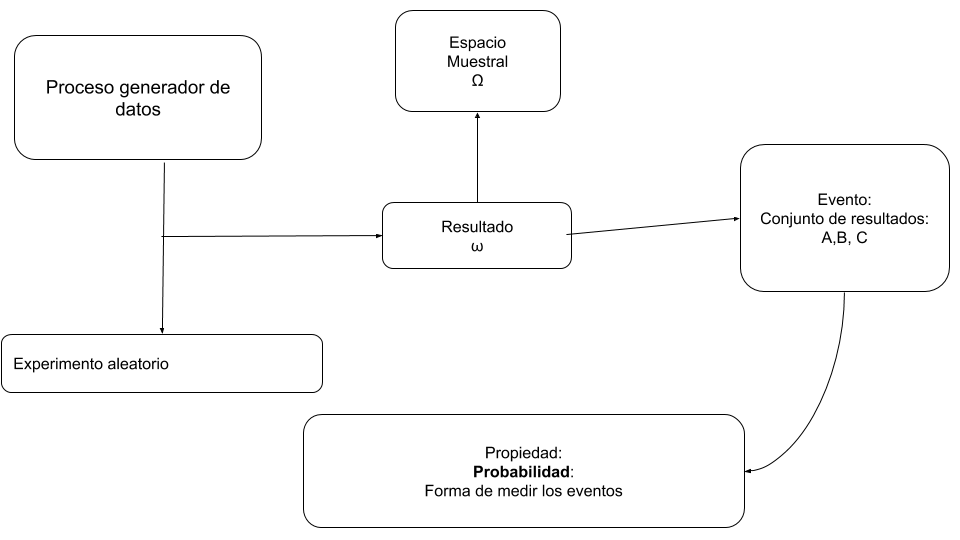
\includegraphics[width=10.41667in,height=\textheight]{img/marco_proba.png}

\begin{itemize}
\tightlist
\item
  El análisis de las probabilidades parte de un \textbf{proceso generador de datos} entendido como cualquier fenómeno que produce algún tipo de información de forma sistemática.
\item
  Cada iteración de este proceso produce información, que podemos interpretar como un \textbf{resultado}.
\item
  Existe un conjunto de posibles resultados, que definimos como \textbf{espacio muestral}.
\item
  Un \textbf{evento} es el conjunto de resultados ocurridos.
\item
  En este marco, la \textbf{probabilidad} es un atributo de los eventos. Es la forma de medir los eventos tal que, siguiendo la definición moderna de probabilidad:
\end{itemize}

\begin{enumerate}
\def\labelenumi{\Alph{enumi})}
\tightlist
\item
  \(P(A) \geq 0 \forall \ A \subseteq \Omega\)
\item
  \(P(\Omega)=1\)
\item
  \(P(A\cup B) = P(A) + P(B)\ si\ A \cap B = \emptyset\)
\end{enumerate}

\begin{quote}
ejemplo, tiramos un dado y sale tres
\end{quote}

\begin{itemize}
\tightlist
\item
  Espacio muestral: 1,2,3,4,5,6
\item
  Restulado: 3
\item
  Evento: impar (el conjunto 1,3,5)
\end{itemize}

\hypertarget{distribucion-de-probabilidad}{%
\subsubsection{Distribución de probabilidad}\label{distribucion-de-probabilidad}}

\begin{itemize}
\item
  La distribución de probabilidad hace referencia a los posibles valores teóricos de cada uno de los resultados pertenecientes al espacio muestral.
\item
  Existen dos tipos de distribuciones, dependiendo si el espacio muestral es o no numerable.
\end{itemize}

\hypertarget{distribuciones-discretas}{%
\paragraph{Distribuciones discretas}\label{distribuciones-discretas}}

Sigamos con el ejemplo de dado.

Podríamos definir la distribución de probabilidad, si no esta cargado, cómo:

\begin{verbatim}
## # A tibble: 6 x 2
##   valor probabilidad
##   <int> <chr>       
## 1     1 1/6         
## 2     2 1/6         
## 3     3 1/6         
## 4     4 1/6         
## 5     5 1/6         
## 6     6 1/6
\end{verbatim}

Cómo el conjunto de resultados posibles es acotado, podemos definirlo en una tabla, esta es una distribución \emph{discreta}

\hypertarget{distribuciones-continuas}{%
\paragraph{Distribuciones continuas}\label{distribuciones-continuas}}

¿Qué pasa cuando el conjunto de resultados posibles es tan grande que no se puede enumerar la probabilidad de cada caso?

Si, por definición o por practicidad, no se puede ennumerar cada caso, lo que tenemos es una \textbf{distribución continua}

\begin{quote}
Por ejemplo, la altura de la población
\end{quote}

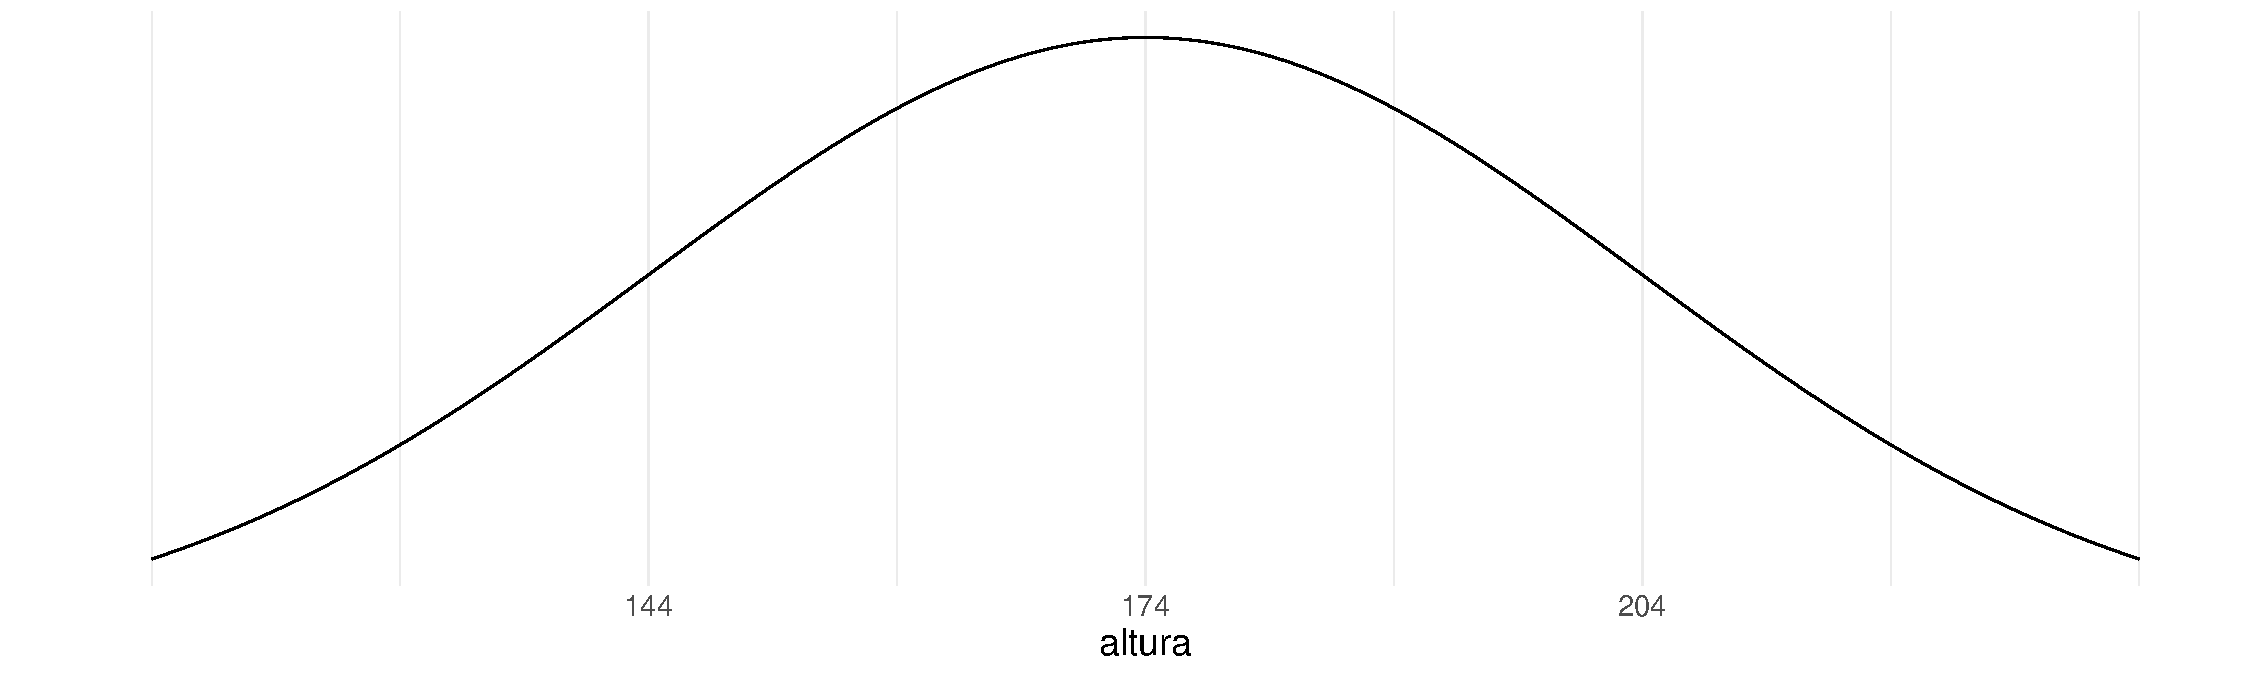
\includegraphics{bookdown_files/figure-latex/unnamed-chunk-33-1.pdf}

\begin{itemize}
\item
  En este caso, no podemos definir en una tabla la probabilidad de cada uno de los posibles valores. \emph{de hecho, la probabilidad puntual es 0}.
\item
  Sin embargo, sí pódemos definir una \emph{función de probabilidad}, la \emph{densidad}.
\item
  Según qué función utilicemos, cambiara la forma de la curva.
\end{itemize}

Por ejemplo:

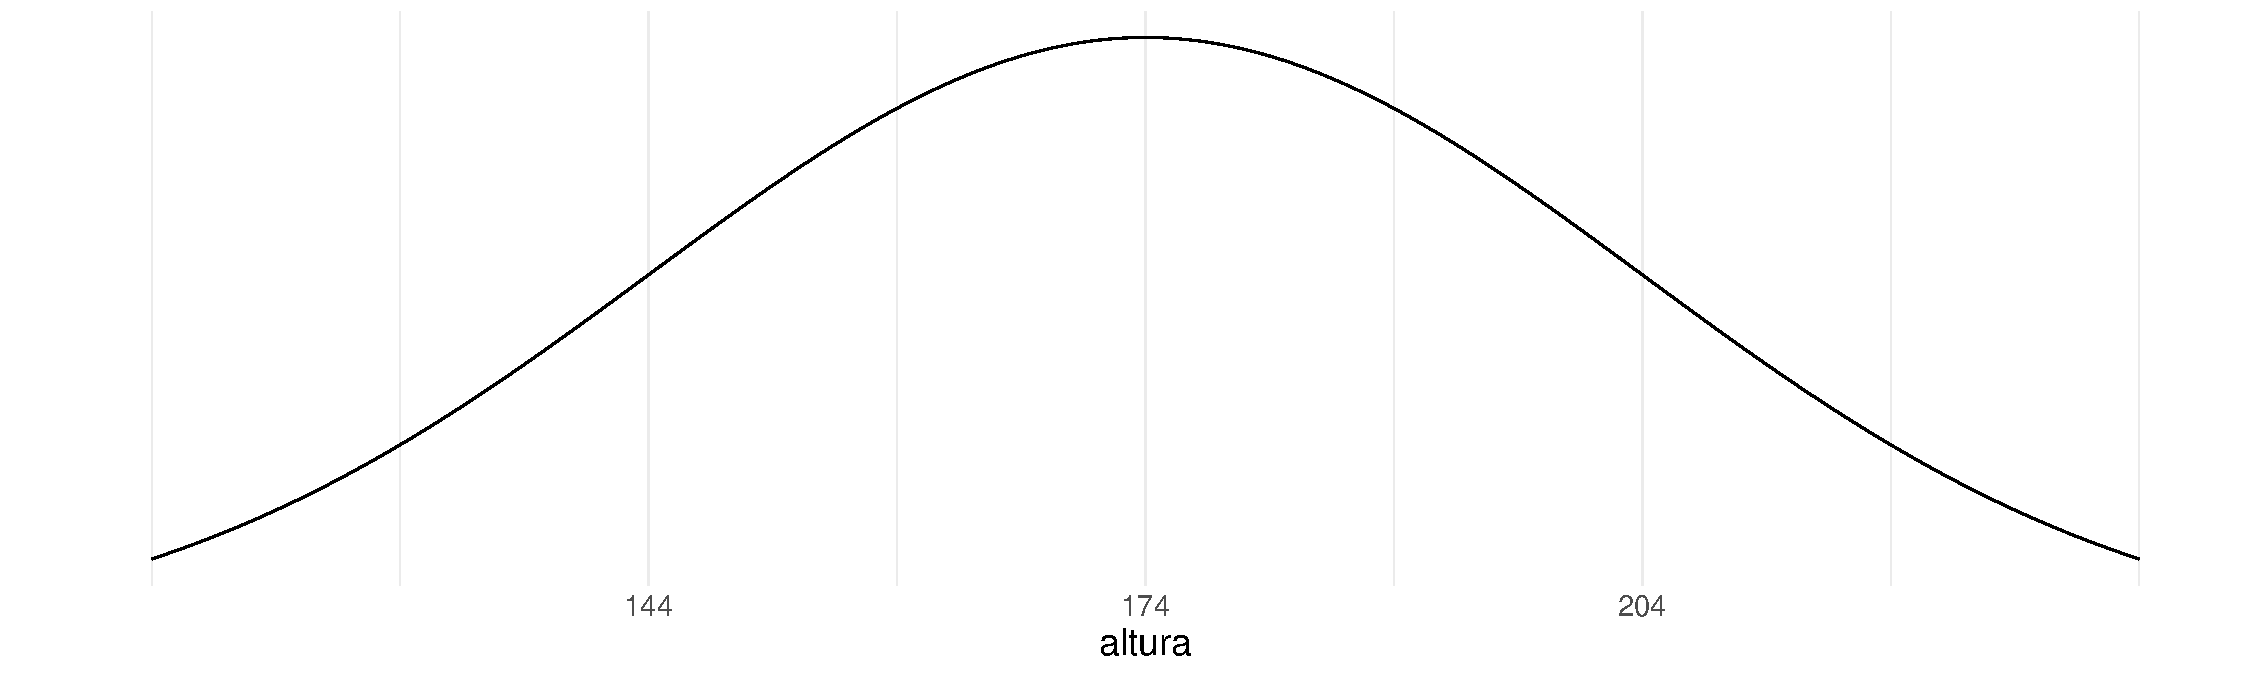
\includegraphics{bookdown_files/figure-latex/unnamed-chunk-34-1.pdf} 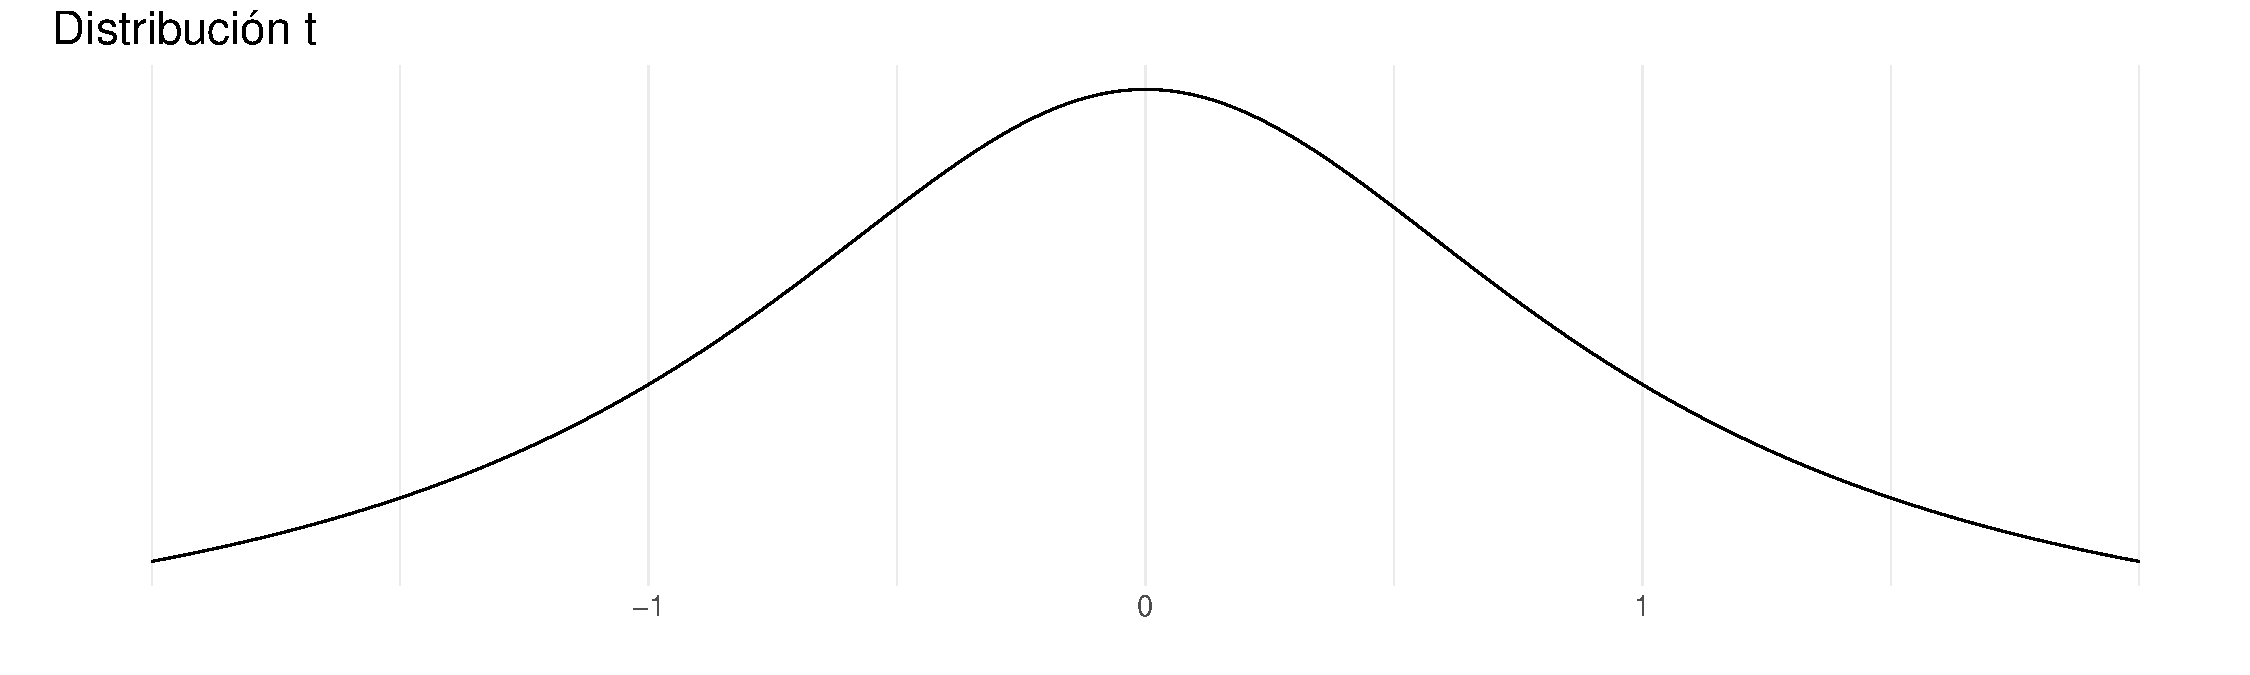
\includegraphics{bookdown_files/figure-latex/unnamed-chunk-34-2.pdf} 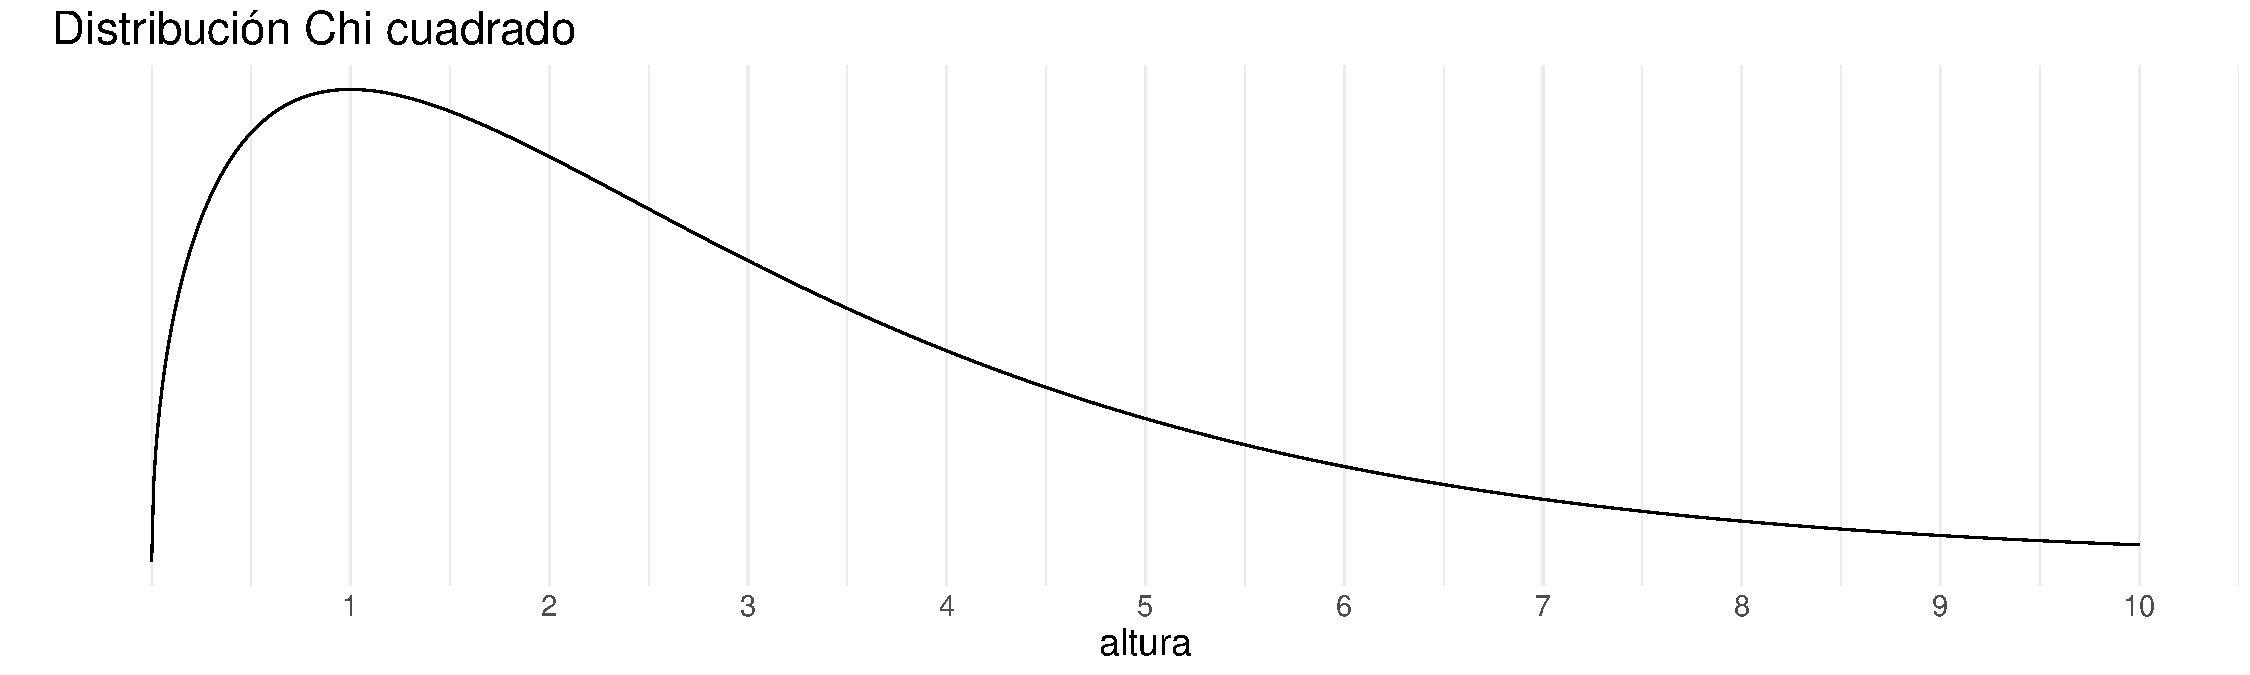
\includegraphics{bookdown_files/figure-latex/unnamed-chunk-34-3.pdf}

\begin{quote}
Una distribución de probabilidad se \textbf{caracteriza} por sus \emph{parámetros}.
\end{quote}

\begin{itemize}
\tightlist
\item
  Por ejemplo, la distribución normal se caracteriza por su \emph{esperanza} y su \emph{varianza} (o desvío estándar)
\end{itemize}

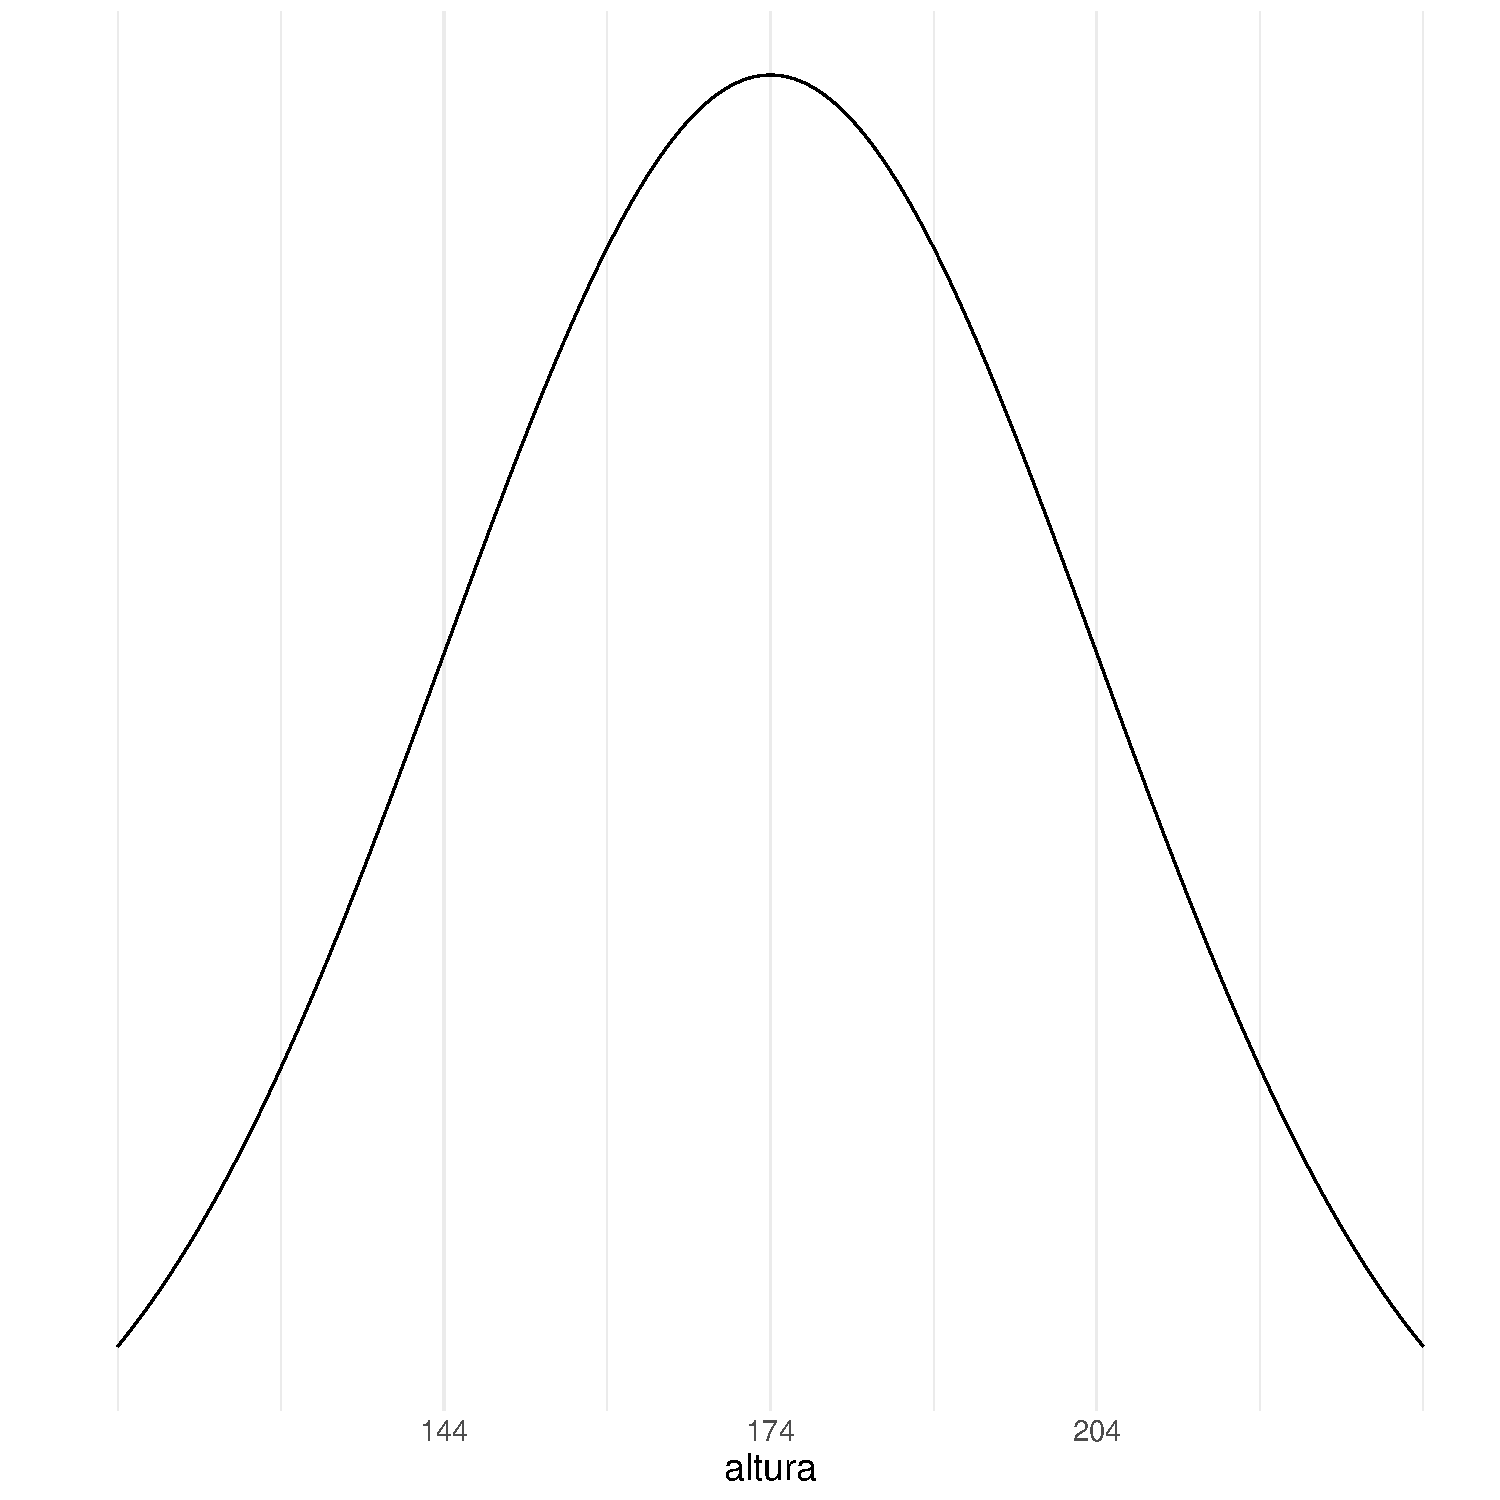
\includegraphics{bookdown_files/figure-latex/unnamed-chunk-35-1.pdf} 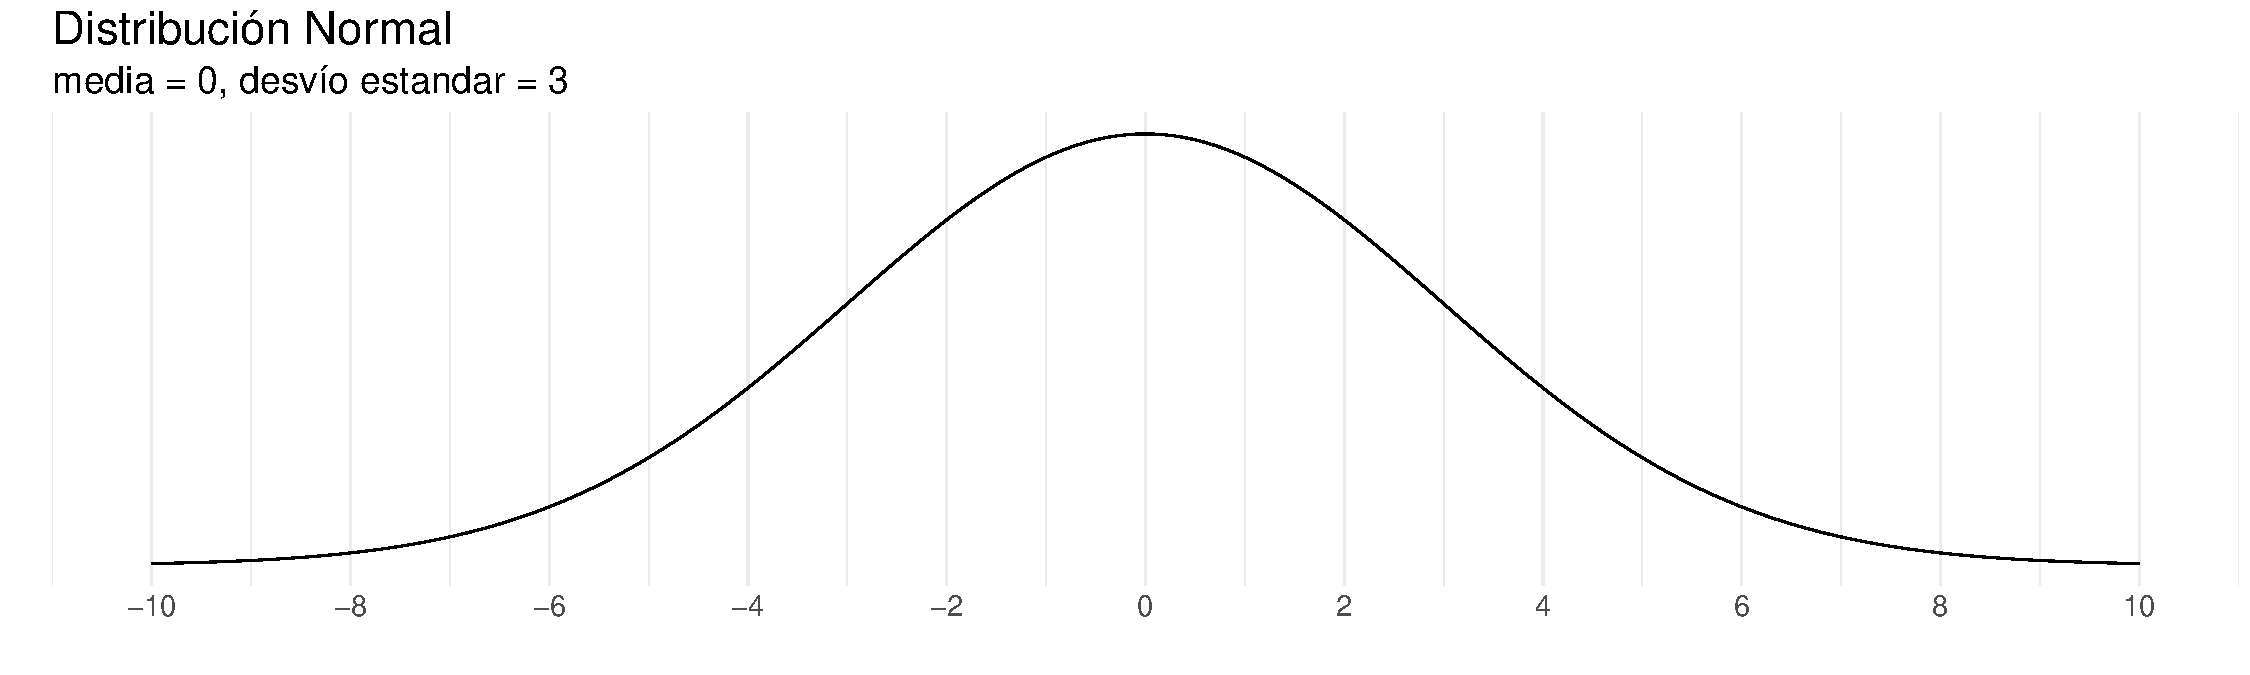
\includegraphics{bookdown_files/figure-latex/unnamed-chunk-35-2.pdf} 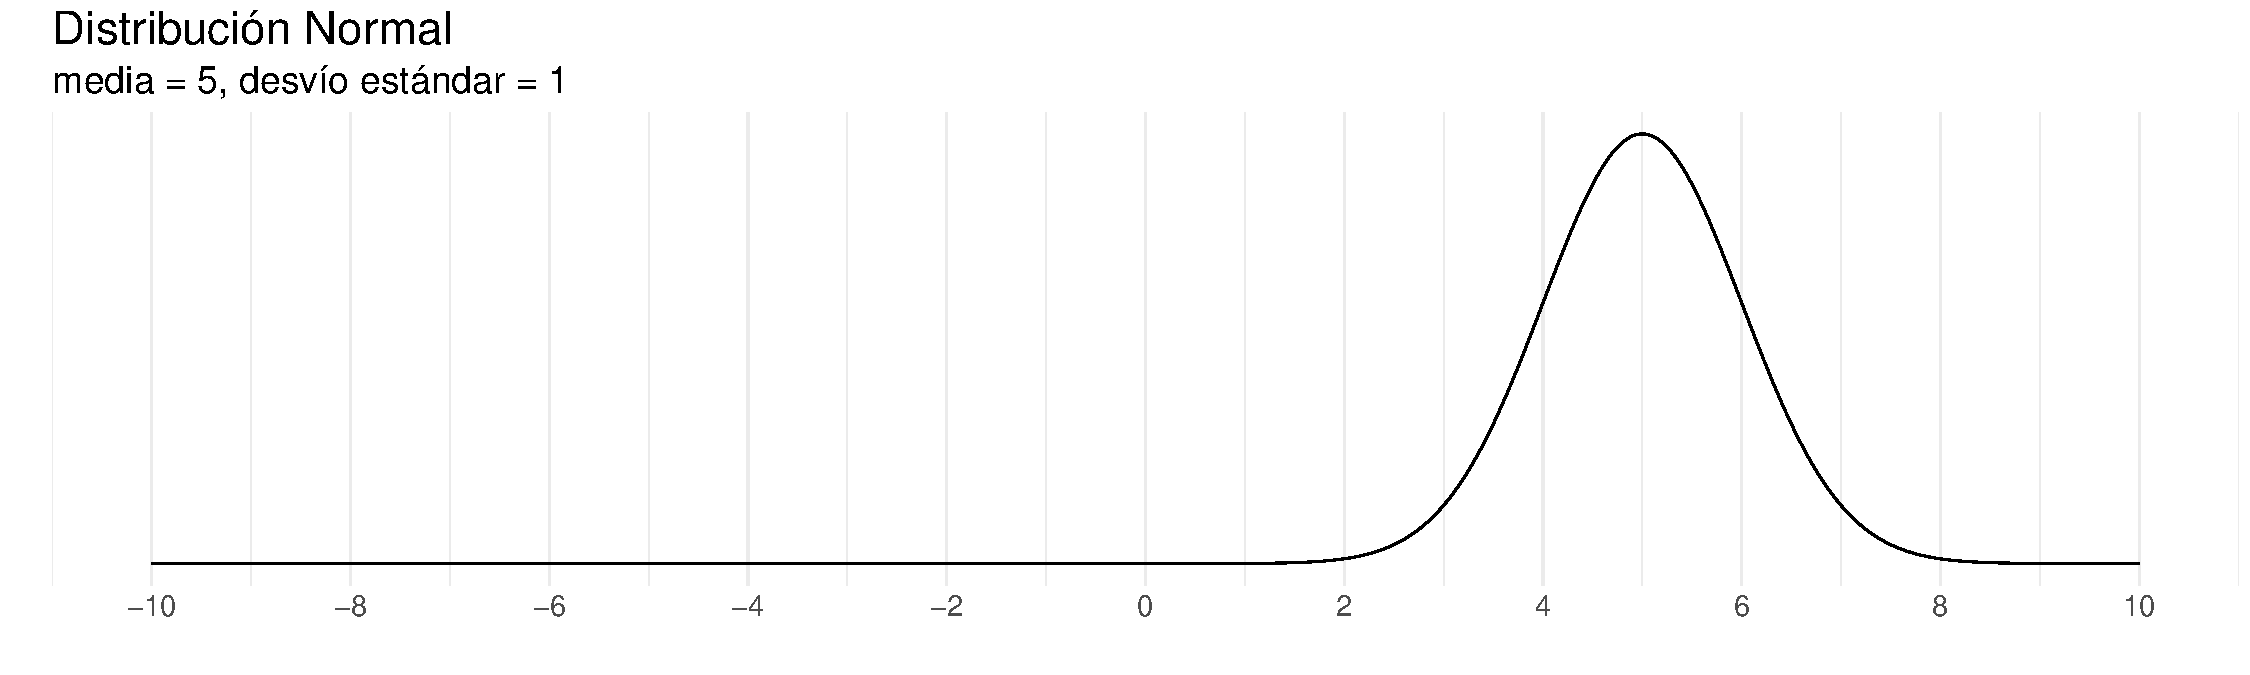
\includegraphics{bookdown_files/figure-latex/unnamed-chunk-35-3.pdf}

\hypertarget{estadistica}{%
\subsection{Estadística}\label{estadistica}}

\hypertarget{el-problema-de-la-inversion}{%
\subsubsection{El problema de la inversión}\label{el-problema-de-la-inversion}}

El problema de la probabilidad se podría pensar de la siguiente forma:

\begin{enumerate}
\def\labelenumi{\arabic{enumi}.}
\tightlist
\item
  Vamos a partir de un \textbf{proceso generador de datos}
\item
  para calcular su \textbf{distribución de probabilidad}, los \textbf{parámetros} que caracterizan a ésta, y a partir de allí,
\item
  calcular la probabilidad de que, al tomar una \textbf{muestra}, tenga ciertos eventos.
\end{enumerate}

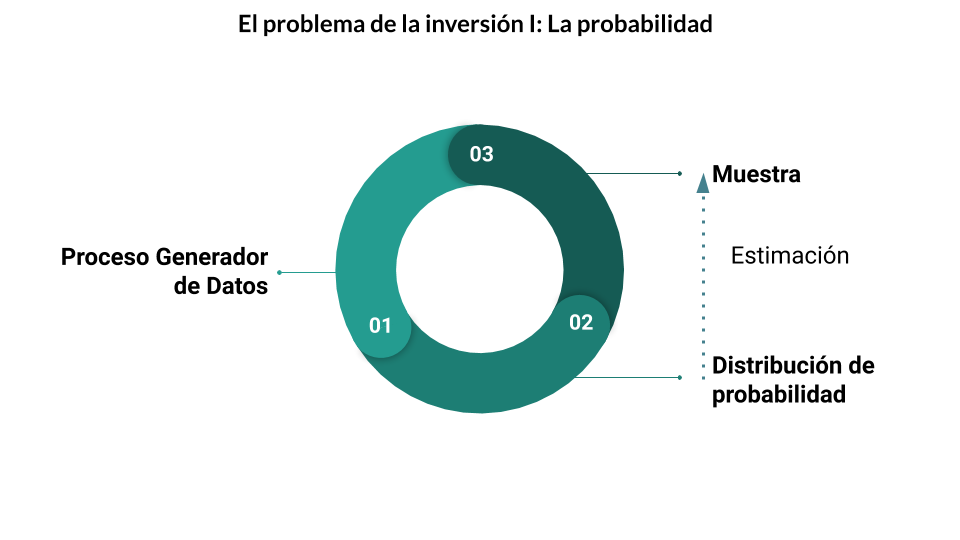
\includegraphics[width=10.41667in,height=\textheight]{img/problema_inversion_1.png}

El problema de la estadística es exactamente el contrario:

\begin{enumerate}
\def\labelenumi{\arabic{enumi}.}
\tightlist
\item
  Partimos de una \textbf{muestra} para
\item
  inferir cuál es la \textbf{distribución de probabilidad}, y los \textbf{parámetros} que la caracterizan
\item
  para finalmente poder sacar conclusiones sobre el \textbf{proceso generador de datos}
\end{enumerate}

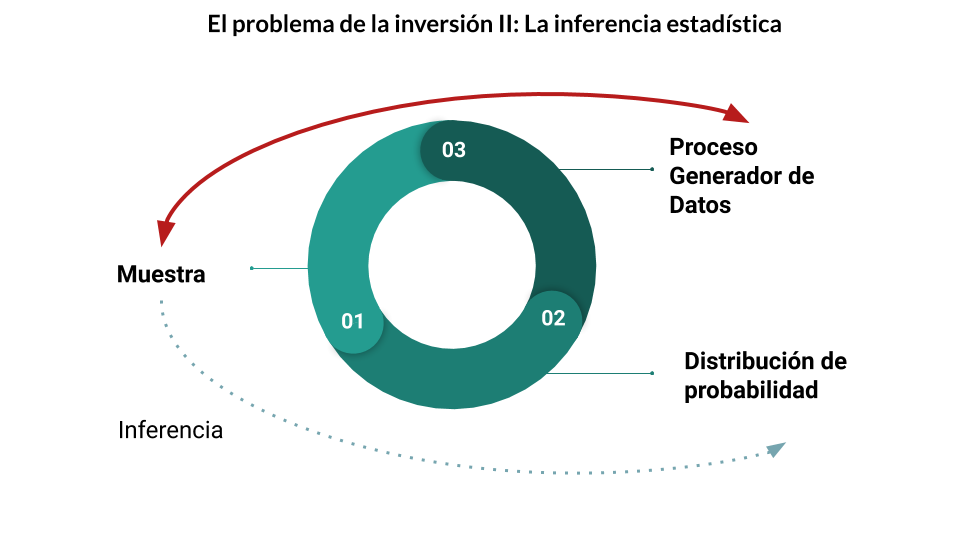
\includegraphics[width=10.41667in,height=\textheight]{img/problema_inversion_2.png}

\hypertarget{poblacion-y-muestra}{%
\paragraph{Población y muestra}\label{poblacion-y-muestra}}

En este punto podemos hacer la distinción entre \textbf{población} y \textbf{muestra}

\begin{itemize}
\tightlist
\item
  \textbf{Población}: El universo en estudio. Puede ser:

  \begin{itemize}
  \tightlist
  \item
    finita: Los votantes en una elección.
  \item
    infinita: El lanzamiento de una moneda.
  \end{itemize}
\item
  \textbf{Muestra}: subconjunto de n observaciones de una población.
\end{itemize}

Solemos utilizar las mayúsculas (N) para la población y las minúsculas (n) para las muestras

\hypertarget{parametros-y-estimadores}{%
\paragraph{Parámetros y Estimadores}\label{parametros-y-estimadores}}

\begin{itemize}
\tightlist
\item
  Como dijimos, los \textbf{parámetros} describen a la función de probabilidad. Por lo tanto hacen referencia a los atributos de la \textbf{población}. Podemos suponer que son \emph{constantes}
\item
  Un \textbf{estimador} es un estadístico (esto es, una función de la muestra) usado para estimar un parámetro desconocido de la población.
\end{itemize}

\hypertarget{ejemplo.-la-media}{%
\paragraph{Ejemplo. La media}\label{ejemplo.-la-media}}

Esperanza o Media Poblacional:

\[
\mu = E(x)= \sum_{i=1}^N x_ip(x_i)
\]

Media muestral:

\[
\bar{X}= \sum_{i=1}^n \frac{Xi}{n}
\]

Como no puedo conocer \(\mu\), lo estimo mediante \(\bar{X}\)

\hypertarget{estimacion-puntual-intervalos-de-confianza-y-tests-de-hipotesis}{%
\subsubsection{Estimación puntual, Intervalos de confianza y Tests de hipótesis}\label{estimacion-puntual-intervalos-de-confianza-y-tests-de-hipotesis}}

\begin{itemize}
\item
  El estimador \(\bar{X}\) nos devuelve un número. Esto es una inferencia de cuál creemos que es la media. Pero no es seguro de que esa sea realmente la media. Esto es lo que denominamos estimación puntual
\item
  También podemos estimar un intervalo, dentro del cual consideramos que se encuentra la media poblacional. La ventaja de esta metodología es que podemos definir la probabilidad de que el parametro poblacional realmente este dentro de este intervalo. Esto se conoce como \textbf{intervalos de confianza}
\item
  Por su parte, también podemos calcular la probabilidad de que el parámetro poblacional sea mayor, menor o igual a un cierto valor. Esto es lo que se conoce como \textbf{test de hipótesis}.
\item
  En el fondo, los intervalos de confianza y los tests de hipótesis se contruyen de igual manera. Son funciones que se construyen a partir de los datos, que se comparan con distribuciones conocidas, \emph{teóricas}.
\end{itemize}

\hypertarget{definicion-de-los-tests}{%
\paragraph{Definición de los tests}\label{definicion-de-los-tests}}

\begin{itemize}
\tightlist
\item
  Los tests se construyen con dos hipótesis: La hipótesis nula \(H_0\), y la hipótesis alternativa, \(H_1\). Lo que buscamos es ver si \emph{hay evidencia suficiente para rechazar la hipótesis nula}.
\end{itemize}

Por ejemplo, si querémos comprobar si la media poblacional, \(\mu\) de una distribución es mayor a \(X_i\), haremos un test con las siguientes hipótesis:

\begin{itemize}
\tightlist
\item
  \(H_0: \mu = X_i\)
\item
  \(H_1: \mu > X_i\)
\end{itemize}

Si la evidencia es lo suficientemente fuerte, podremos rechazar la hipótesis \(H_0\), \emph{pero no afirmar la hipótesis \(H_1\)}

\hypertarget{significatividad-en-los-tests}{%
\paragraph{Significatividad en los tests}\label{significatividad-en-los-tests}}

\begin{itemize}
\item
  Muchas veces decimos que algo es \textbf{``estadísticamente significativo''}. Detras de esto se encuentra un test de hipótesis que indica que hay una suficiente \emph{significativdad estadística}.
\item
  La \emph{significatividad estadística},representada con \(\alpha\), es la probabilidad de rechazar \(H_0\) cuando en realidad es cierta. Por eso, cuanto más bajo el valor de \(\alpha\), más seguros estamos de no equivocarnos. Por lo general testeamos con valores de alpha de 1\%, 5\% y 10\%, dependiendo del área de estudio
\item
  El \textbf{p-valor} es \_la mínima significatividad para la que rechazo el test. Es decir, cuanto más bajo es el p-valor, más seguros estamos de rechazar \(H_0\)
\item
  El resultado de un test esta determinado por

  \begin{enumerate}
  \def\labelenumi{\arabic{enumi}.}
  \tightlist
  \item
    \textbf{La fuerza evidencia empírica}: Si nuestra duda es si la media poblacional es mayor a, digamos, 10. Y la media muestral es 11, no es es lo mismo que si es 100, 1000 o 10000.
  \item
    \textbf{El tamaño de la muestra}: En las fórmulas que definen los test siempre juega el tamaño de la muestra: cuanto más grande es, más seguros estamos de que el resultado no es producto del mero azar.
  \item
    \textbf{La veracidad de los supuestos}: Otra cosa importante es que los test asumen ciertas cosas:
  \end{enumerate}

  \begin{itemize}
  \tightlist
  \item
    Normalidad en los datos.
  \item
    Que conocemos algún otro parámetro de la distribución, como la varianza.
  \item
    Que los datos son independientes entre sí,
  \item
    Etc.\\
    \textbf{Cada Test tiene sus propios supuestos}. Por eso a veces luego de hacer un test, hay que hacer otros tests para validar que los supuestos se cumplen.
  \end{itemize}
\item
  Lo primero, la fuerza de la evidencia, es lo que más nos importa, y no hay mucho por hacer.
\item
  El tamaño de la muestra es un problema, porque si la muesta es muy chica, entonces podemos no llegar a conclusiones significativas aunque sí ocurra aquello que queríamos probar.
\item
  Sin embargo, el verdadero problema en \emph{La era del big data} es que tenemos muestras demasiado grandes, por lo que cualquier test, por más mínima que sea la diferencia, puede dar significativo.
\end{itemize}

\begin{quote}
Por ejemplo, podemos decir que la altura promedio en Argentina es 1,74. Pero si hacemos un test, utilizando como muestra 40 millones de personas, vamos a rechazar que ese es el valor, porque en realidad es 1,74010010. En términos de lo que nos puede interesar, 1,74 sería válido, pero estadísticamente rechazaríamos.
\end{quote}

\begin{itemize}
\tightlist
\item
  Finalmente, según la información que tengamos de la población y cual es el problema que queremos resolver, vamos a tener que utilizar distintos tipos de tests. La cantidad de tests posibles es ENORME, y escapa al contenido de este curso, así como sus fórmulas. A modo de ejemplo, les dejamos el siguiente machete:
\end{itemize}

\begin{figure}
\centering
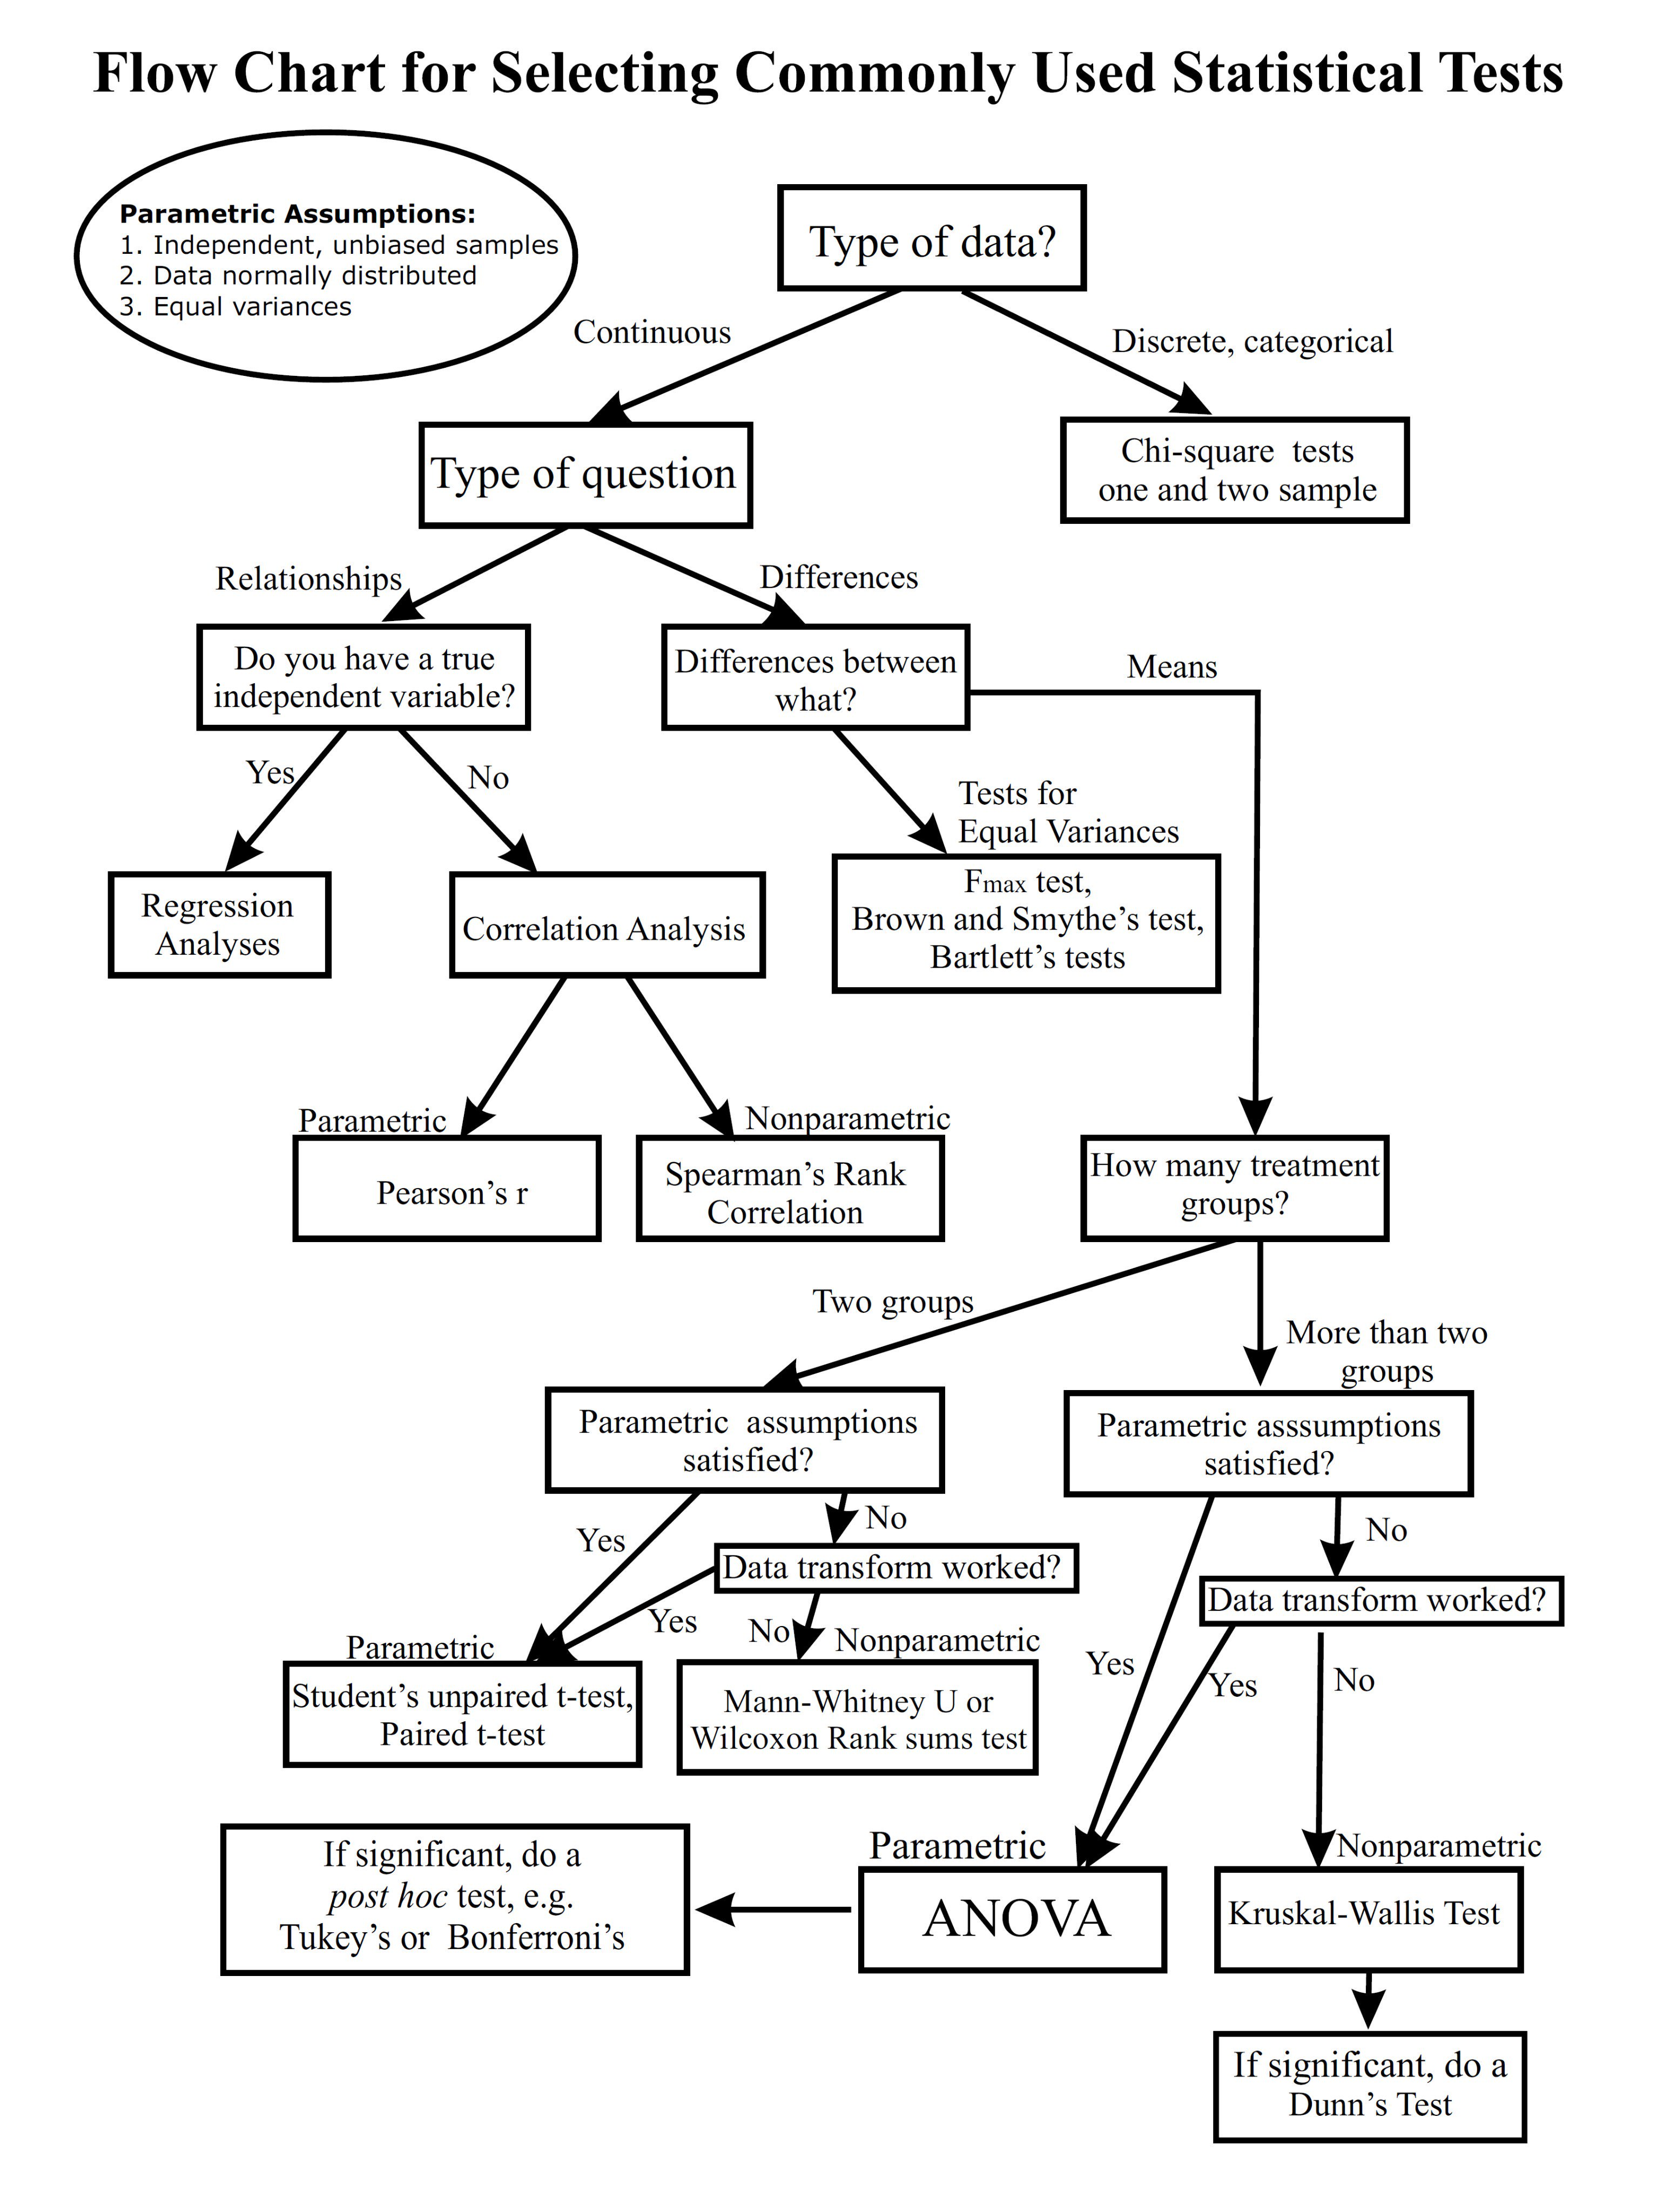
\includegraphics[width=10.41667in,height=\textheight]{img/tests.jpeg}
\caption{fuente: \url{http://abacus.bates.edu/~ganderso/biology/resources/statistics.html}}
\end{figure}

\hypertarget{algunos-estimadores-importantes}{%
\subsection{Algunos estimadores importantes}\label{algunos-estimadores-importantes}}

\hypertarget{medidas-de-centralidad}{%
\subsubsection{Medidas de centralidad}\label{medidas-de-centralidad}}

\begin{itemize}
\tightlist
\item
  \textbf{Media}
\end{itemize}

\[
\bar{X}= \sum_{i=1}^n \frac{Xi}{n}
\]

\begin{itemize}
\tightlist
\item
  \textbf{Mediana}:
\end{itemize}

Es el valor que parte la distribución a la mitad

\begin{itemize}
\tightlist
\item
  \textbf{Moda}
\end{itemize}

La moda es el valor más frecuente de la distribución

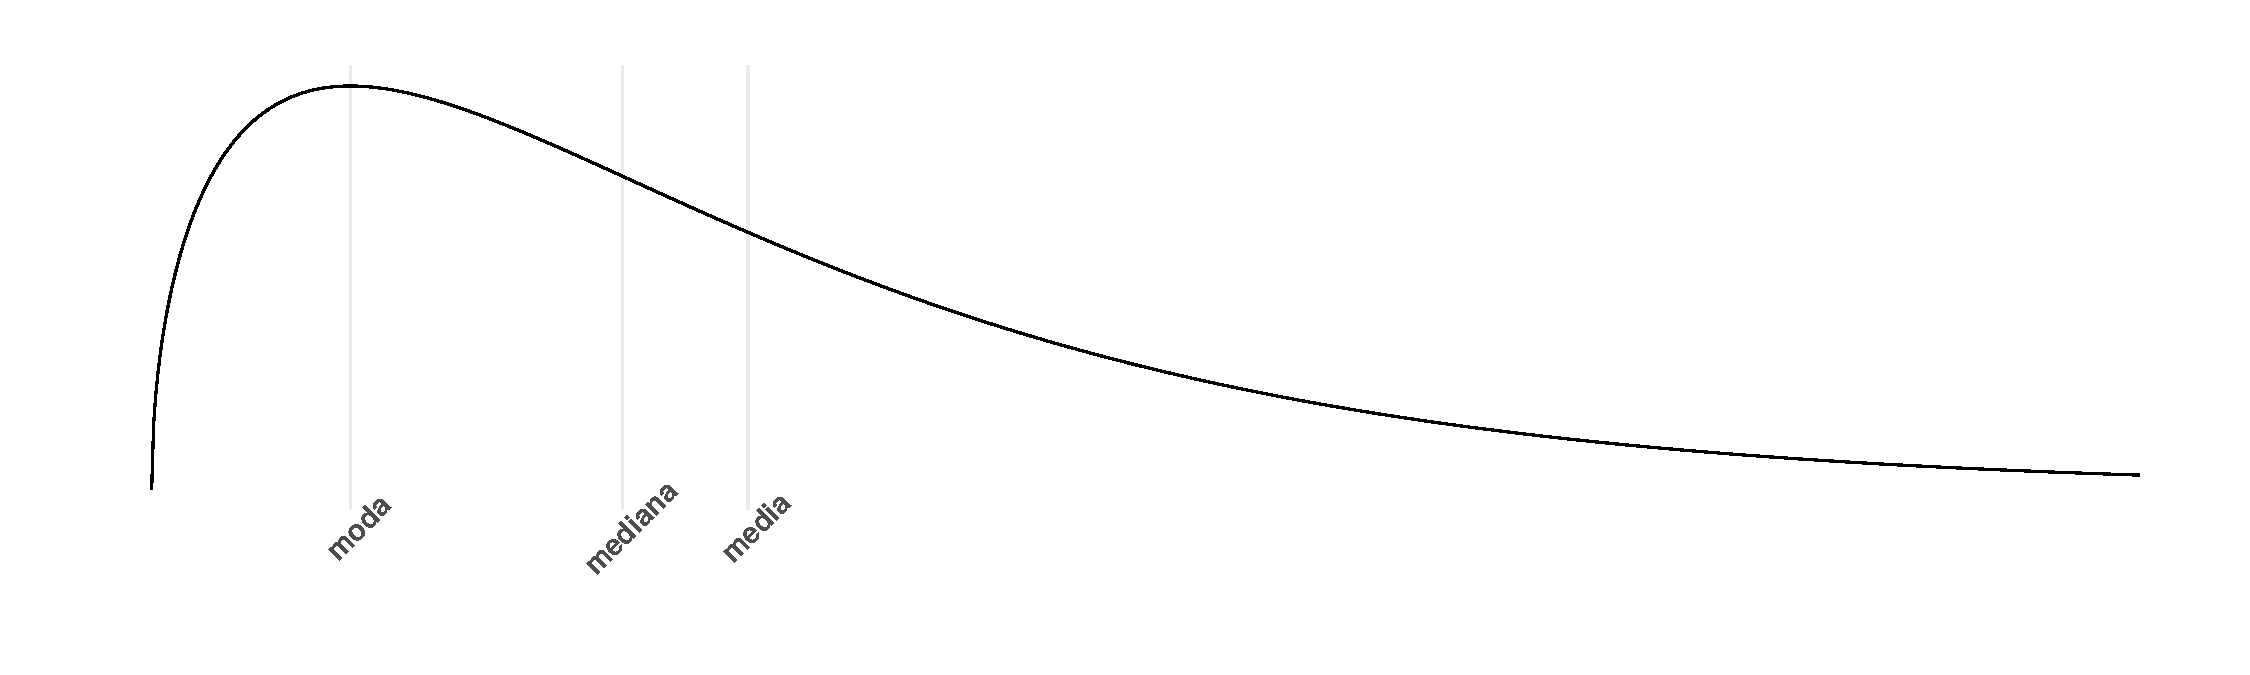
\includegraphics{bookdown_files/figure-latex/unnamed-chunk-36-1.pdf}

\hypertarget{cuantiles}{%
\subsubsection{Cuantiles}\label{cuantiles}}

Así como dijimos que la mediana es el valor que deja al 50\% de los datos de un lado y al 50\% del otro, podemos generalizar este concepto a cualquier X\%. Esto son los cuantiles. El cuantil x, es el valor tal que queda un x\% de la distribución a izquierda, y 1-x a derecha.

Algunos de los más utilizados son el del 25\%, también conocido como \(Q_1\) (el \emph{cuartil} 1), el \(Q_2\) (la mediana) y el \(Q_3\) (el \emph{cuartil} 3), que deja el 75\% de los datos a su derecha. Veamos como se ven en la distribución de arriba

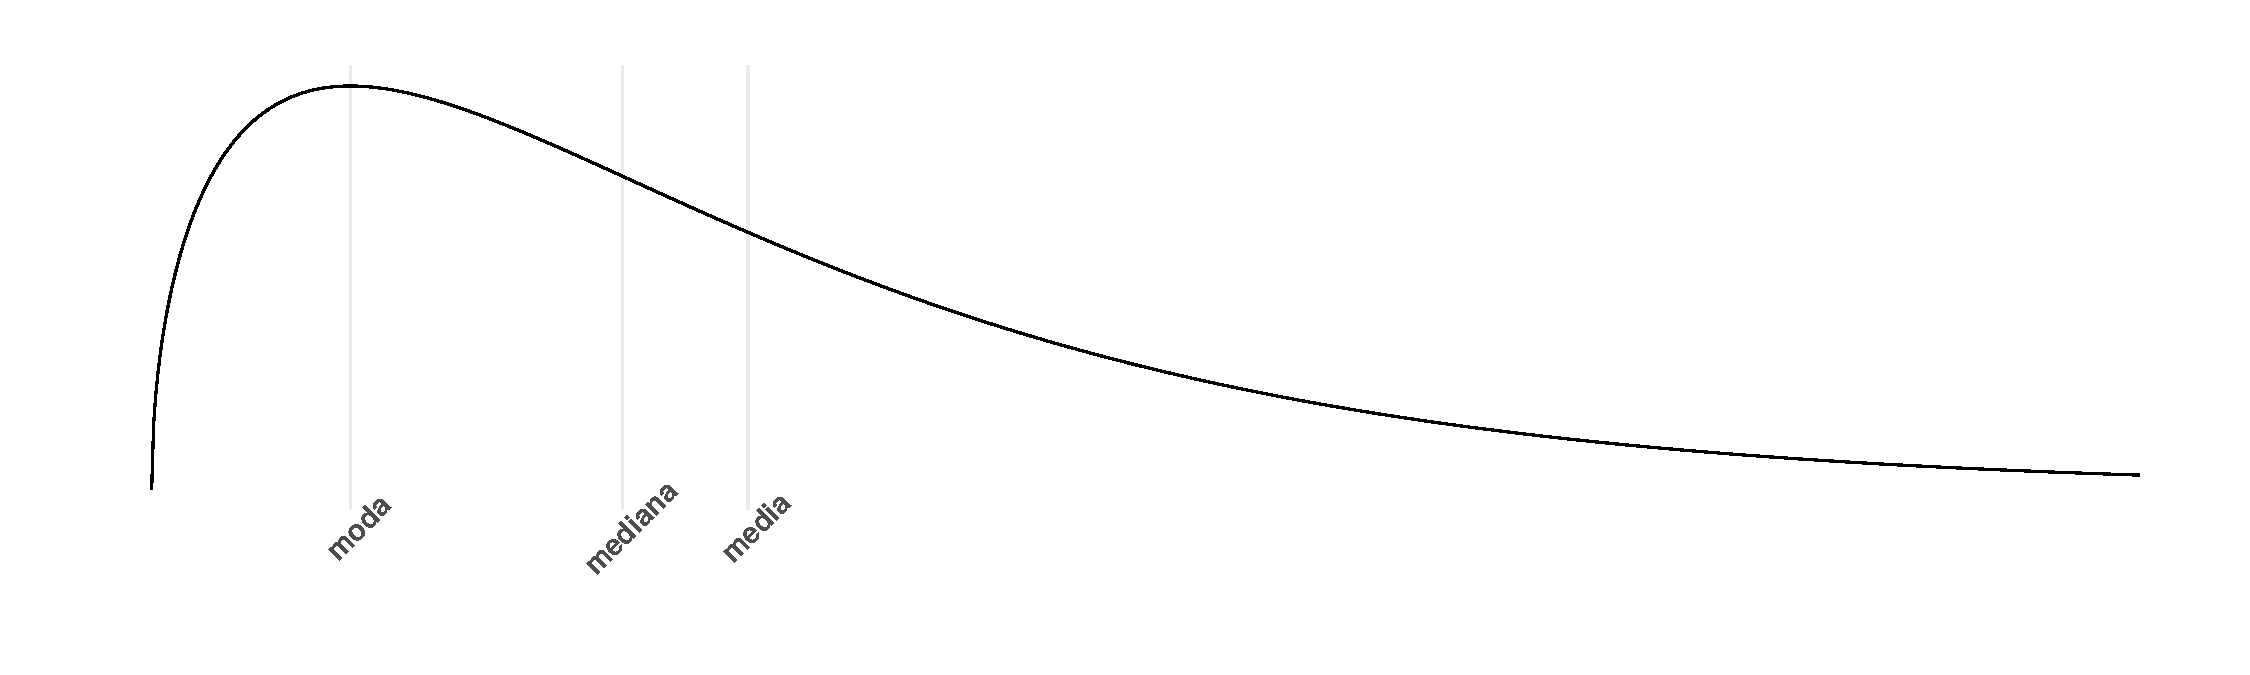
\includegraphics{bookdown_files/figure-latex/unnamed-chunk-37-1.pdf}

\hypertarget{desvio-estandar}{%
\subsubsection{desvío estándar}\label{desvio-estandar}}

\begin{itemize}
\tightlist
\item
  El \emph{desvío estándar} es una medida de dispersión de los datos, que indica cuánto se suelen alejar de la media.
\end{itemize}

\hypertarget{graficos-estadisticos}{%
\subsection{Gráficos estadísticos}\label{graficos-estadisticos}}

Cerramos la explicación con algunos gráficos que resultan útiles para entender las propiedades estadísticas de los datos.

\hypertarget{boxplot}{%
\subsubsection{Boxplot}\label{boxplot}}

El Boxplot es muy útil para describir una distribución y para detectar outliers. Reúne los principales valores que caracterizan a una distribución:

\begin{itemize}
\tightlist
\item
  \(Q_1\)
\item
  \(Q_2\) (la mediana)
\item
  \(Q_3\)
\item
  el \emph{rango intercuarítlico} \(Q_3 - Q_1\), que define el centro de la distribución
\item
  Outliers, definidos como aquellos puntos que se encuentran a más de 1,5 veces el rango intercuartílico del centro de la distribución.
\end{itemize}

veamos qué pinta tienen los boxplot de números generados aleatoriamente a partir de tres distribuciones que ya vimos. En este caso, sólo tomaremos 15 valores de cada distribución

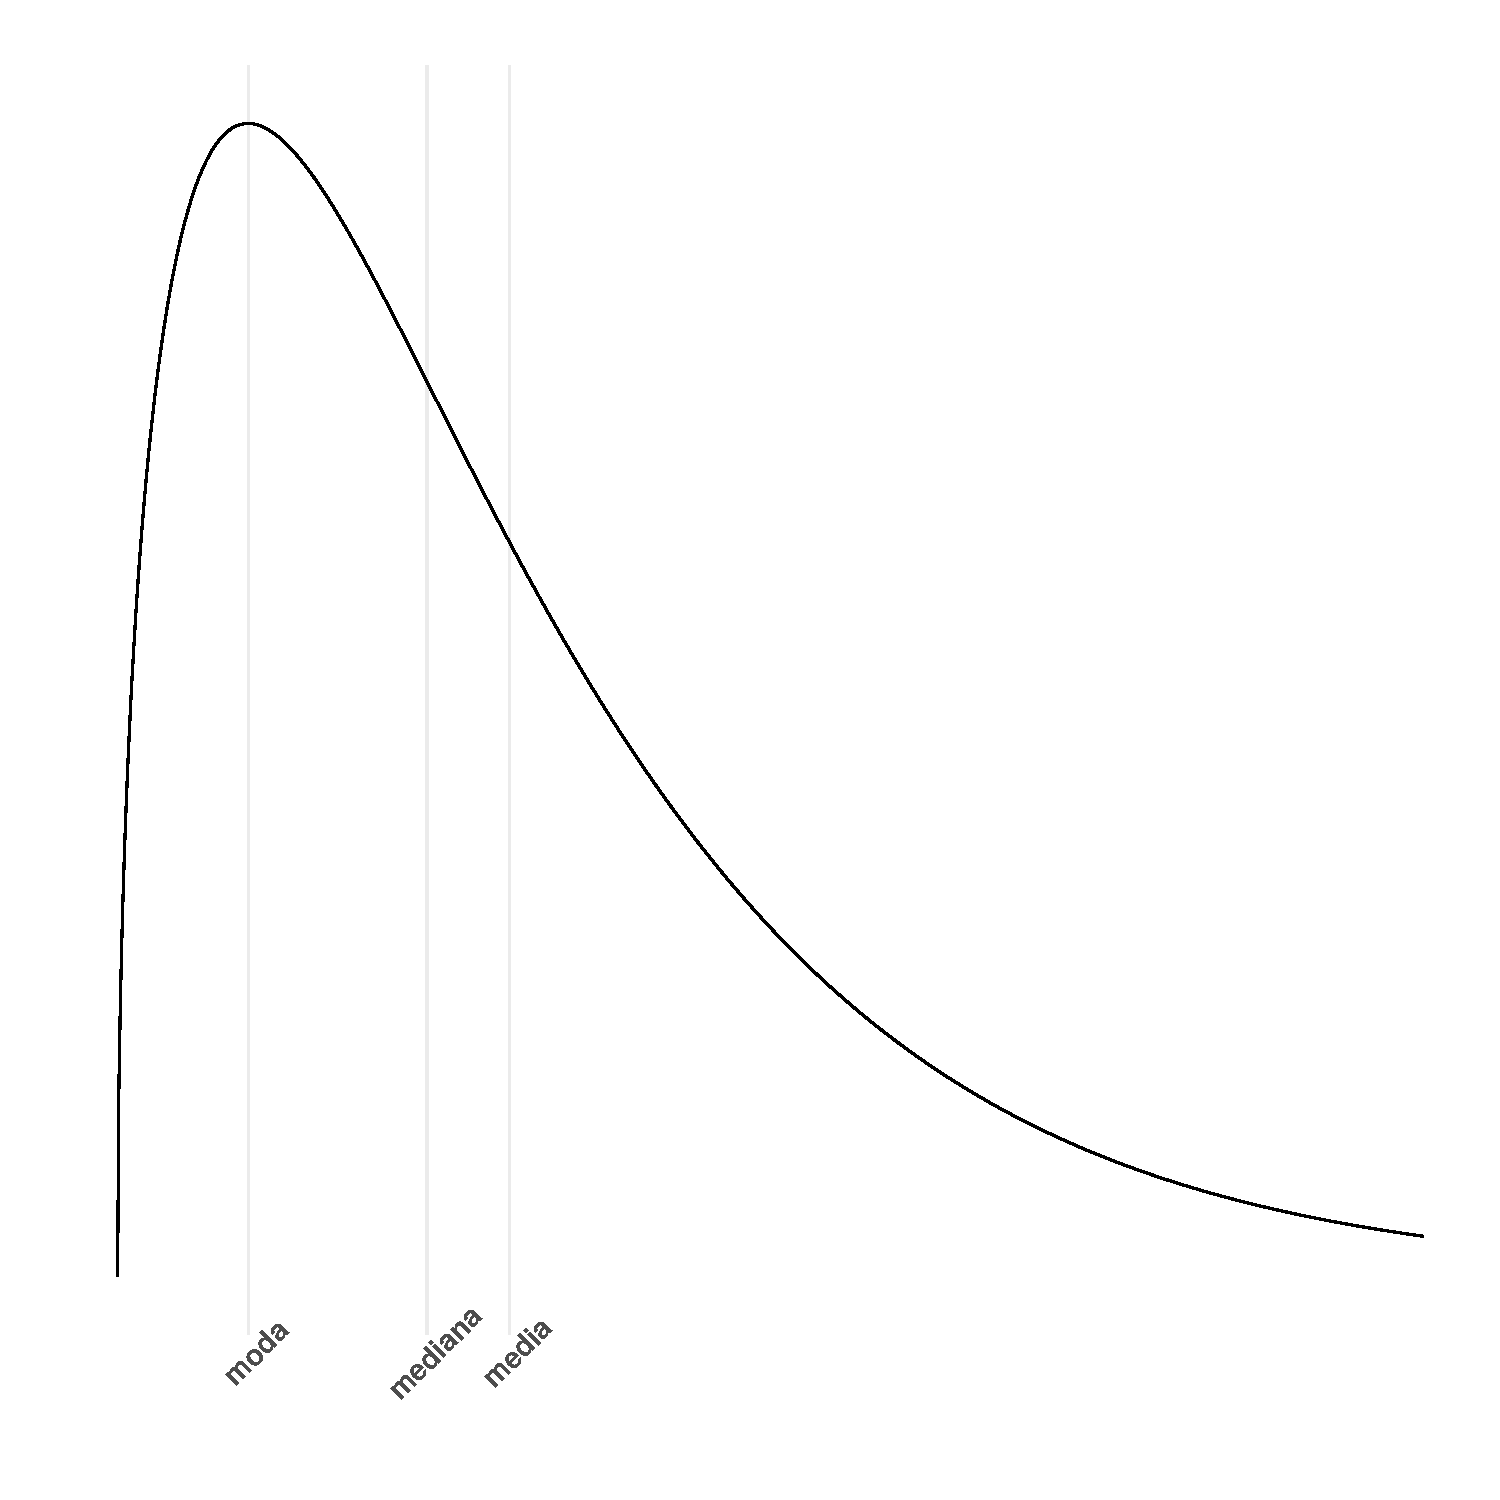
\includegraphics{bookdown_files/figure-latex/unnamed-chunk-38-1.pdf}

Algunas cosas que resaltan:

\begin{itemize}
\tightlist
\item
  la distribución \(\chi^2\) no toma valores en los negativos.
\item
  La normal esta más concentrada en el centro de la distribución
\end{itemize}

Podemos generar 100 números aleatorios en lugar de 15:

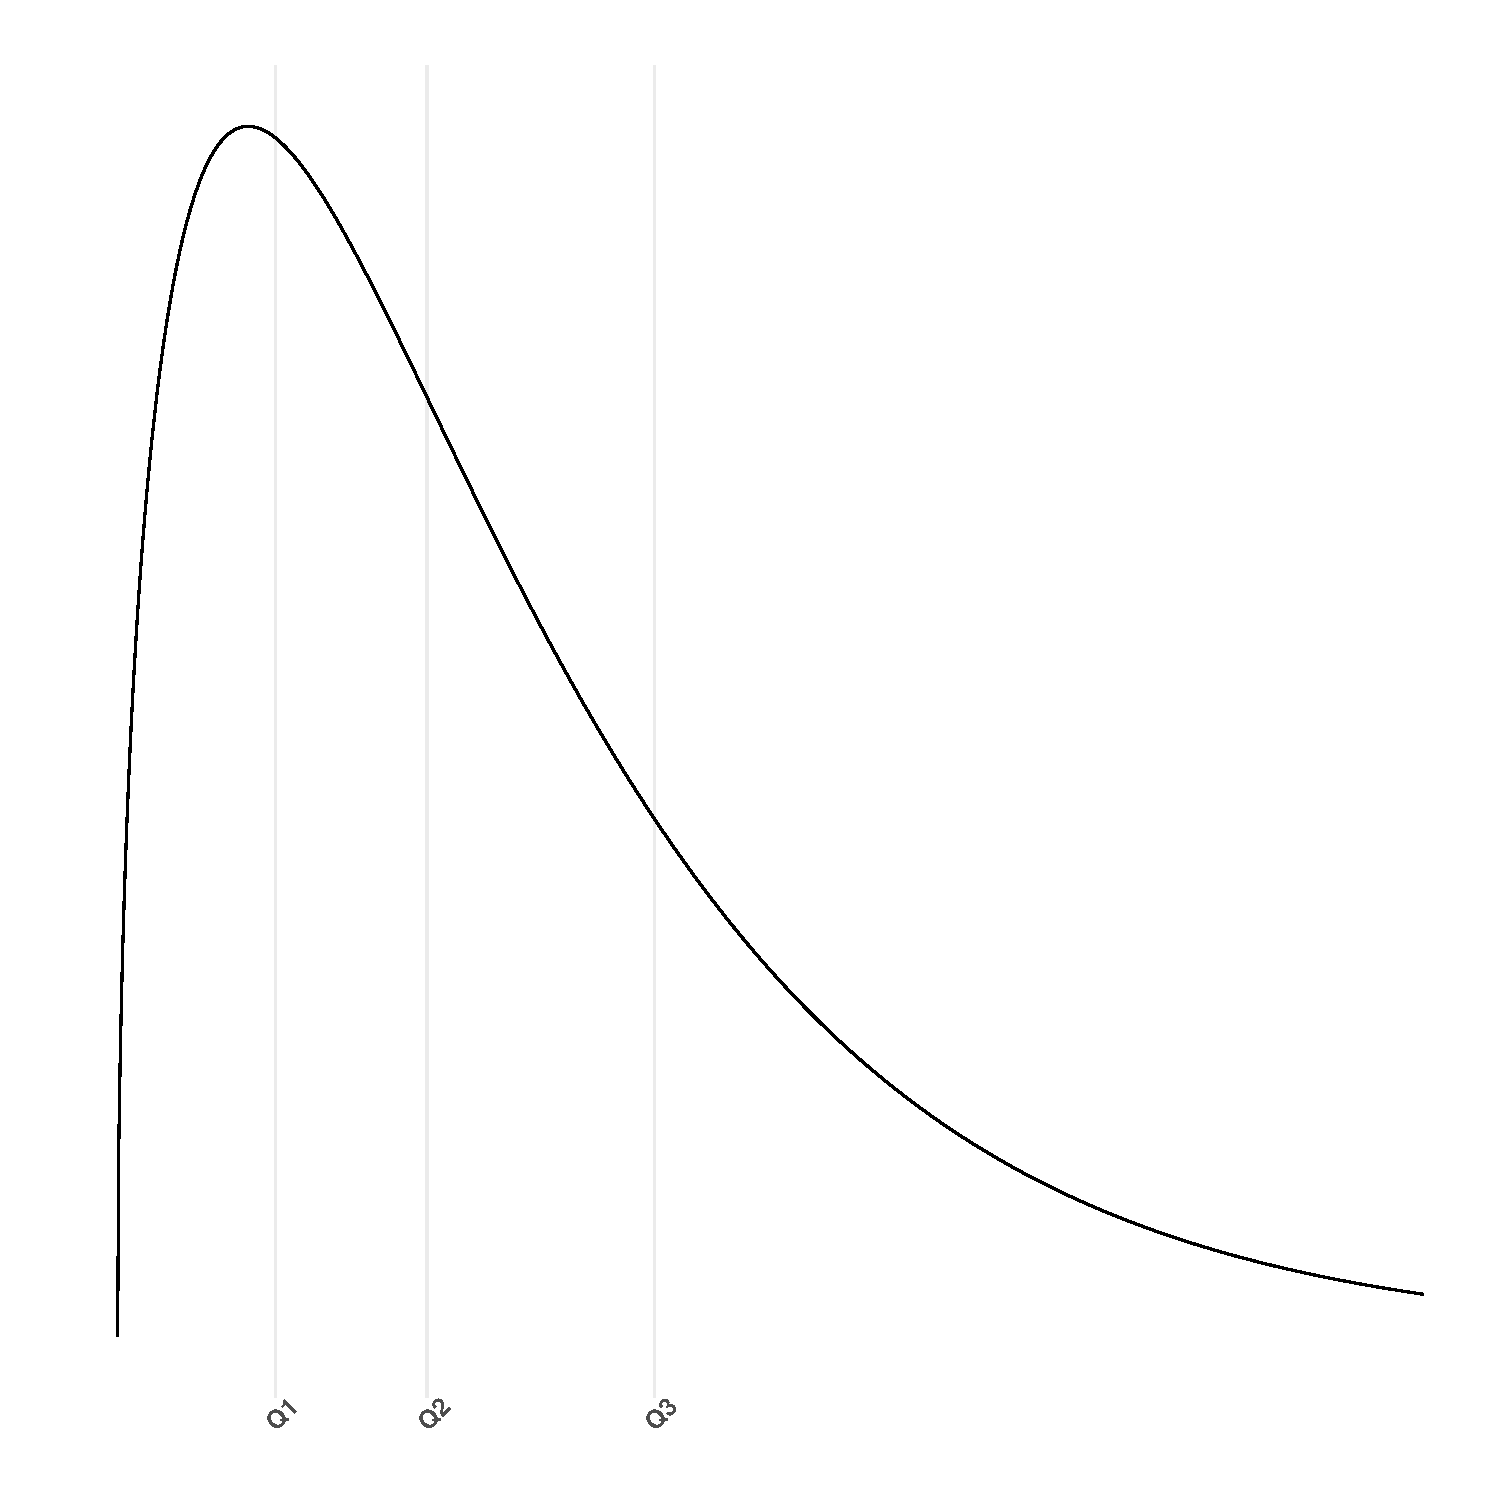
\includegraphics{bookdown_files/figure-latex/unnamed-chunk-39-1.pdf}

Cuando generamos 100 valores en lugar de 15, tenemos más chances de agarrar un punto alejado en la distribución. De esta forma podemos apreciar las diferencias entre la distribución normal y la T-student.

También podemos volver a repasar qué efecto generan los distintos parámetros. Por ejemplo

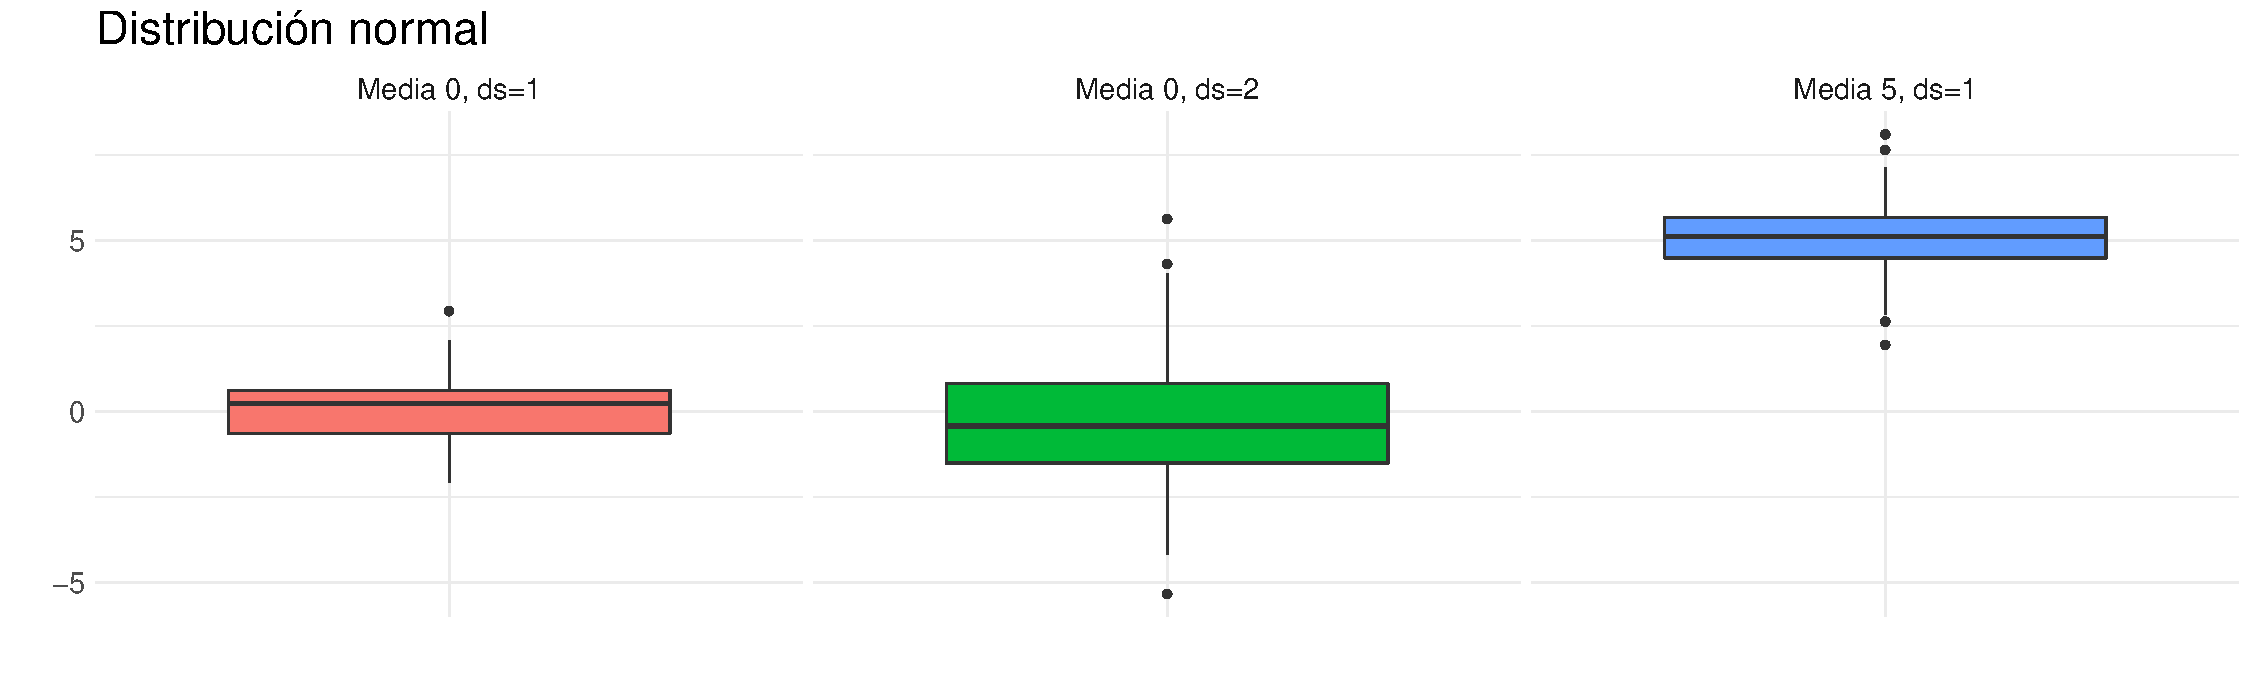
\includegraphics{bookdown_files/figure-latex/unnamed-chunk-40-1.pdf}

\hypertarget{histograma}{%
\subsubsection{Histograma}\label{histograma}}

Otra forma de analizar una distribución es mediante los histogramas:

\begin{itemize}
\tightlist
\item
  En un histograma agrupamos las observaciones en rangos fijos de la variable y contamos la cantidad de ocurrencias.
\item
  Cuanto más alta es una barra, es porque más observaciones se encuentran en dicho rango
\end{itemize}

Veamos el mismo ejemplo que arriba, pero con histogramas

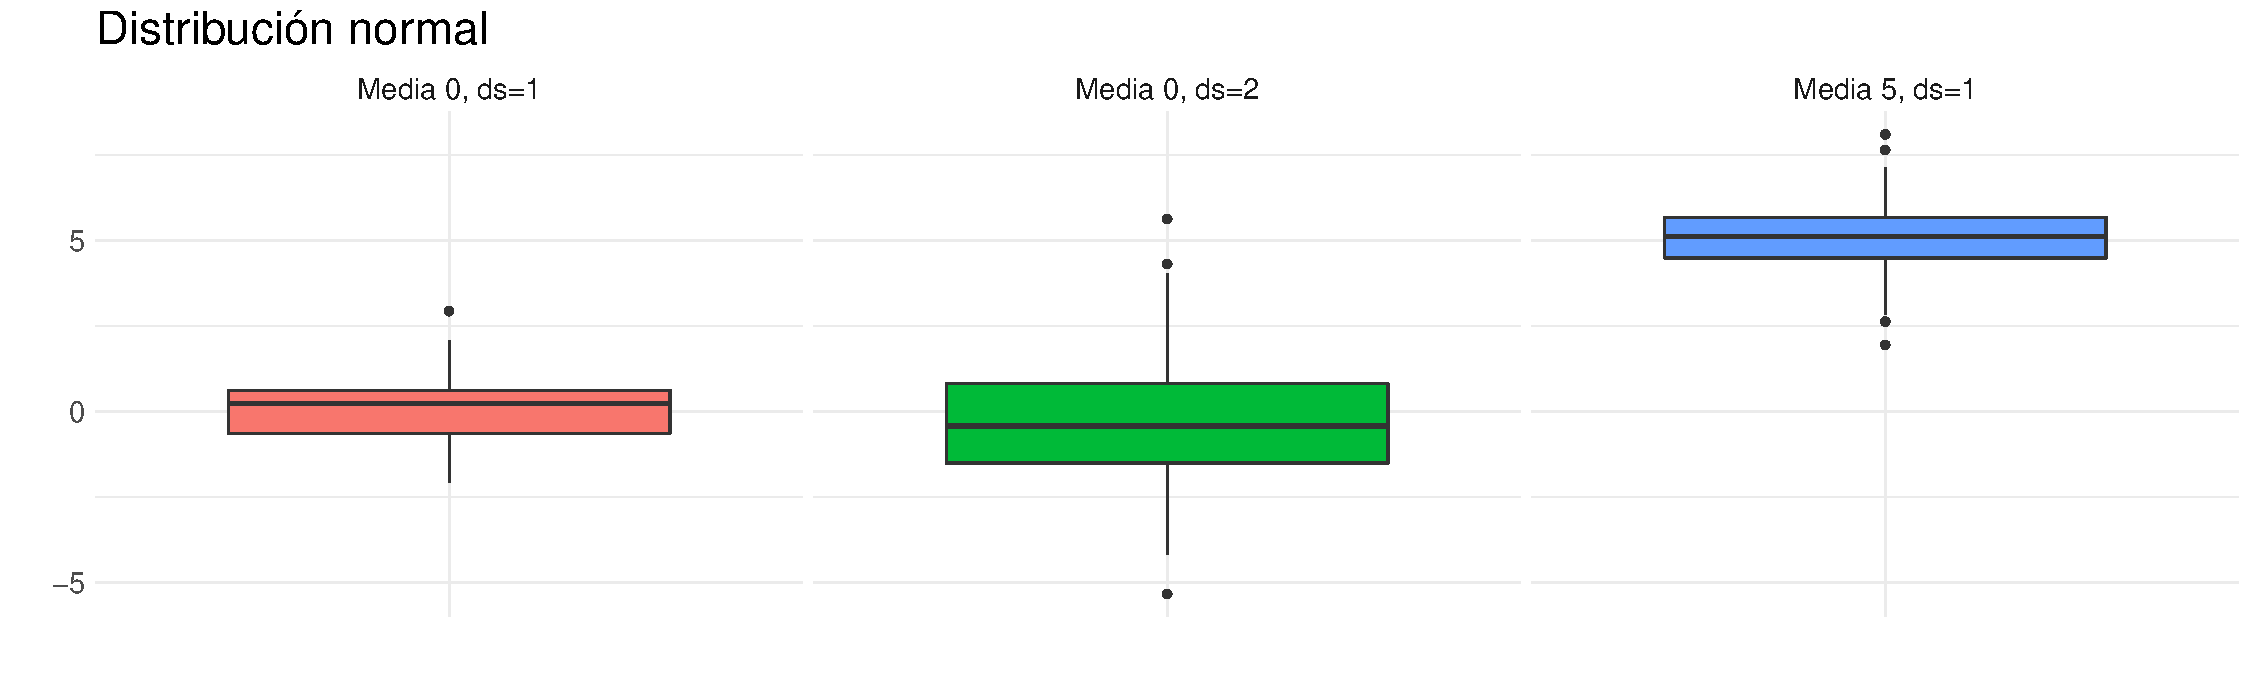
\includegraphics{bookdown_files/figure-latex/unnamed-chunk-41-1.pdf} 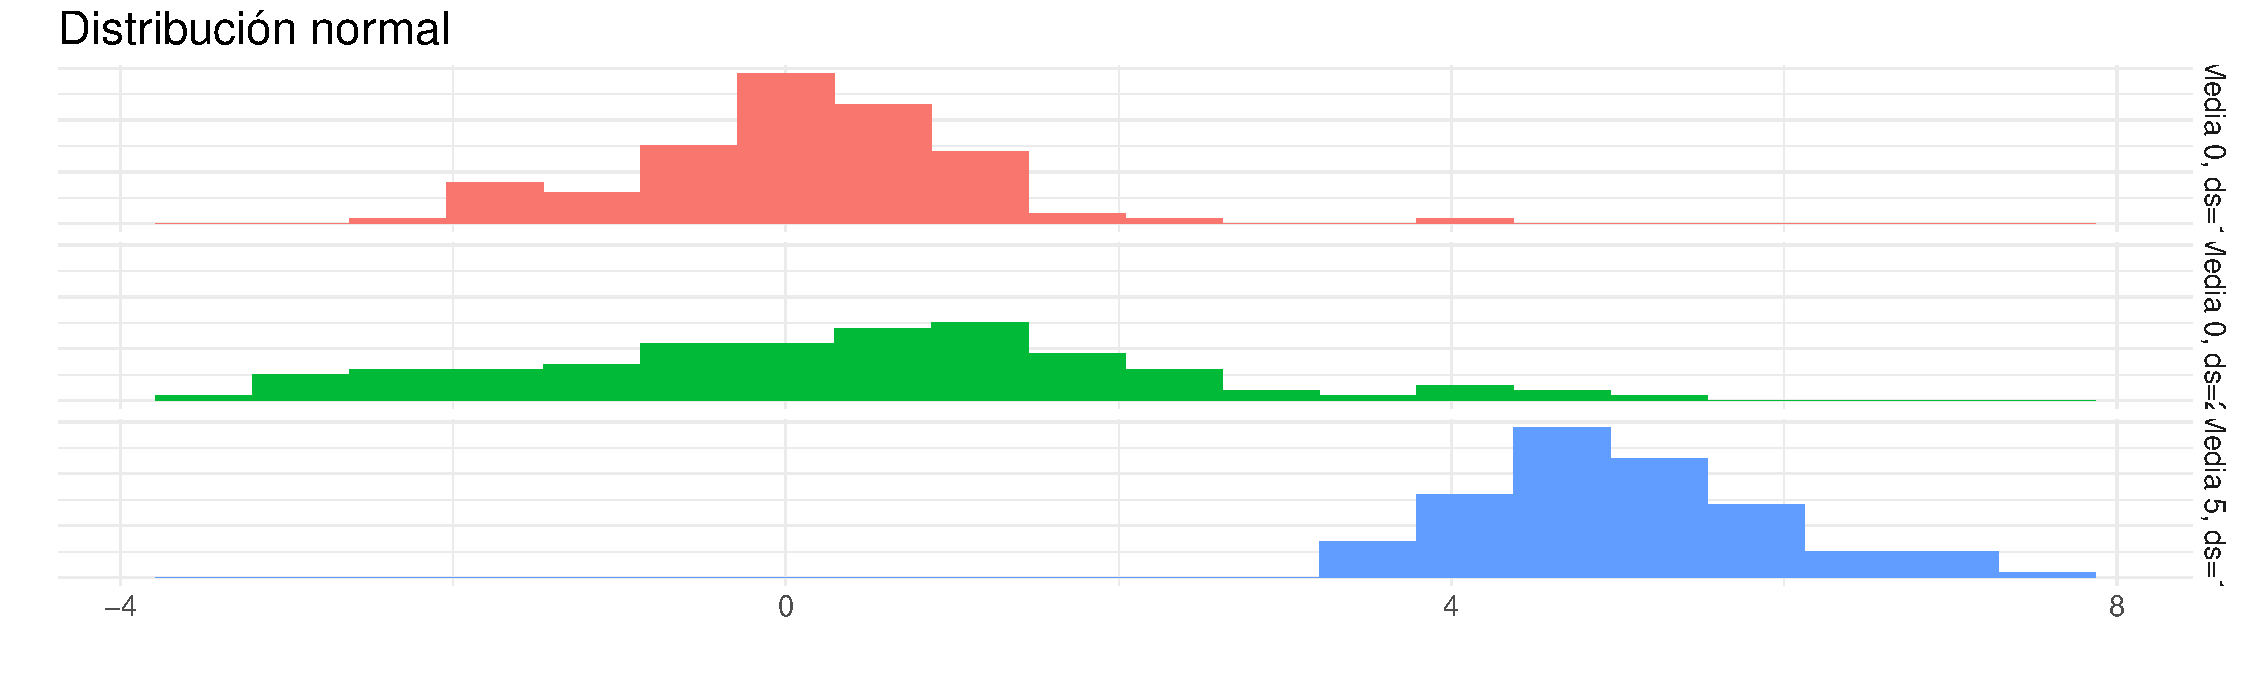
\includegraphics{bookdown_files/figure-latex/unnamed-chunk-41-2.pdf}

\hypertarget{kernel}{%
\subsubsection{Kernel}\label{kernel}}

Los Kernels son simplemente un suavizados sobre los histogramas

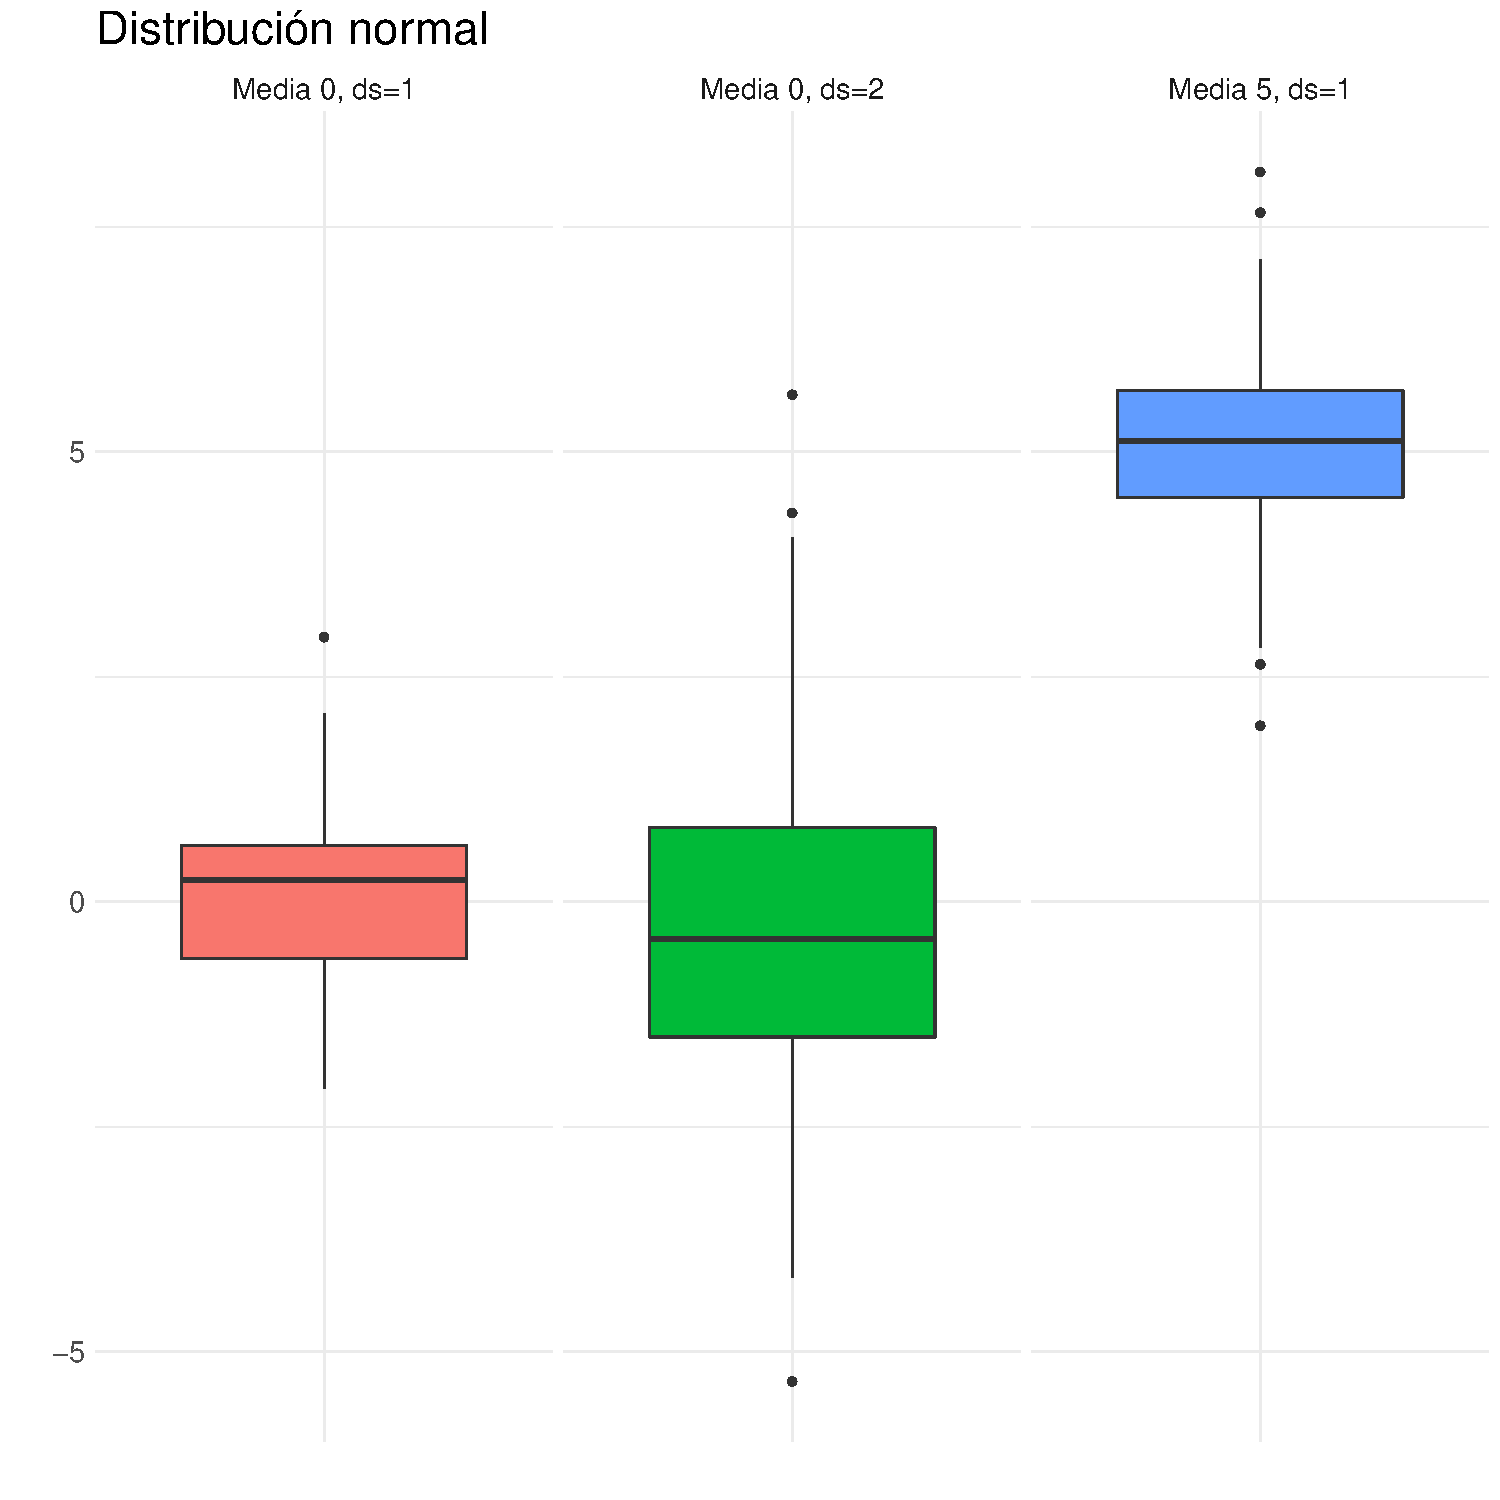
\includegraphics{bookdown_files/figure-latex/unnamed-chunk-42-1.pdf} 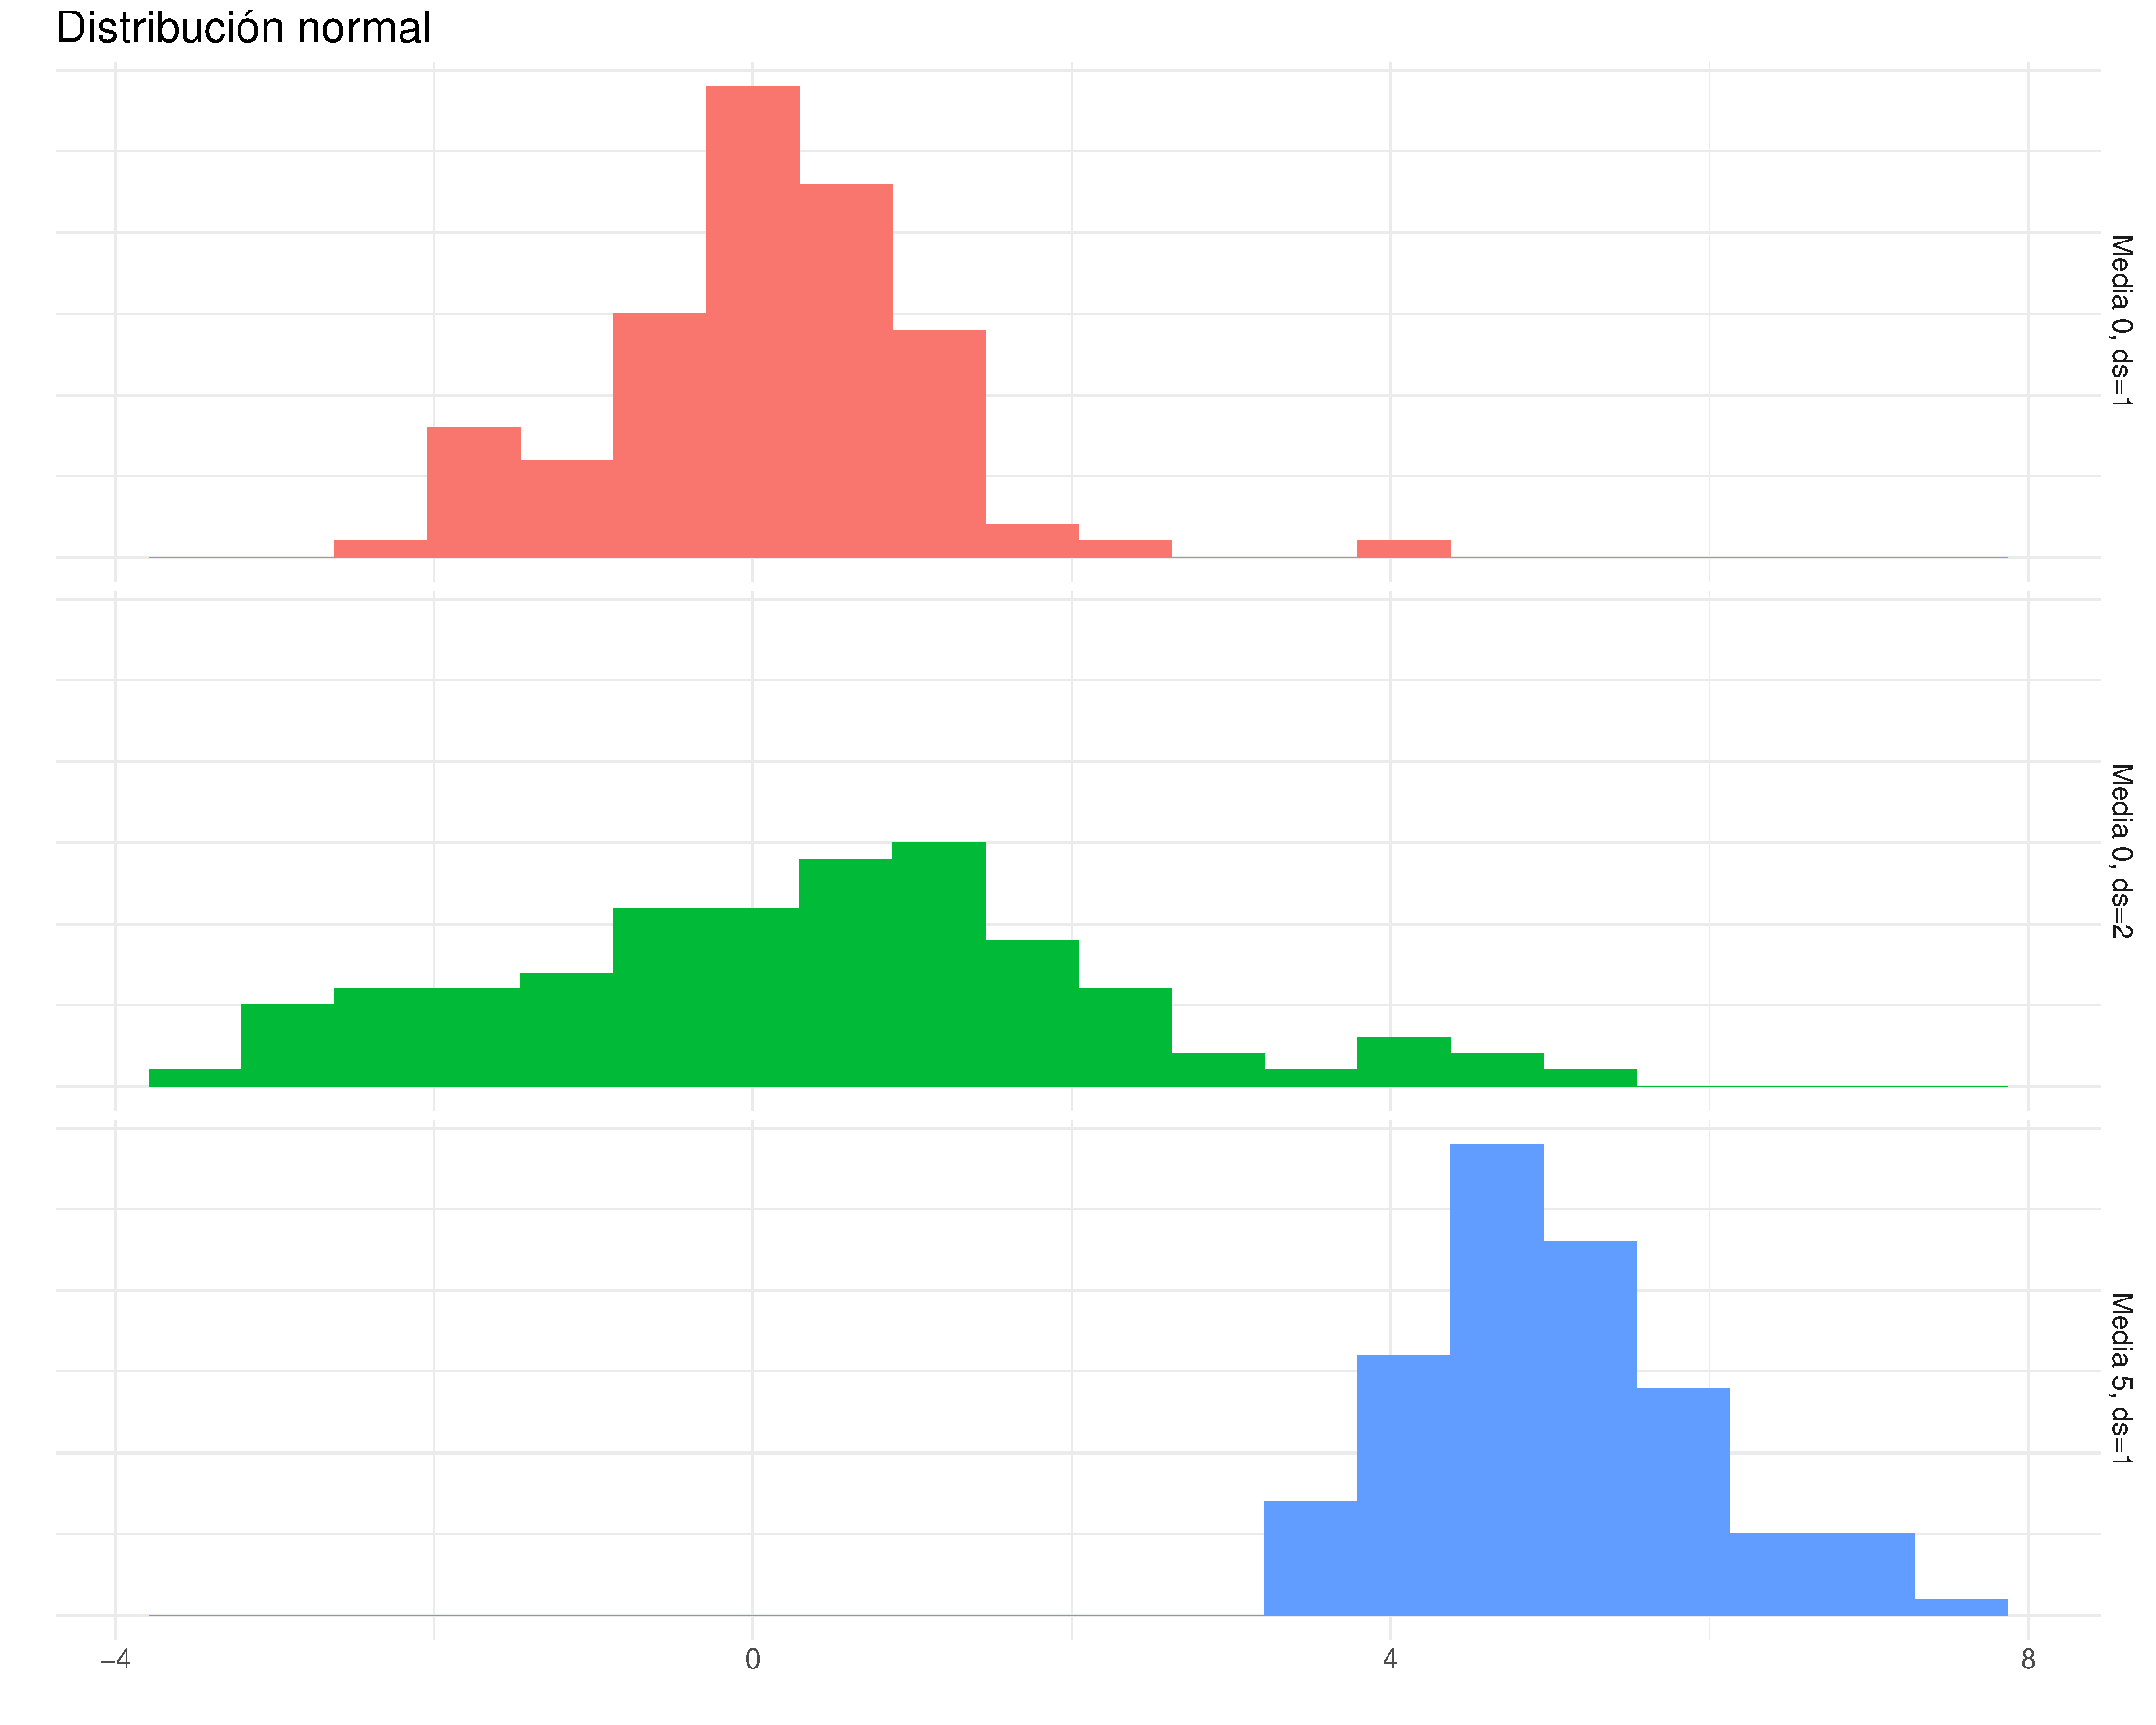
\includegraphics{bookdown_files/figure-latex/unnamed-chunk-42-2.pdf}

\hypertarget{violin-plots}{%
\subsubsection{Violin plots}\label{violin-plots}}

Combinando la idea de Kernels y boxplots, se crearon los violin plots, que simplemente muestran a los kernels duplicados

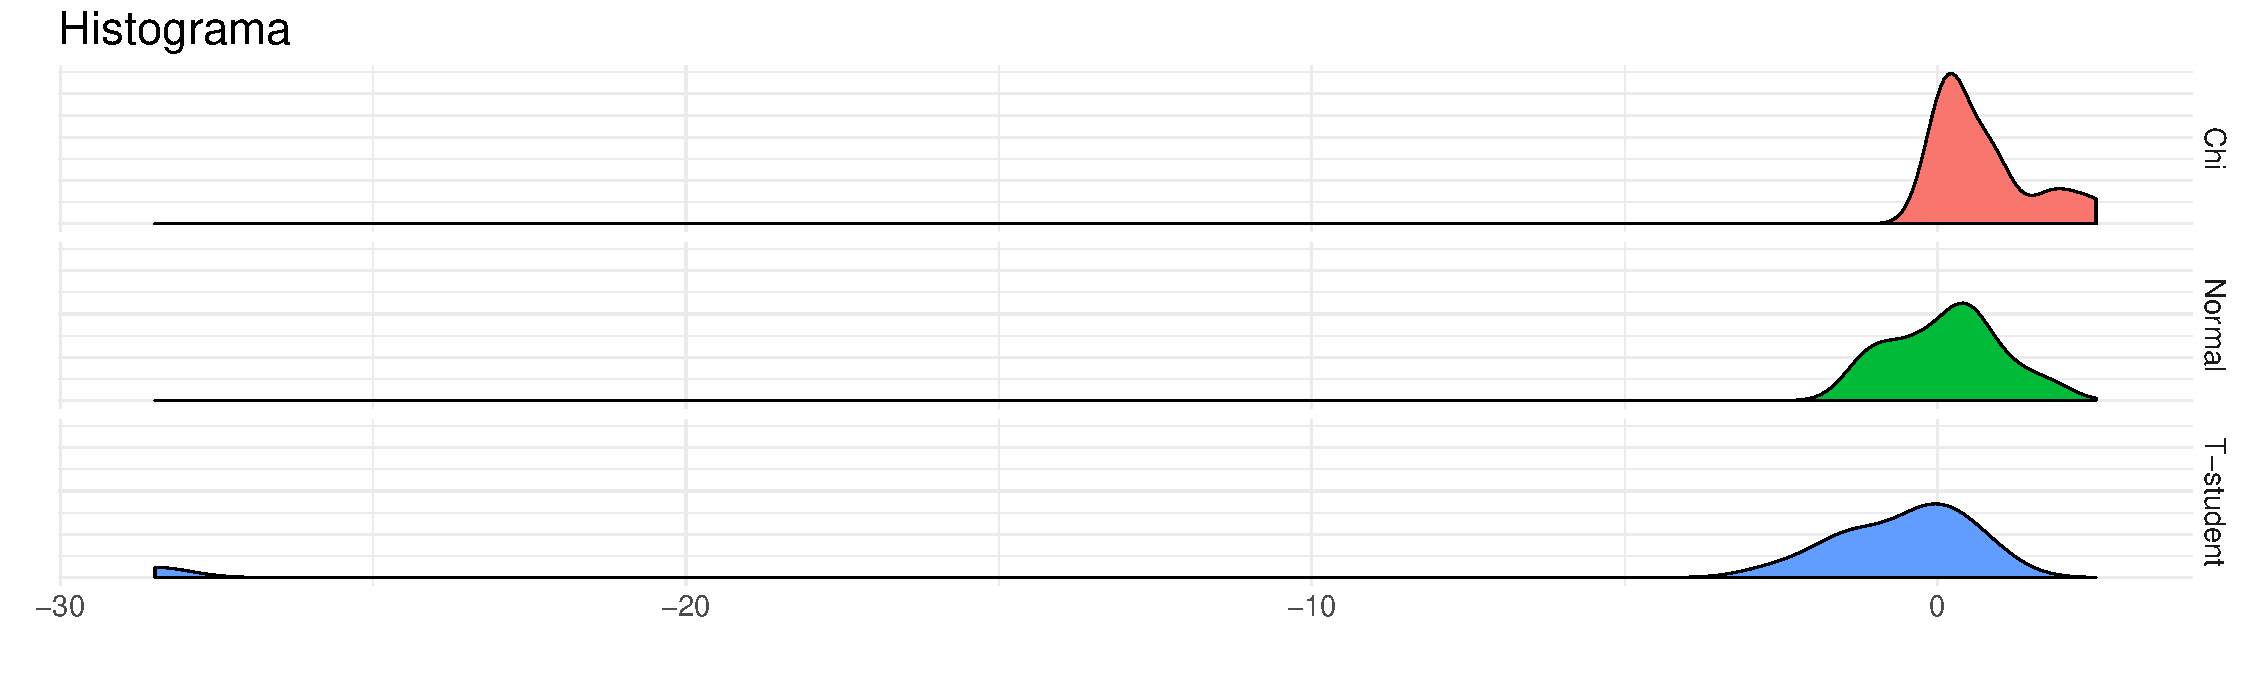
\includegraphics{bookdown_files/figure-latex/unnamed-chunk-43-1.pdf} 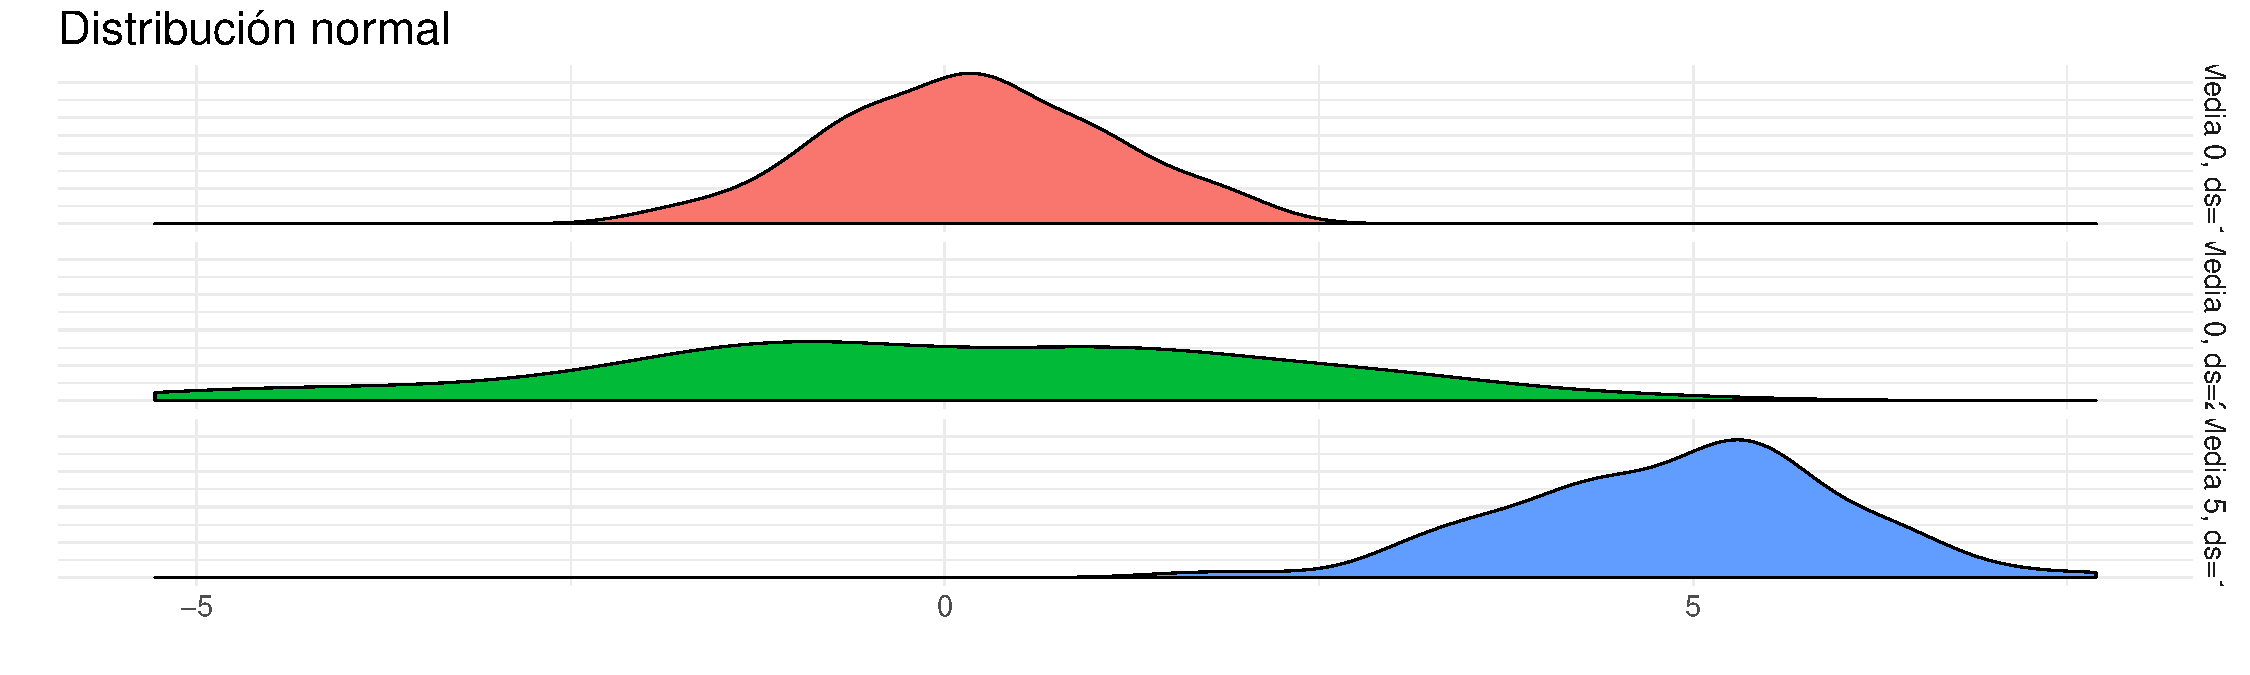
\includegraphics{bookdown_files/figure-latex/unnamed-chunk-43-2.pdf}

\hypertarget{practica-guiada-1}{%
\section{Práctica Guiada}\label{practica-guiada-1}}

\hypertarget{generacion-de-datos-aleatorios}{%
\subsection{Generación de datos aleatorios}\label{generacion-de-datos-aleatorios}}

Para generar datos aleatorios, usamos las funciones

-\texttt{rnorm} para generar datos que surgen de una distribución normal
-\texttt{rt} para generar datos que surgen de una distribución T-student
-\texttt{rchisq} para generar datos que surgen de una distribución Chi cuadrado

\begin{quote}
pero antes, tenemos que fijar la \emph{semilla} para que los datos sean reproducibles
\end{quote}

\begin{verbatim}
##  [1] -1.20706575  0.27742924  1.08444118 -2.34569770  0.42912469
##  [6]  0.50605589 -0.57473996 -0.54663186 -0.56445200 -0.89003783
## [11] -0.47719270 -0.99838644 -0.77625389  0.06445882  0.95949406
\end{verbatim}

\begin{verbatim}
##  [1] -0.363717710 -1.603466805 -0.388596796 -0.588007490  0.007839245
##  [6] 14.690527710 -1.863488555  0.022667470 -2.084247299 -0.249237745
## [11] -1.311594174 -3.569055208 -2.490838240 -3.848779244 -4.271087169
\end{verbatim}

\begin{verbatim}
##  [1] 0.5317744 1.4263809 4.2797098 0.2184660 0.6923773 0.0455256 3.1902100
##  [8] 0.2949942 0.5403827 0.1543732 0.8639196 0.1417290 1.1386091 0.2966193
## [15] 0.5110879
\end{verbatim}

Para poder ver rápidamente de qué se tratan los valores, podemos usar el comando plot
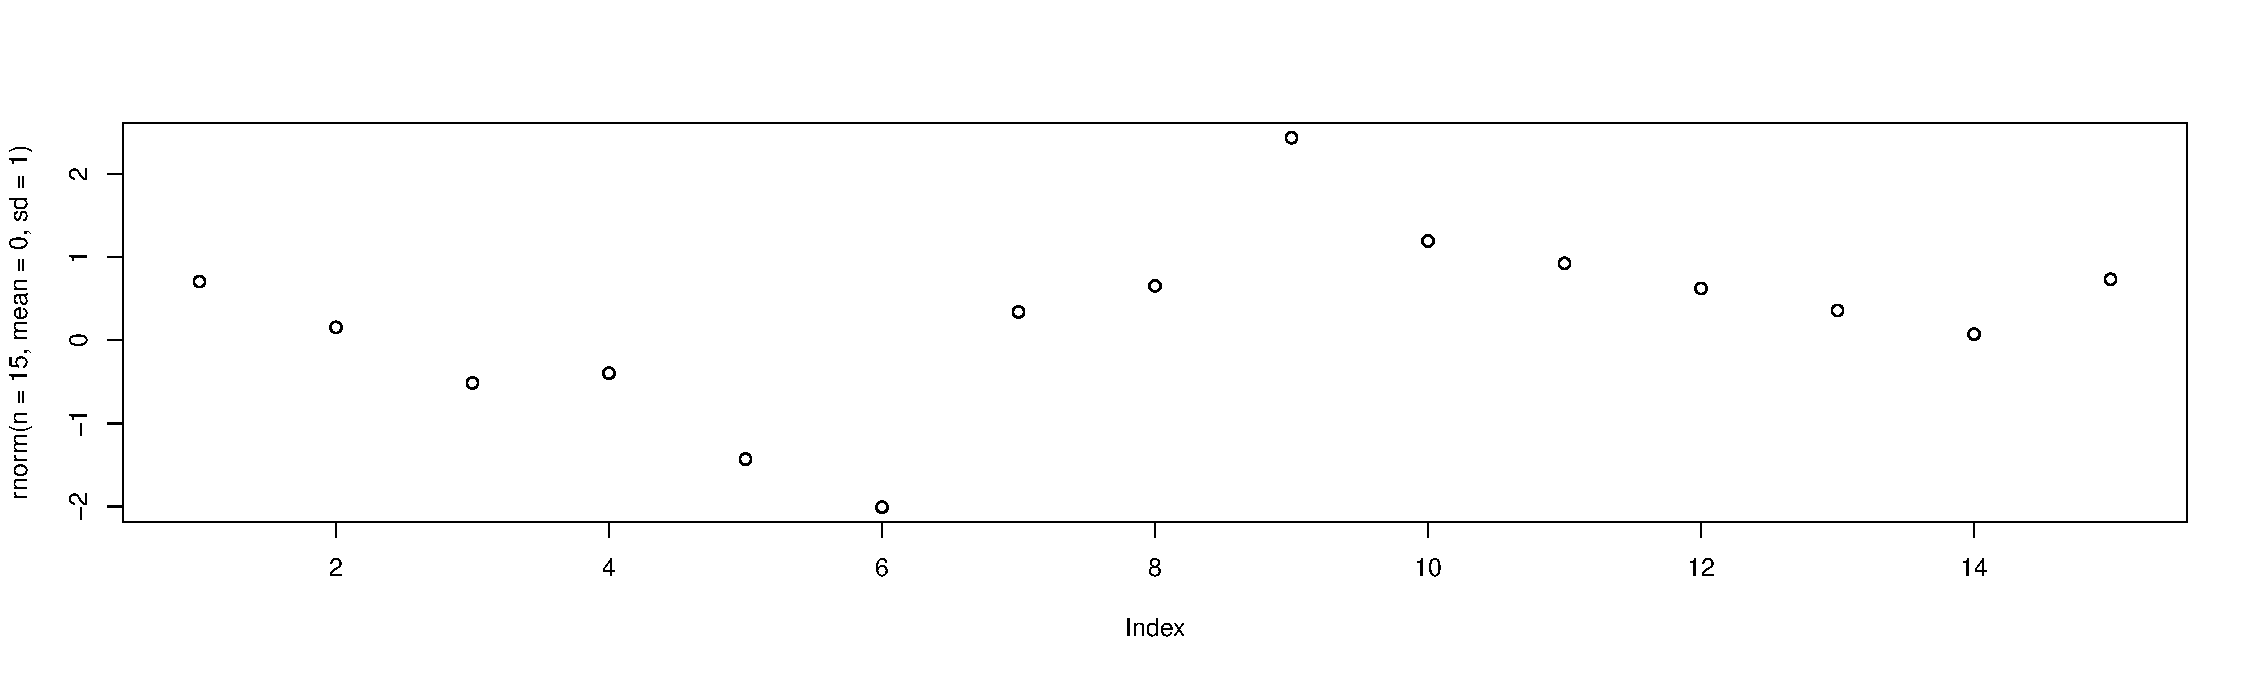
\includegraphics{bookdown_files/figure-latex/unnamed-chunk-46-1.pdf} 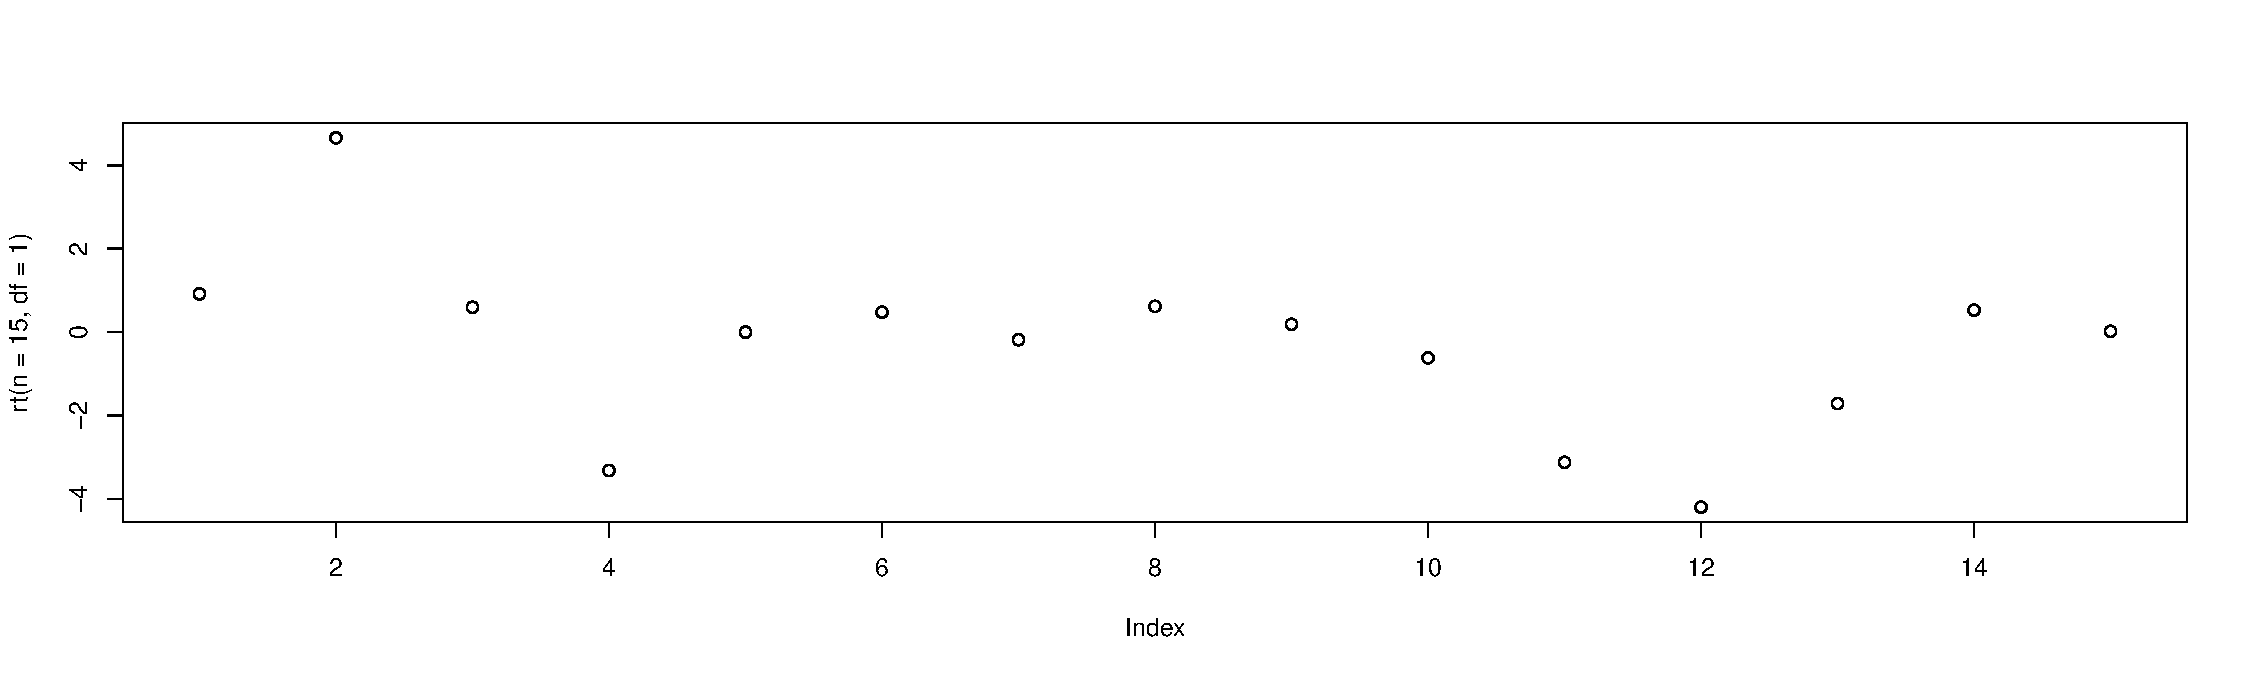
\includegraphics{bookdown_files/figure-latex/unnamed-chunk-46-2.pdf} 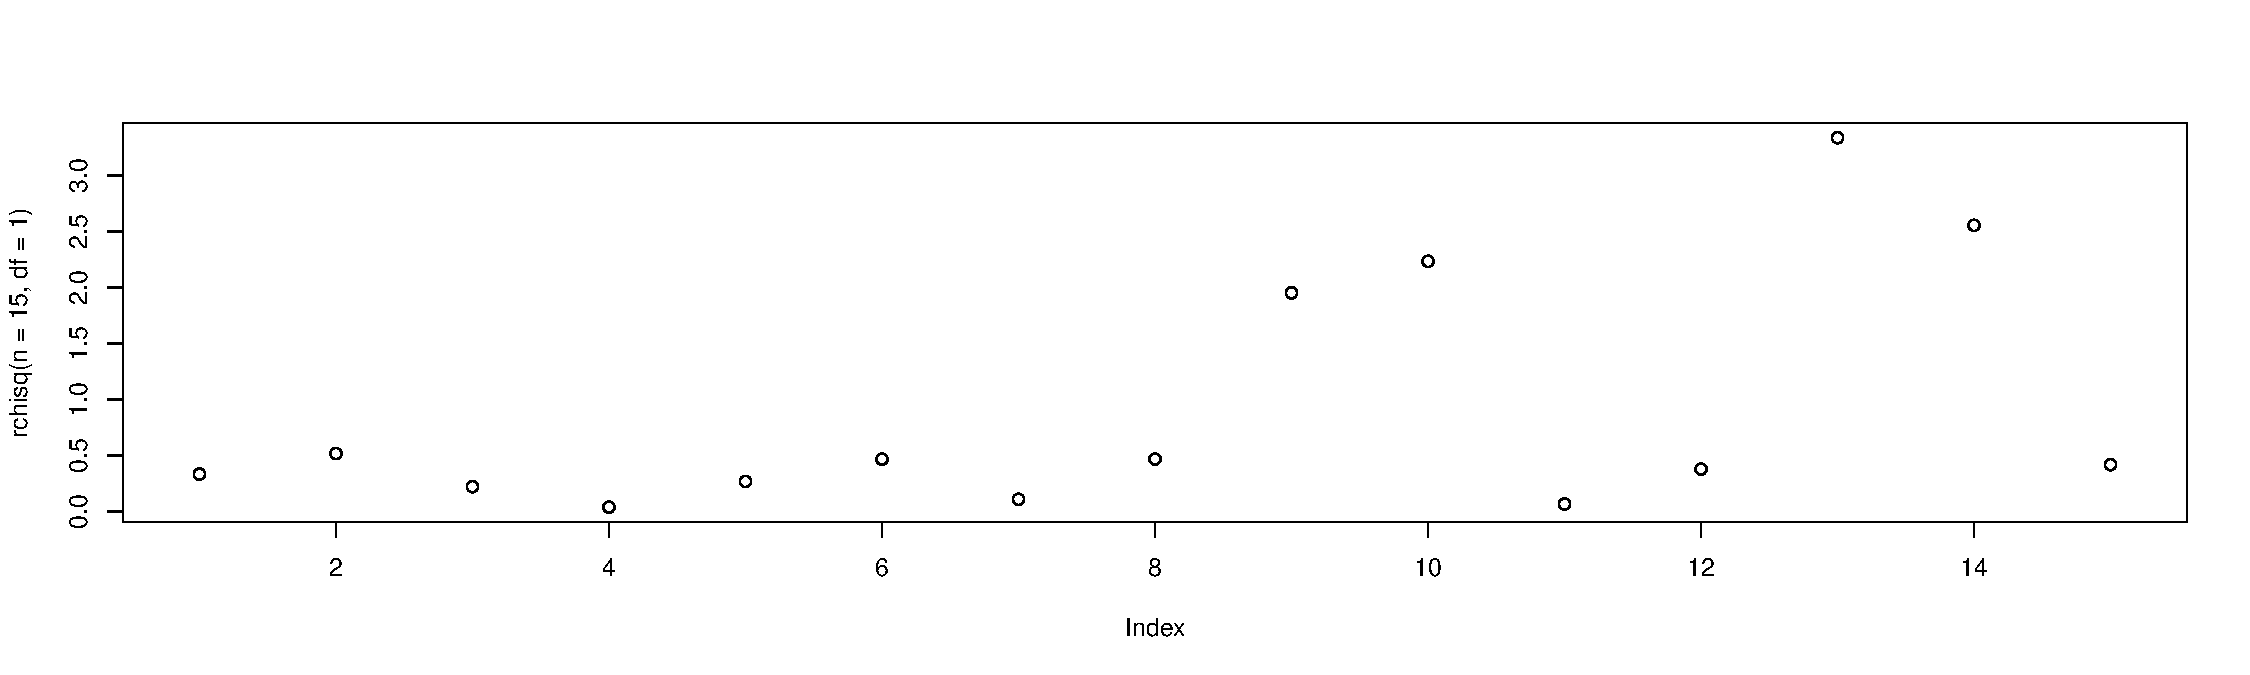
\includegraphics{bookdown_files/figure-latex/unnamed-chunk-46-3.pdf}

Noten que el eje X es el índice de los valores, es decir que no agrega información.

\hypertarget{tests}{%
\subsection{Tests}\label{tests}}

Utilicemos ahora datos reales.

los datos salen de \url{https://data.buenosaires.gob.ar/dataset/femicidios}

\begin{quote}
Vamos a ver ahora las estadisticas de Buenos Aires sobre la cantidad de femicidios por grupo etario. Es interesante preguntarse si hay más femicidios para cierto rango etario.
\end{quote}

\begin{verbatim}
## # A tibble: 19 x 3
##     anio cantidad_femicidios grupo_edad
##    <dbl> <chr>               <chr>     
##  1  2015 1                   0 - 15    
##  2  2015 2                   16 - 20   
##  3  2015 5                   21 - 40   
##  4  2015 3                   41 - 60   
##  5  2015 -                   61 y más  
##  6  2015 1                   Ignorado  
##  7  2016 2                   0 - 15    
##  8  2016 3                   16 - 20   
##  9  2016 4                   21 - 40   
## 10  2016 1                   41 - 60   
## 11  2016 2                   61 y más  
## 12  2016 2                   Ignorado  
## 13  2017 …                   0 - 15    
## 14  2017 …                   16 - 20   
## 15  2017 …                   21 - 40   
## 16  2017 …                   41 - 60   
## 17  2017 …                   61 y más  
## 18  2017 …                   Ignorado  
## 19  2017 9                   TOTAL
\end{verbatim}

fijense que las estadísitcas no estan desagregadas por rango etario para 2017, que en caso de que haya 0 femicidios pusieron `-' en lugar de 0. Además, como tenemos pocos datos, es mejor hacer un test que compare sólamente dos grupos.

Vamos a reorganizar la información para corregir todas estas cosas

\begin{verbatim}
## # A tibble: 2 x 2
##   grupo_edad cantidad_femicidios
##   <chr>                    <dbl>
## 1 0-40                        17
## 2 41 y más                     6
\end{verbatim}

Con esta tabla de contingencia podemos hacer un test de hipótesis.

¿Cuál usamos? Nos fijamos en el machete, o googleamos, y vemos que como queremos comparar la cantidad de casos por grupos categóricos, tenemos que usar el test Chi.

\begin{itemize}
\tightlist
\item
  \(H_0\) No hay asociación entre las variables
\item
  \(H_1\) Hay asociación entre las variables
\end{itemize}

La idea es que tenemos dos variables: El rango etario y la cantidad de femicidios

\begin{verbatim}
## 
##  Chi-squared test for given probabilities
## 
## data:  femicidios$cantidad_femicidios
## X-squared = 5.2609, df = 1, p-value = 0.02181
\end{verbatim}

noten que el resultado lo dan en términos del p-valor. Como el valor es bajo, menor a 0.05, entonces podemos rechazar que no existe relación. O en otros términos, pareciera que la diferencia es significativa estadísticamente.

\hypertarget{descripcion-estadistica-de-los-datos}{%
\subsection{Descripción estadística de los datos}\label{descripcion-estadistica-de-los-datos}}

Volveremos a ver los datos de \href{https://data.buenosaires.gob.ar/dataset/sueldo-funcionarios}{sueldos de funcionarios}

Con el comando \texttt{summary} podemos ver algunos de los principales estadísticos de resumen

\begin{verbatim}
##    Min. 1st Qu.  Median    Mean 3rd Qu.    Max. 
##  197746  210061  226866  225401  231168  249662
\end{verbatim}

\hypertarget{graficos-estadisticos-1}{%
\subsection{Gráficos estadísticos}\label{graficos-estadisticos-1}}

No nos vamos a detener demasiado a ver cómo hacer los gráficos de resumen, porque la próxima clase veremos como realizar gráficos de mejor calidad. Como los presentados en las notas de clase

A modo de ejemplo, dejamos los comandos de R base para realizar gráficos

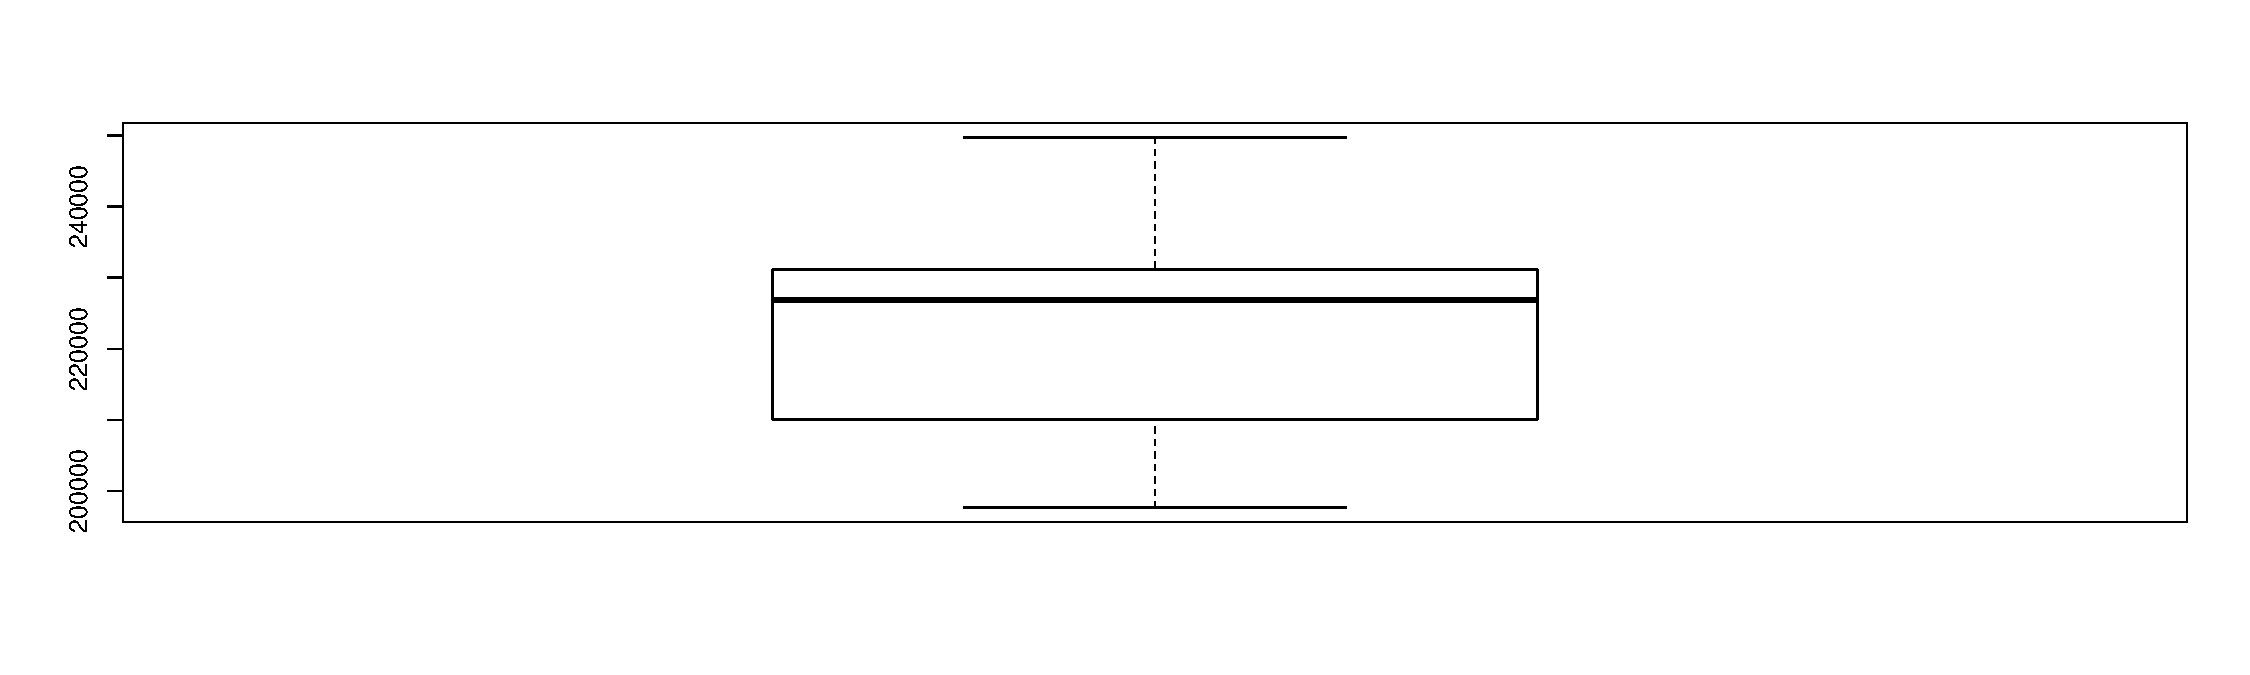
\includegraphics{bookdown_files/figure-latex/unnamed-chunk-52-1.pdf} 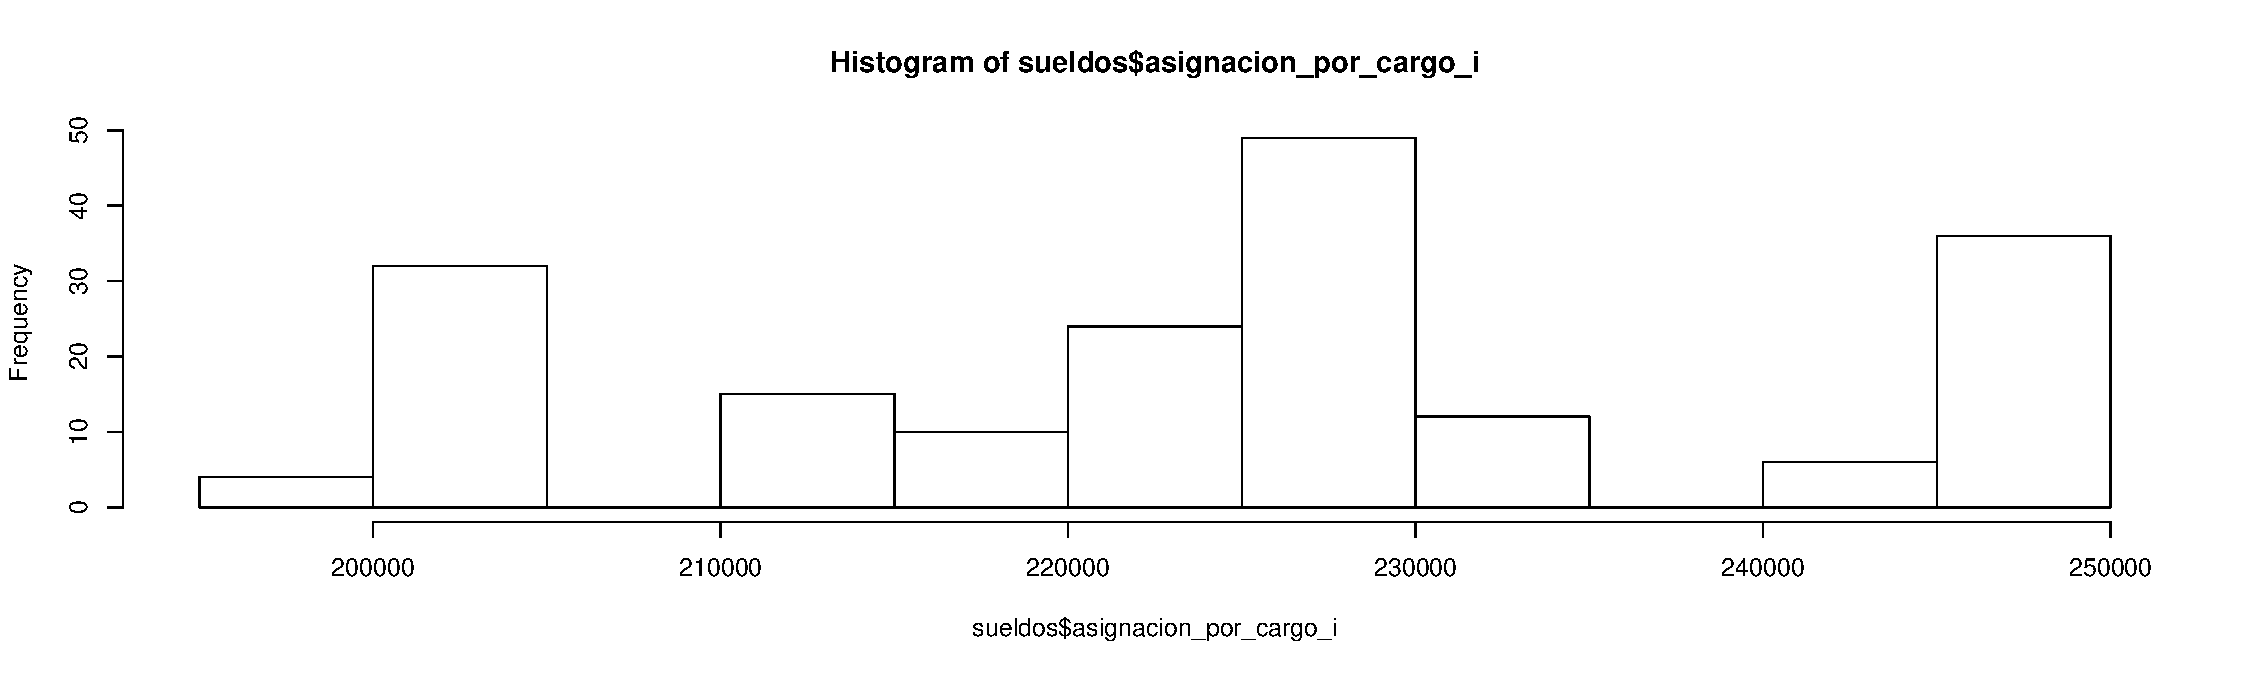
\includegraphics{bookdown_files/figure-latex/unnamed-chunk-52-2.pdf} 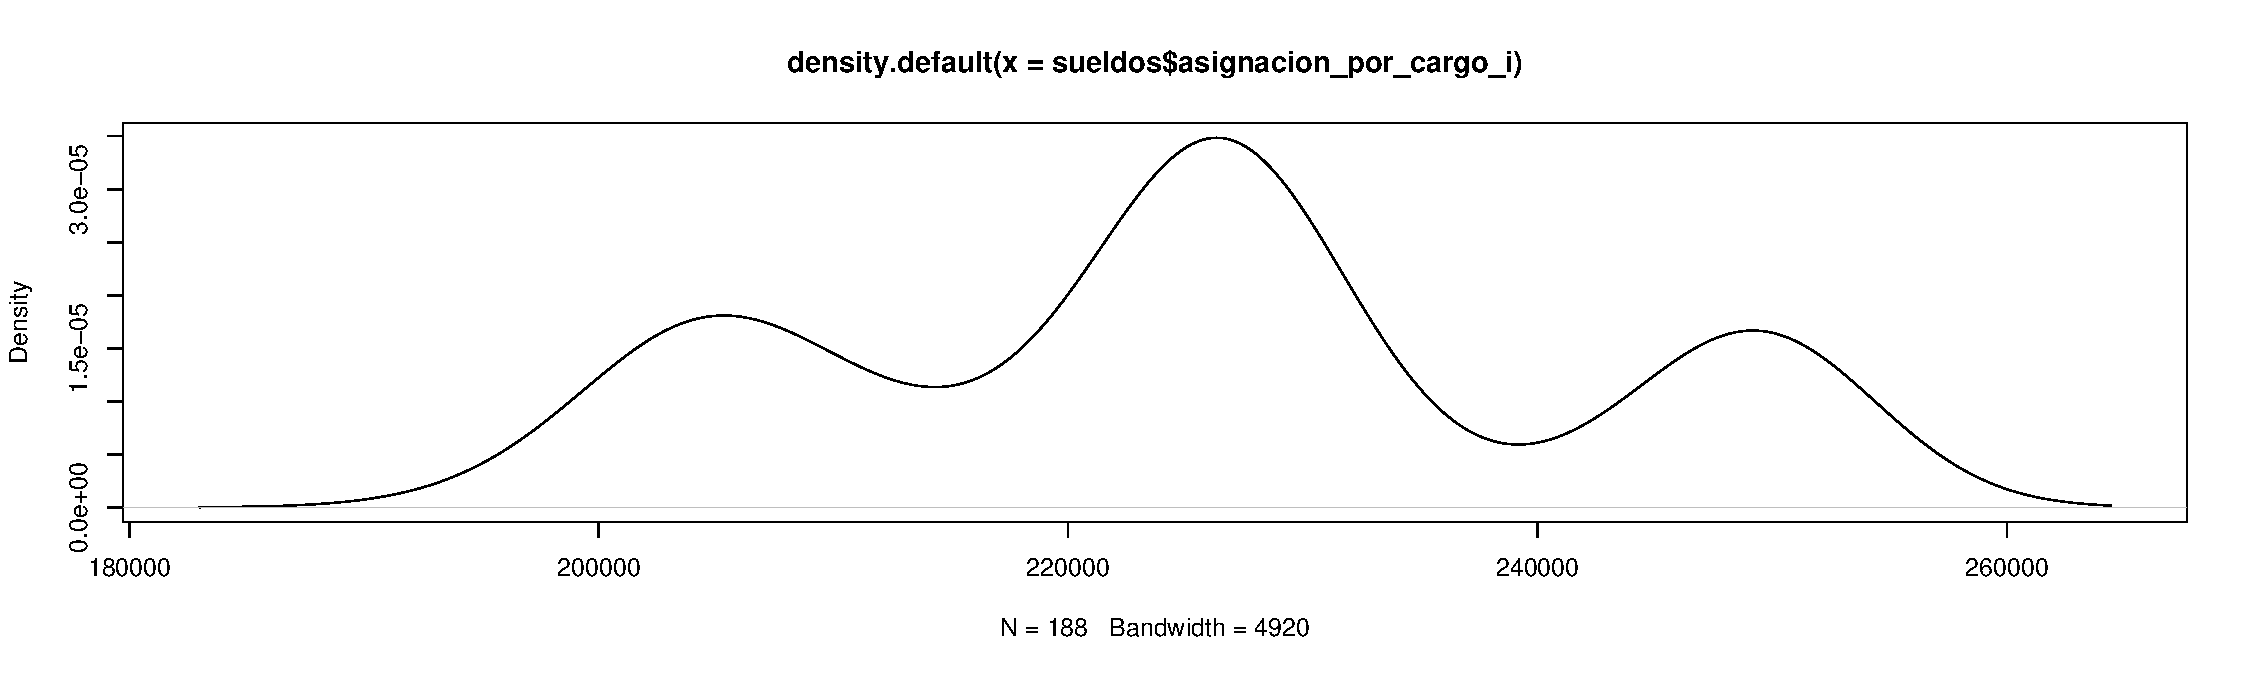
\includegraphics{bookdown_files/figure-latex/unnamed-chunk-52-3.pdf}

\bibliography{book.bib,packages.bib}


\end{document}
